\documentclass[aspectratio=169]{beamer}
% \mode<presentation>
\setbeamertemplate{navigation symbols}{}
\let\tempone\itemize
\let\temptwo\enditemize
\renewenvironment{itemize}{\tempone\addtolength{\itemsep}{0.5\baselineskip}}{\temptwo}

%%%%%%%%%%%%%%%%%%%%%%
\usepackage{beamerthemeshadow}
\usepackage[normalem]{ulem}
\usepackage{xcolor}
\usepackage{hyperref}
\usepackage{pgffor}
\usepackage{booktabs}
\usepackage{graphicx}
\usepackage{amssymb}
\usepackage{bbm}
\usepackage{tabularx}
\usepackage{tikz,etoolbox}
\usepackage{tikz,amsmath,siunitx}
\usetikzlibrary{arrows,snakes,backgrounds,patterns,matrix,shapes,fit,calc,shadows,plotmarks}
\usepackage{subcaption}
\usepackage{pgf}
\usepackage{latexsym}
\usepackage{amsfonts}
\usepackage{amssymb}
\usepackage{amsthm}
\usepackage[noend]{algpseudocode}
\usepackage{algorithm}
\usepackage{amsmath}
\usepackage{tabularx}
\usepackage{xcolor}
\usepackage[absolute,overlay]{textpos}
\usetikzlibrary{shapes,arrows,positioning,automata,positioning,spy,matrix,scopes,chains}
\newcommand{\digs}[2]{\hphantom{999}\llap{#1}\,+\,\hphantom{999}\llap{#2}}
\setbeamersize{text margin left=6mm}
\setbeamersize{text margin right=6mm}
\renewcommand{\insertnavigation}[1]{}
\setbeamertemplate{headline}{}
\setbeamertemplate{footline}{}
\usefonttheme{professionalfonts}
\setbeamercovered{transparent}
\mode<presentation>
\linespread{1.25}
\newcommand{\thetitle}[1]{{\begin{center}\structure{{#1}}\end{center}}}
\DeclareMathOperator{\Tr}{Tr} 
\DeclareMathOperator{\JSD}{JSD} 

\newcommand{\boldA}{\boldsymbol{A}}
\newcommand{\boldB}{\boldsymbol{B}}
\newcommand{\boldC}{\boldsymbol{C}}
\newcommand{\boldD}{\boldsymbol{D}}
\newcommand{\boldE}{\boldsymbol{E}}
\newcommand{\boldF}{\boldsymbol{F}}
\newcommand{\boldG}{\boldsymbol{G}}
\newcommand{\boldH}{\boldsymbol{H}}
\newcommand{\boldI}{\boldsymbol{I}}
\newcommand{\boldJ}{\boldsymbol{J}}
\newcommand{\boldK}{\boldsymbol{K}}
\newcommand{\boldL}{\boldsymbol{L}}
\newcommand{\boldM}{\boldsymbol{M}}
\newcommand{\boldN}{\boldsymbol{N}}
\newcommand{\boldO}{\boldsymbol{O}}
\newcommand{\boldP}{\boldsymbol{P}}
\newcommand{\boldQ}{\boldsymbol{Q}}
\newcommand{\boldR}{\boldsymbol{R}}
\newcommand{\boldS}{\boldsymbol{S}}
\newcommand{\boldT}{\boldsymbol{T}}
\newcommand{\boldU}{\boldsymbol{U}}
\newcommand{\boldV}{\boldsymbol{V}}
\newcommand{\boldW}{\boldsymbol{W}}
\newcommand{\boldX}{\boldsymbol{X}}
\newcommand{\boldY}{\boldsymbol{Y}}
\newcommand{\boldZ}{\boldsymbol{Z}}
\newcommand{\bolda}{\boldsymbol{a}}
\newcommand{\boldb}{\boldsymbol{b}}
\newcommand{\boldc}{\mathbf{c}}
\newcommand{\boldd}{\boldsymbol{d}}
\newcommand{\bolde}{\boldsymbol{e}}
\newcommand{\boldf}{\boldsymbol{f}}
\newcommand{\boldg}{\boldsymbol{g}}
\newcommand{\boldh}{\boldsymbol{h}}
\newcommand{\boldi}{\boldsymbol{i}}
\newcommand{\boldj}{\boldsymbol{j}}
\newcommand{\boldk}{\boldsymbol{k}}
\newcommand{\boldl}{\boldsymbol{l}}
\newcommand{\boldm}{\boldsymbol{m}}
\newcommand{\boldn}{\boldsymbol{n}}
\newcommand{\boldo}{\boldsymbol{o}}
\newcommand{\boldp}{\boldsymbol{p}}
\newcommand{\boldq}{\boldsymbol{q}}
\newcommand{\boldr}{\boldsymbol{r}}
\newcommand{\bolds}{\boldsymbol{s}}
\newcommand{\boldt}{\boldsymbol{t}}
\newcommand{\boldu}{\boldsymbol{u}}
\newcommand{\boldv}{\boldsymbol{v}}
\newcommand{\boldw}{\boldsymbol{w}}
\newcommand{\boldx}{\mathbf{x}}
\newcommand{\boldy}{\boldsymbol{y}}
\newcommand{\boldz}{\mathbf{z}}

\newcommand{\mcA}{\mathcal{A}}
\newcommand{\mcB}{\mathcal{B}}
\newcommand{\mcC}{\mathcal{C}}
\newcommand{\mcD}{\mathcal{D}}
\newcommand{\mcE}{\mathcal{E}}
\newcommand{\mcF}{\mathcal{F}}
\newcommand{\mcG}{\mathcal{G}}
\newcommand{\mcH}{\mathcal{H}}
\newcommand{\mcI}{\mathcal{I}}
\newcommand{\mcJ}{\mathcal{J}}
\newcommand{\mcK}{\mathcal{K}}
\newcommand{\mcL}{\mathcal{L}}
\newcommand{\mcM}{\mathcal{M}}
\newcommand{\mcN}{\mathcal{N}}
\newcommand{\mcO}{\mathcal{O}}
\newcommand{\mcP}{\mathcal{P}}
\newcommand{\mcQ}{\mathcal{Q}}
\newcommand{\mcR}{\mathcal{R}}
\newcommand{\mcS}{\mathcal{S}}
\newcommand{\mcT}{\mathcal{T}}
\newcommand{\mcU}{\mathcal{U}}
\newcommand{\mcV}{\mathcal{V}}
\newcommand{\mcW}{\mathcal{W}}
\newcommand{\mcX}{\mathcal{X}}
\newcommand{\mcY}{\mathcal{Y}}
\newcommand{\mcZ}{\mathcal{Z}}

\newcommand{\reals}{\ensuremath{\mathbb{R}}}
\newcommand{\integers}{\ensuremath{\mathbb{Z}}}
\newcommand{\rationals}{\ensuremath{\mathbb{Q}}}
\newcommand{\naturals}{\ensuremath{\mathbb{N}}}
\newcommand{\trans}{\ensuremath{\mathsf{T}}}
\newcommand{\ident}{\boldsymbol{I}}
\newcommand{\bzero}{\boldsymbol{0}}

\newcommand{\balpha}{\boldsymbol{\alpha}}
\newcommand{\bbeta}{\boldsymbol{\beta}}
\newcommand{\bdelta}{\boldsymbol{\delta}}
\newcommand{\boldeta}{\boldsymbol{\eta}}
\newcommand{\bkappa}{\boldsymbol{\kappa}}
\newcommand{\bgamma}{\boldsymbol{\gamma}}
\newcommand{\bmu}{\boldsymbol{\mu}}
\newcommand{\bphi}{\boldsymbol{\phi}}
\newcommand{\bpi}{\boldsymbol{\pi}}
\newcommand{\bpsi}{\boldsymbol{\psi}}
\newcommand{\bsigma}{\boldsymbol{\sigma}}
\newcommand{\btheta}{\boldsymbol{\theta}}
\newcommand{\bxi}{\boldsymbol{\xi}}
\newcommand{\bGamma}{\boldsymbol{\Gamma}}
\newcommand{\bLambda}{\boldsymbol{\Lambda}}
\newcommand{\bOmega}{\boldsymbol{\Omega}}
\newcommand{\bPhi}{\boldsymbol{\Phi}}
\newcommand{\bPi}{\boldsymbol{\Pi}}
\newcommand{\bPsi}{\boldsymbol{\Psi}}
\newcommand{\bSigma}{\boldsymbol{\Sigma}}
\newcommand{\bTheta}{\boldsymbol{\Theta}}
\newcommand{\bUpsilon}{\boldsymbol{\Upsilon}}
\newcommand{\bXi}{\boldsymbol{\Xi}}
\newcommand{\bepsilon}{\boldsymbol{\epsilon}}

\def\argmin{\operatornamewithlimits{arg\,min}}
\def\argmax{\operatornamewithlimits{arg\,max}}

\newcommand{\given}{\,|\,}
\newcommand{\param}{; \,}

\newcommand{\distNorm}{\mathcal{N}}

\newcommand{\E}{\mathbb{E}}
\newcommand{\ind}{\mathbb{1}}
\newcommand{\Hess}{\mathrm{H}}
\DeclareMathOperator*{\KL}{KL}
\DeclareMathOperator*{\ELBO}{ELBO}
\DeclareMathOperator*{\RELU}{ReLU}
\DeclareMathOperator*{\MLP}{MLP}
\DeclareMathOperator*{\LSTM}{LSTM}
\DeclareMathOperator*{\RNN}{RNN}
\DeclareMathOperator*{\RNNLM}{RNNLM}
\DeclareMathOperator*{\softmax}{softmax}
\DeclareMathOperator*{\enc}{enc}
\DeclareMathOperator*{\gen}{gen}
\DeclareMathOperator*{\sal}{sal}
\DeclareMathOperator*{\encsal}{input-sal}
\DeclareMathOperator*{\clip}{clip}


\usepackage{color}
\usepackage{multirow}
\usepackage{rotating}
\usepackage[all,dvips]{xy}
\usepackage{colortbl}
\usepackage{graphicx}
\usepackage{verbatim}
\usepackage{framed}
\usepackage{natbib}
\usepackage[labelformat=empty]{caption}
\newcommand{\air}{\vspace{0.25cm}}
\newcommand{\mair}{\vspace{-0.25cm}}

\setbeamertemplate{navigation symbols}{}%remove navigation symbols
\renewcommand{\rmdefault}{crm}
\definecolor{vermillion}{RGB}{213,94,0}
\definecolor{orange}{RGB}{230,159,0}
\definecolor{skyblue}{RGB}{86,180,233}
\definecolor{bluegreen}{RGB}{90,143,41}
% \definecolor{bluegreen}{RGB}{0,158,115}
\definecolor{myyellow}{RGB}{240,228,66} % i dunno if this is the same as standard yellow
\definecolor{myblue}{RGB}{0,114,178}
\definecolor{vermillion}{RGB}{213,94,0}
\definecolor{redpurple}{RGB}{204,121,167}
\definecolor{lightgrey}{RGB}{234,234,234}
\usepackage{tikz}
\usetikzlibrary{fit,positioning}
\usetikzlibrary{bayesnet}
\usetikzlibrary{arrows}
\usetikzlibrary{decorations.pathreplacing}
% \setbeamerfont{alerted text}{series=\bfseries}
% \setbeamerfont{structure}{series=\bfseries}
% Needed for diakgrams.
\def\im#1#2{
  \node(#1) [scale=#2]{\pgfbox[center,top]{\pgfuseimage{#1}}
};}
% \input{pictures_header}
% make smaller citations
\let\realcitep\citep
\renewcommand*{\citep}[1]{{\scriptsize \realcitep{#1}}}
\let\realcitet\citet
\renewcommand*{\citet}[1]{{\scriptsize \realcitet{#1}}}
\setcitestyle{square,semicolon,aysep={}} 

%%%%%%%%%%%%%%%%%%%%%%%%%%%%%%%%%%%%%%%%%%%%%%%%%%%%

\title[Tutorial: \\ Deep Latent NLP]{Deep Latent Variable Models  \\ of Natural Language}
\author[]{Yoon Kim, Sam Wiseman, Alexander Rush}
\institute[Harvard SEAS]{ 
  \begin{center}
    
\includegraphics[width=5cm]{harvardnlp}
  \end{center}
  \vspace{0.5cm}
  { \Large Tutorial 2018}
}
\date{}
%\usetheme{Madrid}
\usetheme[hideothersubsections]{Hannover}
\definecolor{darkgreen}{rgb}{0.13, 0.55, 0.13}
\definecolor{darkpurple}{rgb}{0.55, 0.0, 0.55}

\AtBeginSection[]
{
  \begin{frame}
  \tableofcontents[currentsection,hideothersubsections]
  \end{frame}
}

\AtBeginSubsection[]
{
  \begin{frame}
  \tableofcontents[currentsubsection]
  \end{frame}
}


\def\argmax{\operatornamewithlimits{arg\,max}}
\def\kargmax{\operatornamewithlimits{K-arg\,max}}
\setbeamercovered{transparent}


\begin{document}

\begin{frame}
  \titlepage
\end{frame}

\section{Introduction}

%
\subsection{Goals}

\begin{frame}{}
\thetitle{Goal of \underline{Latent-Variable} Modeling}
    Probabilistic models provide a declarative language for specifying 
    prior knowledge and structural relationships in the context of unknown variables.
    \vspace{0.5cm}
    \pause 
    
    Makes it easy to specify:
    \begin{itemize}
        \item Known interactions in the data
        \item Uncertainty about unknown factors
        \item Constraints on model properties
    \end{itemize}
\end{frame}

\begin{frame}{}
\thetitle{Latent-Variable Modeling in NLP}
    Long and rich history of latent-variable models of natural language. 
    \vspace{0.5cm}
        
    Major successes include, among many others:
    \begin{itemize}
        \item Statistical alignment for translation \cite{} 
        \item Document clustering and topic modeling \cite{}  
        \item Unsupervised part-of-speech tagging and parsing \cite{}
    \end{itemize}
    \air 
    
\end{frame}


\begin{frame}{}
\thetitle{Goals of \underline{Deep Learning}}
    Toolbox of methods for learning rich, non-linear 
    data representations through numerical optimization. 
    \vspace{0.5cm}
    
    \pause 
    Makes it easy to fit:
    \begin{itemize}
        \item Highly-flexible predictive models 
        \item Transferable feature representations 
        \item Structurally-aligned network architectures 
    \end{itemize}
    
\end{frame}

\begin{frame}
\thetitle{Deep Learning in NLP}
    Current dominant paradigm for NLP.
    \vspace{0.5cm}

    Major successes include, among many others:
    \begin{itemize}
        \item Text classification  \cite{}  
        \item Neural machine translation \cite{} 
        \item NLU Tasks (QA, NLI, etc) \cite{}
    \end{itemize}
\end{frame}

\begin{frame}{}
\thetitle{Tutorial: Deep Latent-Variable Models for NLP}
    \begin{itemize}
        \item 

    How should a contemporary ML/NLP researcher reason about latent-variables?
    \vspace{0.5cm}

        \item 
   
    What unique challenges come from modeling text with latent variables?   

    \vspace{0.5cm}

        \item 
   
    What techniques have been explored and shown to be effective in recent papers? 
    \end{itemize}
 

   
    %Two complementary and intersecting ideas:
    %\begin{enumerate}
    %    \item Inference in deep latent-variable models
    %    \air 
    %    \item Deep learning-based inference for latent variable models
    %\end{enumerate}
    %\vspace{0.5cm}
    \pause
    \air
    
    We explore these through the lens of \textit{variational inference}.    
    %This tutorial focuses on variational inference in both settings.
\end{frame}


\begin{frame}{}
\thetitle{Tutorial Take-Aways}



 \begin{enumerate}
    \item A collection of deep latent-variable \structure{models} for NLP
    \air
    
    \item An understanding of a \structure{variational} objective
    \air
    
    \item A toolkit of algorithms for \structure{optimization}
    
    \air
    \item A formal guide to \structure{advanced} techniques
    \air 
        
    \item A survey of example \structure{applications}
    \air
    
    \item Code samples and techniques for \structure{practical} use
 \end{enumerate}
    
\end{frame}

\begin{frame}{}
\thetitle{Tutorial Non-Objectives}
    Not covered (for time, not relevance):
    \begin{itemize}
        \item Many classical latent-variable approaches.
            \air
           
            
        \item Undirected graphical models such as MRFs
            \air
        
            
        \item Non-likelihood based models such as GANs
            \air
        
        \item Sampling-based inference such as MCMC.
            \air 

        \item Details of deep learning architectures.
    \end{itemize}
\end{frame}


\subsection{Background}

\begin{frame}
\thetitle{What are deep networks?}
Deep networks are parameterized non-linear functions; They transform input $\boldz$ into features $\boldh$ 
using parameters $\pi$. 


\vspace{0.5cm}
Important examples: The multilayer perceptron,
\begin{align*}
\boldh = \MLP(\boldz \param \pi) = \boldV \sigma (\boldW  \boldz + \boldb) + \bolda \ \ \ \ \  \pi = \{ \boldV, \boldW,  \bolda, \boldb\},
\end{align*}

\pause 
The recurrent neural network, which maps a sequence of inputs $\boldz_{1:T}$ into a sequence of features $\boldh_{1:T}$,
\begin{align*}
\boldh_{t} =  \RNN(\boldh_{t-1}, \boldz_t \param \pi) = \sigma (\boldU  \boldz_t + \boldV \boldh_{t-1} + \boldb) \ \ \ \ \  \pi = \{ \boldV, \boldU, \boldb\}
%\theta = \{ \boldW, \boldV, \boldU, \boldb\}$
%\softmax (\boldW \boldh_t),
\end{align*}.

% \begin{align*}
% \boldh_t = \RNN(\boldz_t, \boldh_{t-1} \param \theta) = \sigma (\boldW  \boldz_t + \boldV \boldh_{t-1} + \boldb) \ \ \\  \theta = \{ \boldV, \boldW, \boldb\}.
% \end{align*}
\end{frame}


\begin{frame}
\thetitle{What are latent variable models?}

Latent variable models give us a joint distribution
\begin{align*}
p(x, z \param \theta).
\end{align*}

\pause
\begin{itemize}
    \item $x$ is our observed data
    \item $z$ is a collection of latent variables
    \item $\theta$ are the deterministic parameters of the model, such as the neural network parameters
\end{itemize}

\pause

\begin{itemize}
    \item Data consists of $N$ i.i.d samples,
\end{itemize}


                \[ p(x^{(1:N)}, z^{(1:N)} \param \theta ) = \prod_{n=1}^N p(x^{(n)} \given z^{(n)}; \theta) p(z^{(n)};\theta). \]

\end{frame}

\begin{frame}
    \thetitle{Probabilistic Graphical Models}
    
    \begin{itemize}
        %\item $\Delta^{K-1}$ is the simplex over $K$ items, informally the space of distributions of $K$ discrete choices
        %\item $\softmax: \reals^t \mapsto \Delta^{k-1}$ is the mapping to the simplex defined by $\softmax(\boldh)_k \propto \exp(\boldh_k)$
        \item A directed PGM shows the conditional independence structure. 
        \item  By chain rule, latent variable model over observations can be represented as, 
        \begin{figure}
        \centering
        \begin{tikzpicture}
          %\tikz{
        % nodes
         \node[obs] (x1) {$x^{(n)}$};%
         \node[latent, above = of x1] (z) {$z^{(n)}$}; %
         %\node[const, above=of z] (mu) {$\bmu$};
         \node[const, left = of z] (pi) {$\theta$};
         \plate {plate1} {(x1)(z)} {$N$}; %
         \edge {z} {x1};
         \edge {pi.east} {x1};
         \edge {pi.east} {z};

         %}
         
         \end{tikzpicture}
                \[ p(x^{(1:N)}, z^{(1:N)} \param \theta) = \prod_{n=1}^N p(x^{(n)} \given z^{(n)}; \theta) p(z^{(n)};\theta) \]
 
         \end{figure}
                 \item Specific models may factor further.

    \end{itemize}
        

\end{frame}

\begin{frame}\thetitle{Posterior Inference}
    For all 
\end{frame}

\begin{frame}
    \thetitle{Problem Statement: Two Views}

    Deep Models \& LV Models are naturally \structure{complementary}:
    
    \begin{itemize}
        \item Rich function approximators with modular parts.
        \item Declarative methods for specifying model constraints.
    \end{itemize}

    \vspace{0.5cm}
    \pause

    Deep Models \& LV Models are frustratingly \alert{incompatible}:

    \begin{itemize}
        \item Deep networks make posterior inference intractable.  
        \item Latent variable objectives complicate backpropagation.
    \end{itemize}
    
\end{frame}

\section{Models}
%

\begin{frame}
\thetitle{A Language Model}
    Our goal is to model a sentence, $x_1 \ldots x_T$.
    
    \air 
    Context: RNN language models are remarkable at this task,
    \[ x_{1: T}\sim  \RNNLM(x_{1:T}; \theta). \]
     
    Defined as, 
    \begin{eqnarray*}
     p(x_{1:T})  = \displaystyle \prod_{t=1}^T p(x_t \given x_{<t}) =  \displaystyle \prod_{t=1}^T \softmax(\boldW \RNN(\boldh_t, \boldx_t;\theta))
    \end{eqnarray*}
    % \[ p(x_{1:T})  = \prod_{t=1}^T p(x_t \given x_{<t}) = \prod_{t=1}^T \softmax(\RNN(\boldh_{t-1}, x_t;\theta)). \]
\begin{center}
\begin{tikzpicture}
% nodes
\node (dots) {$\ldots$};%
 \node[obs, left=1cm of dots] (x1) {$x_1^{(n)}$};%
 \node[obs, right=1cm of dots] (xT) {$x_T^{(n)}$};%
 \node[const, below=1cm of dots] (pi) {$\theta$};
 
% plate
 \plate {plate1} {(dots)(x1)(xT)} {$N$}; %
% edges
 \edge {x1} {dots};
 %\edge[bend left] {x1.south} {xT.south};
  \edge {dots} {xT};
 \edge {pi} {x1,xT.south};

 \draw[->] 
 (x1) edge[bend right] node [right] {} (xT);
 %\draw[->]
 %(dots) edge[bend right] node [right] {} (xT);
 
\end{tikzpicture}
\end{center}
\end{frame}

%\begin{frame}
%\thetitle{What if your goal is not just model fit?}

%Other aims:
%\begin{itemize}
%    \item Small data, low parameter
%    \item Interpretable models
%    \item Structure estimation
%\end{itemize}
%\pause
%This section: Three deep latent variable alternatives
%\begin{itemize}
%    \item Discrete Variables
%    \item Continuous Variables
%    \item Structured Variables
%\end{itemize}
%
%\end{frame}

\begin{frame}
    \thetitle{A Collection of Model Archetypes}
    Focus: semi-supervised or unsupervised learning, i.e. don't just learn the probabilities, but the process.
    \vspace{0.5cm}
    
    Range of choices in selecting $z$ 
    \begin{enumerate}
        \item Discrete LVs $z$ (``Clustering'')
        \item Continuous LVs $z$ (``Dimensionality reduction'')
        \item Structured LVs $z$ (``Structured prediction'')
    \end{enumerate}
    We consider one classical / one deep model for each.
    
    
    \vspace{0.5cm}
    Main goal will be posterior inference / Bayes rule.
    \[ p(z \param x ) \propto p(z; \theta) p(x \given z ;\theta) \]
\end{frame}

\subsection{Discrete Models}
\begin{frame}
\thetitle{Model 1: Discrete - Clustering}

\begin{center}
\begin{tikzpicture}
% nodes
\node[draw, text width=5cm, rounded corners] (x1) {\footnotesize In an old house in Paris that was covered with vines lived twelve little girls in two straight lines.};%

\node[draw, right=of x1, rounded corners] (x3) {Cluster 23};%
\draw[->] (x1) -- (x3);
\end{tikzpicture}
\end{center}



Categorical latent variable models induce a clustering over sentences $x^{(n)}$

 \begin{itemize}
     \item Document/sentence clustering~\citep{willett1988recent,aggarwal2012survey}.
     \item Mixture of expert text generation models~\citep{jacobs1991adaptive,garmash2016ensemble,lee2016stochastic}
 \end{itemize}

\end{frame}

\begin{frame}
\thetitle{Model 1: Discrete - Mixture of Multinomials}

\vspace{0.25cm}

Generative process: 
\begin{enumerate}
\item Draw cluster $z \in \{1, \ldots, K\}$ from a Categorical with param $\mu$.
\item For each $t$, draw word $x_t$ from Categorical with word distribution $\pi_{z}$.
\end{enumerate}
\air
Parameters: $\theta = \{\mu, \pi\}$

\air



Gives rise to the "Naive Bayes" distribution:
\begin{align*}
     p(x, z \param \theta) = p(z \param \mu) \times p(x \given z \param \pi) = \mu_{z} \times  \prod_{t=1}^T \pi_{z, x_t}
\end{align*}
\end{frame}


\begin{frame}
\thetitle{Model 1: Graphical Model View}

%\scalebox{0.75}{
\begin{center}

\begin{tikzpicture}
  %\tikz{
% nodes
\node (dots) {$\ldots$};%
 \node[obs, left=1cm of dots] (x1) {$x_1^{(n)}$};%
 \node[obs, right=1cm of dots] (xT) {$x_T^{(n)}$};%
 \node[latent, above=of dots] (z) {$z^{(n)}$}; %
 \node[const, above=(0.5 cm) of z] (mu) {$\mu$};
 \node[const, below left=0.3cm and 0.8cm of x1] (pi) {$\pi$};
 
% plate
 \plate {plate1} {(dots)(x1)(xT)(z)} {$N$}; %
% edges
 \edge {z} {dots};
 \edge {z} {x1};
 \edge {z} {xT};
 \edge {mu} {z};
 \edge {pi.east} {x1,xT};
 %}
 \end{tikzpicture}
 %}
\end{center}

\air
\air

\begin{align*}
     \prod_{n=1}^N p(x^{(n)}, z^{(n)} \param \mu, \pi) &= \prod_{n=1}^N p(z^{(n)} \param \mu) \times p(x^{(n)} \given z^{(n)} \param \pi) \\
     &= \prod_{n=1}^N \mu_{z^{(n)}}   \prod_{t=1}^T \pi_{z^{(n)},  x^{(n)}_t}
\end{align*}
\end{frame}





\begin{frame}
\thetitle{Deep Model 1: Discrete - Mixture of RNNs}

Generative process: 
\begin{enumerate}
\item Draw cluster $z \in \{1, \ldots, K\}$ from a Categorical.
\item Draw words $x_{1:T}$ from RNNLM with parameters $\pi_z$.
\end{enumerate}
\[p(x, z \param \theta) 
       = \mu_{z} \times   \RNNLM(x_{1:T} \param \pi_z) \]
% \[p(x, z \param \theta) 
%       = \mu_{z} \times  \prod_{t=1}^T \softmax(\RNN(\boldh_{t-1}, x_t\param \pi_z))\]
\begin{center}

\begin{tikzpicture}
  %\tikz{
% nodes
\node (dots) {$\ldots$};%
 \node[obs, left=1cm of dots] (x1) {$x_1^{(n)}$};%
 \node[obs, right=1cm of dots] (xT) {$x_T^{(n)}$};%
 \node[latent, above=of dots] (z) {$z^{(n)}$}; %
 \node[const, above=(0.5cm) of z] (mu) {$\mu$};
 \node[const, below left=0.3cm and 0.8cm of x1] (pi) {$\pi$};
 
% plate
 \plate {plate1} {(dots)(x1)(xT)(z)} {$N$}; %
% edges
 \edge {z} {dots};
 \edge {z} {x1};
 \edge {z} {xT};
 \edge {mu} {z};
 \edge {pi.east} {x1,xT.south};
 \edge {x1} {dots};
 %\edge[bend left] {x1.south} {xT.south};
  \edge {dots} {xT};

 \draw[->] 
 (x1) edge[bend right=10] node [right] {} (xT);
 %}
 \end{tikzpicture}
 %}
\end{center}
%\begin{align*}
%\boldh_{z,t} &= \tanh(\mathbf{W}_z \bolde_t +\mathbf{U}_z\boldh_{z,t-1}  + \boldb_{z}) \nonumber \\
%p(x_{t} \given x_{<t} , z) &= \softmax(\mathbf{V} \boldh_{z,t-1} + \boldc)_{x_{t}} \nonumber \\
%p(x_1, \ldots, x_T \given z) &= \prod_{t=1}^{T} p(x_{t} \given x_{<t} , z) 
%\end{align*}

\pause
\air
\air
\air

\end{frame}


\begin{frame}
\thetitle{Not so Naive, Still a bit Bayes}
Note the difference in the number of token parameters: 
\begin{itemize}
    \item Order $K \times V $ Categorical parameters.
    \item Order $K \times d^2 + V \times d$ with RNN with $d$ hidden dims
\end{itemize}

\vspace{0.5cm}

Bayes Rule still possible, but requires more work,
\begin{itemize}
    \item Posterior requires running all $K$ RNNs: \[p(z \given x) \propto \mu_{z} \times \displaystyle \RNNLM(x_{1:T} \param \pi_z) \]
% \[p(z \given x) \propto \mu_{z} \times \displaystyle \prod_{t=1}^T \softmax(\RNN(\boldh_{t-1}, x_t\param \pi_z))\]    
\end{itemize}

    
\end{frame}

% \begin{frame}
% \thetitle{Making the Model ``Deep'' II}
% Rather than generate tokens, generate \textit{embeddings} of tokens:


% Parameterize the token distribution with neural components \textit{and} generate embeddings, rather than discrete objects:


% \pause
% \air
% \air
% \air

% Note the difference in the number of token parameters: 
% \begin{itemize}
%     \item $K \times V \times T$ under Naive Bayes 
%     \item $K \times d(2d+1) + V \times (d+1)$ with RNN if $\boldh_t, \bolde_t \in \reals^d$
% \end{itemize}
% \end{frame}

\subsection{Continuous Models}

\begin{frame}
\thetitle{Model 2: Continuous - Dimensionality Reduction}

\begin{center}
\begin{tikzpicture}
% nodes
\node[draw, text width=5cm, rounded corners] (x1) {\footnotesize In an old house in Paris that was covered with vines lived twelve little girls in two straight lines.};%

\begin{scope}[xshift=5cm]
\draw (-1, 0) -- (1, 0);
\draw (0, -1) -- (0, 1);
\draw (0.5, 0.5) circle (0.05);
\end{scope}

\node[draw=white, right=of x1, rounded corners] (x3) {};%

\draw[->] (x1) -- (x3);

\end{tikzpicture}
\end{center}

Find a lower-dimensional, well-behaved  continuous representation of a sentence.
\air 

Latent variables in $\reals^d$ make distance/similarity easy. 

\begin{itemize}
    \item Certain sentence embeddings (e.g., Skip-Thought vectors~\citep{kiros2015skip}) can be interpreted in this way.
\end{itemize}

\pause
Continuous-value more convenient from a VAE perspective:
\begin{itemize}
    \item Recent work in text generation assumes a latent vector per sentence~\citep{Bowman2016,Yang2017,hu2017toward}.
\end{itemize}
\end{frame}

\begin{frame}
\thetitle{Model 2: Continuous - Sentence Topic Model}
\vspace{0.25cm}

Generative Process:
\begin{enumerate}
    \item Draw continuous latent variable $\boldz$ from Dirichlet with param $\alpha$.
    \item For each $t$, draw word $x_t$ from Categorical with param $z$.
\end{enumerate}
\air

Parameters: $\theta= \{\alpha\}$

\air

Intuition: $\alpha$ is the distribution over words generally, $\boldz$ captures the topical word distribution of the sentence. 
\end{frame}

\begin{frame}
\thetitle{Graphical Model View}

%\scalebox{0.75}{
\begin{center}

\begin{tikzpicture}
  %\tikz{
% nodes
\node (dots) {$\ldots$};%
 \node[obs, left=1cm of dots] (x1) {$x_1^{(n)}$};%
 \node[obs, right=1cm of dots] (xT) {$x_T^{(n)}$};%
 \node[latent, above=of dots] (z) {$z^{(n)}$}; %
 \node[const, above=of z] (mu) {$\alpha$};
 %\node[const, below left=0.3cm and 0.8cm of x1] (pi) {$\theta$};
% plate
 \plate {plate1} {(dots)(x1)(xT)(z)} {$N$}; %
% edges
 \edge {z} {dots};
 \edge {z} {x1};
 \edge {z} {xT};
 \edge {mu} {z};
 %\edge {pi.east} {x1,xT};
 %}
 \end{tikzpicture}
 %}
\end{center}

\air
\air

Gives rise to the joint distribution:
\begin{align*}
     \prod_{n=1}^N p(x^{(n)}, z^{(n)} \param \alpha) &= \prod_{n=1}^N p(z^{(n)} \param \alpha) \times p(x^{(n)} \given z^{(n)} ) \\
     &= \prod_{n=1}^N \prod_{v=1}^V  (z^{(n)})^{\alpha_v + \sum_{t=1}^T  1(x^{(n)}_t = v)}  \\
     \end{align*}
\end{frame}


\begin{frame}
\thetitle{Deep Model 2: Continuous - Topic Latent}
Generative Process:

\begin{enumerate}
    \item Draw latent variable $\boldz \sim \mcN(\bmu, \bSigma)$.
    \item Draw each token $x_t$ from a conditional RNNLM. 
\end{enumerate}


RNN is also conditioned on latent $\boldz$,  
\begin{align*}
     & p(x, \boldz \param \pi, \bmu, \bSigma)  = p(\boldz \param \bmu, \bSigma) \times p(x \given \boldz \param \pi) \\ 
      &  = \mcN(\boldz \param \bmu, \bSigma)  \times \RNNLM(\boldx_{1:T}  \param \pi,  \boldz)
    %   &  = \mcN(z\param \mu, \Sigma)  \prod_{t=1}^T \softmax(\RNN(\boldh_{t-1}, \MLP([x_t, z]); \pi))      
\end{align*}

where 
\[ \RNNLM(\boldx_{1:T}  \param \pi,  \boldz) = \prod_{t=1}^T \softmax(\boldW \RNN(\boldh_{t-1}, [x_t, z]; \pi)) \]

\end{frame}

\begin{frame}
\thetitle{Graphical Model View}

\begin{center}
\begin{tikzpicture}
% nodes
\node (dots) {$\ldots$};%
 \node[obs, left=1cm of dots] (x1) {$x_1^{(n)}$};%
 \node[obs, right=1cm of dots] (xT) {$x_T^{(n)}$};%
 \node[latent, above=of dots] (z) {$\boldz^{(n)}$}; %
 \node[const, above left=1cm and 0.25cm of z] (mu) {$\bmu$};
 \node[const, above right=1cm and 0.25cm of z] (sigma) {$\bSigma$};
 \node[const, below left=0.6cm and 0.6cm of x1] (pi) {$\pi$};
 
% plate
 \plate {plate1} {(dots)(x1)(xT)(z)} {$N$}; %
% edges
 \edge {z} {dots};
 \edge {z} {x1};
 \edge {z} {xT};
 \edge {mu} {z};
 \edge {sigma} {z};
 \edge {x1} {dots};
 %\edge[bend left] {x1.south} {xT.south};
  \edge {dots} {xT};
 \edge {pi.east} {x1,xT.south};
 
 \draw[->] 
 (x1) edge[bend right] node [right] {} (xT);
 %\draw[->]
 %(dots) edge[bend right] node [right] {} (xT);
 
\end{tikzpicture}
\end{center}
    
\end{frame}



\subsection{Structured Models}

\begin{frame}
\thetitle{Model 3: Structured Prediction}
\begin{center}
\begin{tikzpicture}
% nodes
\node[draw, text width=5cm, rounded corners] (x1) {\footnotesize In an old house in Paris that was covered with vines lived twelve little girls in two straight lines.};%

\begin{scope}[xshift=5cm]
\draw (0, 1) -- (0.5, 0.5);
\draw (0, 1) -- (-0.5, 0.5);
\draw (-0.75, 0) -- (-0.5, 0.5);
\draw (-0.25, 0) -- (-0.5, 0.5);

%\draw () -- (-0.5, 0.5);

\end{scope}

\node[draw=white, right=of x1, rounded corners] (x3) {};%

\draw[->] (x1) -- (x3);

\end{tikzpicture}
\end{center}


Structured latent variable models are often used when we would like to infer unannotated structure:

\begin{itemize}
    \item Unsupervised POS tagging~\citep{brown1992class,merialdo1994tagging,smith2005contrastive}
    \item Unsupervised dependency parsing~\citep{klein2004corpus,headden2009improving}
\end{itemize}


Or when structure is useful for \textit{interpreting} our data:
\begin{itemize}
    \item Segmentation of documents into topical passages~\citep{hearst1997texttiling}
    \item Alignment~\citep{vogel1996hmm}
\end{itemize}
\end{frame}

\begin{frame}
\thetitle{Model 3: Structured - Hidden Markov Model}
Generative Process:

\begin{enumerate}
    \item For each $t$, draw $z_t \in \{1, \ldots, K\}$ from a Categorical with param $\mu_{z_{t-1}}$.
    \item Draw observed token $x_t$ from Categorical with param $\pi_{z_{t}}$.
\end{enumerate}
\air
Parameters: $\theta = \{ \mu, \pi\}$
\air

\pause
Gives rise to the joint distribution:
\begin{alignat*}{2}
    p(x, z; \ \theta)  &= \prod_{t=1}^T p(z_t \given z_{t-1} ; \ \mu_{z_{t-1}}) &&\times \prod_{t=1}^T p(x_t \given z_{t} ; \ \pi_{z_{t}}) \nonumber \\ 
    &= \prod_{t=1}^T \mu_{z_{t-1}, z_t} &&\times \prod_{t=1}^T \pi_{z_{t}, x_t}
\end{alignat*}

\end{frame}


\begin{frame}
\thetitle{Graphical Model View}
\begin{center}
%\scalebox{0.8}{
\begin{tikzpicture}
  %\tikz{
% nodes
 \node[obs] (x1) {$x_1$};
 
 \node[obs, right=1cm of x1] (x2) {$x_2$};%
 \node[obs, right=1cm of x2] (x3) {$x_3$};%
 \node[obs, right=1cm of x3] (x4) {$x_4$};%
 \node[latent, above=of x1] (z1) {$z_1$}; %
 \node[latent, above=of x2] (z2) {$z_2$}; %
 \node[latent, above=of x3] (z3) {$z_3$}; %
 \node[latent, above=of x4] (z4) {$z_4$}; %
  \node[const, above left=0.5cm and 0.25cm of z3] (mu) {$\mu$};
  \node[const, below left=0.75cm and 0.25cm of x3] (theta) {$\pi$};

 %\node[const, above left=1cm and 0.5cm of z3] (A) {$\boldA$};
 %\node[const, below left=1cm and 0.5cm of x3] (B) {$\boldB$};
 
% edges

 \edge {mu} {z1,z2,z3,z4};
 \edge {z1} {x1,z2};
 \edge {z2} {x2,z3};
 \edge {z3} {x3,z4};
 \edge {z4} {x4};
 \edge {theta} {x1,x2,x3,x4};

 %\edge {A}{z1,z2,z3,z4};
 %\edge {B}{x1,x2,x3,x4};
 %}
 \plate {plate1} {(x1)(x2)(x3)(x4)(z1)(z2)(z3)(z4)} {$N$}; %
 \end{tikzpicture}
 %}
\end{center} 

\begin{alignat*}{2}
    p(x, z; \ \theta)  &= \prod_{t=1}^T p(z_t \given z_{t-1} ; \ \mu_{z_{t-1}}) &&\times \prod_{t=1}^T p(x_t \given z_{t} ; \ \pi_{z_{t}}) \nonumber \\ 
    &= \prod_{t=1}^T \mu_{z_{t-1}, z_t} &&\times \prod_{t=1}^T \pi_{z_{t}, x_t}
\end{alignat*}

\end{frame}

\begin{frame}
\thetitle{Further Extension: Factorial HMM}
A variety of important extended versions. 

\begin{center}
%\scalebox{0.8}{
\begin{tikzpicture}
  %\tikz{
% nodes
 \node[obs] (x1) {$x_1$};
  \node[obs, right=1cm of x1] (x2) {$x_2$};%
 \node[obs, right=1cm of x2] (x3) {$x_3$};%
 \node[obs, right=1cm of x3] (x4) {$x_4$};%

 \node[latent, above=5mm of x1] (z1) {$z_{1,1}$}; %
 \node[latent, above=5mm of x2] (z2) {$z_{1,2}$}; %
 \node[latent, above=5mm of x3] (z3) {$z_{1,3}$}; %
 \node[latent, above=5mm of x4] (z4) {$z_{1,4}$}; %
  \node[latent, above=5mm of z1] (k1) {$z_{2,1}$}; %
 \node[latent, above=5mm of z2] (k2) {$z_{2,2}$}; %
 \node[latent, above=5mm of z3] (k3) {$z_{2,3}$}; %
 \node[latent, above=5mm of z4] (k4) {$z_{2,4}$}; %
   \node[latent, above=5mm of k1] (j1) {$z_{3,1}$}; %
 \node[latent, above=5mm of k2] (j2) {$z_{3,2}$}; %
 \node[latent, above=5mm of k3] (j3) {$z_{3,3}$}; %
 \node[latent, above=5mm of k4] (j4) {$z_{3,4}$}; %
%   \node[const, above left=1cm and 0.25cm of z3] (theta2) {$\theta$};
%   \node[const, below left=1cm and 0.25cm of x3] (theta) {$\theta$};

 %\node[const, above left=1cm and 0.5cm of z3] (A) {$\boldA$};
 %\node[const, below left=1cm and 0.5cm of x3] (B) {$\boldB$};
 
% edges

%  \edge {theta2} {z1,z2,z3,z4};
 \edge {z1} {x1,z2};
 \edge {z2} {x2,z3};
 \edge {z3} {x3,z4};
 \edge {z4} {x4};
  \edge {k1}{k2};
 \edge {k2} {k3};
 \edge {k3} {k4};
  \edge {j1}{j2};
 \edge {j2} {j3};
 \edge {j3} {j4};
 \draw[->] (k4) to[bend left=30] (x4);
 \draw[->] (k3) to[bend left=30] (x3);
 \draw[->] (k2) to[bend left=30] (x2);
 \draw[->] (k1) to[bend left=30] (x1);
  \draw[->] (j4) to[bend left=30] (x4);
 \draw[->] (j3) to[bend left=30] (x3);
 \draw[->] (j2) to[bend left=30] (x2);
 \draw[->] (j1) to[bend left=30] (x1);
%  \edge {theta} {x1,x2,x3,x4};

 %\edge {A}{z1,z2,z3,z4};
 %\edge {B}{x1,x2,x3,x4};
 %}
 \plate {plate1} {(x1)(x2)(x3)(x4)(z1)(z2)(z3)(z4)(k1)(k2)(k3)(k4)(j1)(j2)(j3)(j4)} {$N$}; %
 \end{tikzpicture}
 %}
\end{center} 

\begin{alignat*}{2}
    p(x, z; \ \theta)  &= \prod_{l=1}^L \prod_{t=1}^T p(z_{l,t} \given  z_{l, t-1}) &&\times \prod_{t=1}^T p(x_t \given z_{1:L, t}) \nonumber \\ 
\end{alignat*}

\end{frame}



\begin{frame}
\thetitle{Deep Model 3: Deep HMM}
Parameterize transition and emission distributions with neural networks (c.f., \citet{tran2016})

\air
\begin{itemize}
    \item Model transition distribution as
    \begin{align*}
p(z_t \given z_{t-1}) = \softmax(\MLP(z_{t-1} \param \mu)) 
\end{align*}
\item Model emission distribution as 
\begin{align*}
p(x_t \given z_{t}) = \softmax(\MLP(z_t \param \pi))
\end{align*}    
\end{itemize}

\air
\pause

\textbf{Note:} $K \times K$ transition parameters for standard HMM vs. $O(K \times d + d^2)$ for deep version.    
\end{frame}



\begin{frame}
\thetitle{Graphical Model View}
\begin{center}
%\scalebox{0.8}{
\begin{tikzpicture}
  %\tikz{
% nodes
 \node[obs] (x1) {$x_1$};
 
 \node[obs, right=1cm of x1] (x2) {$x_2$};%
 \node[obs, right=1cm of x2] (x3) {$x_3$};%
 \node[obs, right=1cm of x3] (x4) {$x_4$};%
 \node[latent, above=of x1] (z1) {$z_1$}; %
 \node[latent, above=of x2] (z2) {$z_2$}; %
 \node[latent, above=of x3] (z3) {$z_3$}; %
 \node[latent, above=of x4] (z4) {$z_4$}; %
  \node[const, above left=0.5cm and 0.25cm of z3] (mu) {$\mu$};
  \node[const, below left=0.75cm and 0.25cm of x3] (theta) {$\pi$};

 %\node[const, above left=1cm and 0.5cm of z3] (A) {$\boldA$};
 %\node[const, below left=1cm and 0.5cm of x3] (B) {$\boldB$};
 
% edges

 \edge {mu} {z1,z2,z3,z4};
 \edge {z1} {x1,z2};
 \edge {z2} {x2,z3};
 \edge {z3} {x3,z4};
 \edge {z4} {x4};
 \edge {theta} {x1,x2,x3,x4};

 %\edge {A}{z1,z2,z3,z4};
 %\edge {B}{x1,x2,x3,x4};
 %}
 \plate {plate1} {(x1)(x2)(x3)(x4)(z1)(z2)(z3)(z4)} {$N$}; %
 \end{tikzpicture}
 %}
\end{center} 

\begin{alignat*}{2}
    p(x, z; \ \theta)  &= \prod_{t=1}^T p(z_t \given z_{t-1} ; \ \mu_{z_{t-1}}) &&\times \prod_{t=1}^T p(x_t \given z_{t} ; \ \pi_{z_{t}}) \nonumber \\ 
    &= \prod_{t=1}^T \mu_{z_{t-1}, z_t} &&\times \prod_{t=1}^T \pi_{z_{t}, x_t}
\end{alignat*}

\end{frame}

\section{Variational Inference}
% For compiling 
%
\subsection{Maximum Likelihood}

\begin{frame}
\thetitle{Learning with Maximum Likelihood}
 Key Challenge: Find model parameters $\theta$ that maximize the likelihood of the observed data,
        
    \[ \theta^* = \argmax_\theta\sum_{n=1}^N \log p(x^{(n)} \param \theta) \]

    %\begin{itemize}
    %\item (Our core focus in this tutorial.) 
    %\end{itemize}
    %\begin{itemize}
    %   \item Dominant framework in probabilistic modeling. 
       %Intuition: find model parameters that maximize the probability of seeing the observed data.
    %    \item Minimizes the KL-divergence with data dist.
    %    $p_\star(x)$,
    %    \[\argmin_\theta \ \KL[p_\star(x) \Vert p(x \param \theta)] = \E_{p_\star(x)}\Big[\log %\frac{p_\star(x)}{p(x \param \theta)} \Big]\]
    %    \item Enjoys many nice statistical properties: consistency, asymptotic normality, etc.
    %\end{itemize}
\end{frame}

\begin{frame}
\thetitle{Learning Deep Models}

    \[  L(\theta) =  \sum_{n=1}^N \log p(x^{(n)} \param \theta)  \]
    
        \begin{center}
\begin{tikzpicture}
% nodes
\node (dots) {$\ldots$};%
 \node[obs, left=1cm of dots] (x1) {$x_1^{(n)}$};%
 \node[obs, right=1cm of dots] (xT) {$x_T^{(n)}$};%
 \node[const, below=1cm of dots] (pi) {$\theta$};
 
% plate
 \plate {plate1} {(dots)(x1)(xT)} {$N$}; %
% edges
 \edge {x1} {dots};
 %\edge[bend left] {x1.south} {xT.south};
  \edge {dots} {xT};
 \edge {pi} {x1,xT.south};

 \draw[->] 
 (x1) edge[bend right] node [right] {} (xT);
 %\draw[->]
 %(dots) edge[bend right] node [right] {} (xT);
 
\end{tikzpicture}
\end{center}
    \begin{itemize}
        \item Dominant framework is gradient-based optimization: 
        \[ \theta^{(i)} = \theta^{(i-1)} + \eta \nabla_\theta L(\theta)\]
        \item $\nabla_\theta L(\theta)$ calculated with backpropagation.
        \item Tactics: mini-batch based training, adaptive learning rates \citep{duchi2011,Kingma2015}.
    \end{itemize}
\end{frame}

\begin{frame}
\thetitle{Learning Deep Latent-Variable Models: Marginalization}
Likelihood for requires summing out the latent variables,
    \[p(x^{} \param \theta) = \sum_{z \in \mathcal{Z}} p(x^{}, z \param \theta) \]
    (= $\int p(x, z \param \theta) dz$ if continuous $z$)\\
    \vspace{3mm}
Log-likelihood for the training set is,
\[  L(\theta) =  \sum_{n=1}^N \log \sum_{z \in \mathcal{Z}} p(x^{(n)} , z \param \theta)  \]

\begin{itemize}
\item In general, \textbf{hard to optimize}. Either requires enumeration of $\mathcal{Z}$
or computation of integral in continuous case. Key focus of next section. 
\end{itemize}

\end{frame}

%\begin{frame}
%\thetitle{Optimizing Marginal Likelihood in a Deep Model}
%\[  L(\theta) =  \sum_{n=1}^N \log \sum_{z \in \mathcal{Z}} p(x^{(n)} , z \param \theta)  \]

%\begin{itemize}
%\item In general, this objective is hard to optimize. Either requires enumeration of $\mathcal{Z}$
%or computation of integral in continuous case. 

%\item (However can maximize directly in many special cases. Discussed in next section.)
%\end{itemize}
%\end{frame}

%\begin{frame}
%\thetitle{Direct Optimization}
%\[  L(\theta) =  \sum_{n=1}^N \log \sum_{z \in \mathcal{Z}} p(x^{(n)} , z \param \theta)  \]
%Is this hard to optimize?
%\begin{itemize}
%    \item In many cases, it's not! If $\mathcal{Z}$ is not large, can simply enumerate. (Even parallelizes on GPUs)
%    \item Or perhaps  $\sum_{z \in \mathcal{Z}} p(x, z \param \theta)$ factors to allow for dynamic programming (HMM/PCFG etc).
%\end{itemize}
%\end{frame}

%\begin{frame}
%\thetitle{Hard cases}
%\vspace{-3mm}
%\[  L(\theta) =  \sum_{n=1}^N \log \sum_{z \in \mathcal{Z}} p(x^{(n)} , z \param \theta)  \]
%\begin{itemize}
%    \item In general,
%    \[ p(x\param \theta) = \sum_{z \in \mathcal{Z}} p(x, z \param \theta)\]
%    is linear in $|\mathcal{Z}|$, which can be expensive or even exponentially large (e.g. trees).
%    \item In the continuous case, the integral 
%    \[ p(x \param \theta) = \int_\mathcal{Z} p(x, z \param \theta) dz \]
%    is tractable if prior $p(z \param \theta)$ is \textbf{conjugate} to the likelihood 
%    $p(x \given z \param \theta)$. Almost never the case with deep likelihood models.
%\end{itemize}
%\end{frame}

\subsection{ELBO}


\begin{frame}
\thetitle{Variational Inference}

High-level: decompose objective into \alert{lower-bound} and \structure{gap}. 

\begin{center}
\begin{tikzpicture}
    \draw[decorate,decoration={brace,amplitude=10pt}] (-0.3, 0) -- node[xshift=-0.75cm]{$L(\theta)$} (-0.3, 3);
    
    \draw[red] (0, 0) rectangle (2, 2);
    \draw[blue] (0, 2) rectangle (2, 3);
    \draw[decorate,decoration={brace,amplitude=5pt}] (2.3, 2) -- node[xshift=1.75cm]{$\alert{\text{LB}}(\theta, \lambda)$} (2.3, 0);
    \draw[decorate,decoration={brace,amplitude=5pt}] (2.3, 3) -- node[xshift=1.75cm]{$\structure{\text{GAP}}(\theta, \lambda)$} (2.3, 2);
\end{tikzpicture}
\end{center}
\[ L(\theta) = \alert{\text{LB}}(\theta, \lambda) + \structure{\text{GAP}}(\theta, \lambda)\  \text{for\ any}\ \lambda \]
\begin{itemize}
    \item Provides framework for deriving a rich set of optimization strategies and approximations.
\end{itemize}
\end{frame}

\begin{frame}
\thetitle{Marginal Likelihood: Variational Decomposition}

For any\footnote{Technical condition: $\text{supp}(q(z)) \subset \text{supp}(p(z \given x \param \theta))$} distribution $q(z\given x; \lambda)$ over $z$, 

\[ L(\theta) = \textcolor{red}{\E_{q}\Big[\log \frac{p(x, z \param \theta)}{q(z\given x \param\lambda)} \Big]} + \textcolor{blue}{\KL[q(z\given x \param \lambda)  \, \Vert \, p(z \given x \param \theta)]}\] 

\begin{center}
\begin{tikzpicture}
    \draw[decorate,decoration={brace,amplitude=10pt}] (-0.3, 0) -- node[xshift=-0.75cm]{} (-0.3, 3);
    
    \draw[red] (0, 0) rectangle (1, 2);
    \draw[blue] (0, 2) rectangle (1, 3);
    \draw[decorate,decoration={brace,amplitude=5pt}] (1.3, 2) -- node[xshift=3cm]{$\alert{\text{ELBO  (evidence lower bound) }}$} (1.3, 0);
    \draw[decorate,decoration={brace,amplitude=5pt}] (1.3, 3) -- node[xshift=1.5cm]{$\structure{\text{posterior gap}}$} (1.3, 2);
\end{tikzpicture}
\end{center}

%\begin{itemize}
%    \item The \alert{evidence lower bound} (ELBO)
%    \item The \structure{posterior gap}  
%\end{itemize}

Since KL is always non-negative, $L(\theta) \geq \ELBO(\theta, \lambda)$. 
\end{frame}

\begin{frame}
\thetitle{Evidence Lower Bound: Proof}
{\small
\begin{align*}
\log p(x \param \theta) &=\E_{q} \log p(x)  \quad  \text{\it (Expectation over $z$)} \\ \pause
&= \E_{q} \log \frac{p(x, z)}{p(z \given x)} \quad \text{\it (Mult/div by $p(z|x)$)}\\ \pause
&= \E_{q} \log \left( \frac{p(x, z )}{q(z\given x)} \frac{q}{p(z \given x)} \right) \quad \text{\it (Mult/div by $q(z)$)}\\ \pause
&= \E_{q} \log \frac{p(x, z )}{q(z\given x )}  + \E_{q}  \log \frac{q(z \given x)}{p(z \given x )}  \quad  \text{\it (Split Log)}\\ \pause
%&= \int q(z ) \log \frac{p(x, z \param \theta)}{q(z )} \, dz + \KL[q(z )  \, \Vert \, p(z \given x \param \theta)]  \\
&= \alert{\E_{q}  \log \frac{p(x, z \param \theta)}{q(z\given x;\lambda )}} + \structure{\KL[q(z \given x;\lambda)  \, \Vert \, p(z \given x \param \theta)]}  \\
%&= \ELBO(x, \theta, \lambda) \qquad \qquad  \, + \KL[q(z )  \, \Vert \, p(z \given x \param \theta)] 
\end{align*}
}
\end{frame}


%\begin{frame}
%\thetitle{Evidence Lower Bound}
%\begin{itemize}
%    \item For each $x^{(n)}$, let $q_n(z)$ be a distribution over $z$, i.e.
%    \[ q_n(z) : \mathcal{Z} \to \reals_{\ge 0}, \,\,\,\, \,\,\,\,\,\,\,\, \int_{\mathcal{Z}} q_n(z) dz = 1\]
%    \item Define the \textbf{evidence lower bound} (ELBO) for a single point as 
%    \[ \ELBO(\theta, q \param x) = \E_{q(z)}\Big[\log \frac{p(x, z \param \theta)}{q(z)} \Big]\]
%    \item Aggregate ELBO
%    \[ L(\theta, q_1, \dots, q_N) = \sum_{n=1}^N \ELBO(x^{(n)}, \theta, q_n)\]
%\end{itemize}
%\end{frame}

\begin{frame}
\thetitle{Evidence Lower Bound for Training}
    \[ \ELBO(\theta, \lambda) = \E_{q(z)}\Big[\log \frac{p(x, z \param \theta)}{q(z\given x;\lambda)} \Big]\]
\begin{itemize}
    \item ELBO is a function of the generative model parameters, $\theta$, and the variational model parameters, $\lambda$.
\end{itemize}
\begin{align*}
    \sum_{n=1}^N \log p(x^{(n)} \param \theta) &\ge \sum_{n=1}^N \ELBO(\theta, \lambda \param x^{(n)}) \\
    &= \sum_{n=1}^N \E_{q(z \given x^{(n)} \param \lambda)}\Big[\log \frac{p(x^{(n)}, z \param \theta)}{q(z \given x^{(n)} \param \lambda)} \Big] \\
    &= \ELBO(\theta, \lambda)
\end{align*} 
\end{frame}

\begin{frame}
\thetitle{Maximizing the Evidence Lower Bound}

\begin{itemize}
    \item Central quantity of interest: almost all methods are essentially maximizing the ELBO
    \[ \argmax_{\theta, \lambda} \ELBO(\theta, \lambda)\] 
    %\item Introduce parameters $\lambda^{(n)}$ used to lower bound the log marginal likelihood.
\end{itemize}
\end{frame}

%\begin{frame}
%\thetitle{Evidence Lower Bound: Property 1}
%    \[ \ELBO(x, \theta, q) = \E_{q(z)}\Big[\log \frac{p(x, z \param \theta)}{q(z)} \Big]\]
%Property 1: If $\text{supp}(q(z)) \subset \text{supp}(p(z \given x \param \theta))$ then
%the ELBO lower bounds the log marginal likelihood for any $q(z)$, i.e.
%\[ \ELBO(x, \theta, q) \le \log p(x \param \theta) = \log \int_\mathcal{Z} p(x, z \param \theta) dz \]
%\end{frame}



%\begin{frame}
%\thetitle{Evidence Lower Bound: Property 2}
%Property 2: If $q(z) = p(z \given x \param \theta)$, then the bound is tight
%\begin{align*}
%    \ELBO(x, \theta, p(z \given x \param \theta)) &= \E_{p(z \given x \param \theta)}\Big[\log \frac{p(x, z \param \theta)}{p(z \given x \param \theta)} \Big] \\
%    &= \E_{p(z \given x \param \theta)}\Big[\log \frac{p(x \param \theta)p(z \given x \param \theta)}{p(z \given x \param \theta)} \Big] \\
%    &= \E_{p(z \given x \param \theta)}[\log p( x \param \theta)]  \\
%    &= \log p( x \param \theta)
%\end{align*}
%\end{frame}





\begin{frame}
\thetitle{Variational Setup: Selecting Parameterization of $q$}
\begin{itemize}
    
    \item Just as with $p$ and $\theta$, we can select any form of $q$ and $\lambda$ that satisfies ELBO conditions. 
    \item Different choices of $q$ will lead to different algorithms.
    \item We will explore three forms of $q$: 
    \begin{itemize}
        \item Posterior
        \item Amortized
        \item Mean Field (later)
    \end{itemize}
\end{itemize}
\end{frame}

\begin{frame}
\thetitle{Example Form of $q$ : Posterior Form}
\begin{center}
    \begin{tikzpicture}
% nodes
 \node[latent] (zl) {$z^{(n)}$};%
 %\node[const, below=of zl] (xl) {$x^{(n)}$};%
 %\node[obs, right=1cm of dots] (xT) {$x_T^{(n)}$};%
 \node[const, below=of zl] (lambda) {$\lambda^{(n)}$};
% plate
 \plate {plate1} {(zl)(lambda)} {$N$}; %
 \edge{lambda}{zl};
 
 \begin{scope}[xshift=5cm]
%\node (dots) {$\ldots$};%
 %\node[obs, right=1cm of dots] (xT) {$x_T^{(n)}$};%
 \node[latent] (z) {$z^{(n)}$}; %
 \node[obs, below=of z] (x1) {$x^{(n)}$};%
% \node[const, above=of z] (mu) {$\bmu$};
 \node[const, right= of x1] (pi) {$\theta$};
 
% plate
 \plate {plate1} {(x1)(z)} {$N$}; %
% edges
 \edge {z} {x1};
 %\edge {mu} {z};
 \edge {pi} {x1, z};
 \end{scope}
 \draw[dashed] (zl) --node [yshift=0.2cm] {$\KL(q(z \given x) || p(z \given x))$} (z);
\end{tikzpicture}
\end{center}
$\lambda = [\lambda^{(1)}, \dots, \lambda^{(N)}]$ is a concatenation of all local variational parameters $\lambda^{(n)}$, e.g.
    \[ q(z^{(n)} \given x^{(n)} \param \lambda) = q(z^{(n)} \param \lambda^{(n)}) =   \mathcal{N}(\lambda^{(n)} , 1) \]
\end{frame}

\begin{frame}
\thetitle{Example Form of $q$: Amortized Parameterization}
\begin{center}
    \begin{tikzpicture}
% nodes
 \node[latent] (zl) {$z^{(n)}$};%
 \node[const, below=of zl] (xl) {$x^{(n)}$};%
 %\node[obs, right=1cm of dots] (xT) {$x_T^{(n)}$};%
 \node[const, above=of zl] (lambda) {$\lambda$};
% plate
 \plate {plate1} {(zl)(xl)} {$N$}; %
 \edge{lambda}{zl};
 \edge{xl}{zl};
 
 \begin{scope}[xshift=5cm]
%\node (dots) {$\ldots$};%
 %\node[obs, right=1cm of dots] (xT) {$x_T^{(n)}$};%
 \node[latent] (z) {$z^{(n)}$}; %
 \node[obs, below=of z] (x1) {$x^{(n)}$};%
% \node[const, above=of z] (mu) {$\bmu$};
 \node[const,  right= of x1] (pi) {$\theta$};
 
% plate
 \plate {plate1} {(x1)(z)} {$N$}; %
% edges
 \edge {z} {x1};
 %\edge {mu} {z};
 \edge {pi} {x1, z};
 \end{scope}
 \draw[dashed] (zl) --node [yshift=0.2cm] {$\KL(q(z \given x) || p(z \given x))$} (z);
\end{tikzpicture}
\end{center}
$\lambda$ parameterizes a global network (encoder) that is run over $x^{(n)}$
    to produce the local variational distribution, e.g.
    \[ q(z^{(n)} \given x^{(n)} \param \lambda) = \mathcal{N}(\mu^{(n)} , 1), \,\, \,\,\,\,\,\,\,\,\,\,\, \mu^{(n)} = \enc(x^{(n)} \param \lambda)\]
\end{frame}

\section{Optimization Strategies}
% For compiling 
% \begin{frame}
\thetitle{ELBO Objective}

    \begin{align*}
        \argmax_{\theta, \lambda} \ELBO(\theta, \lambda)  &=\argmax_{\theta, \lambda}\sum_{n=1}^{N} \ELBO(\theta, \lambda \param x^{(n)})\\
        &= \argmax_{\theta, \lambda} \sum_{n=1}^N \E_{ q}\Big[\log \frac{p(x^{(n)}, z^{(n)} \param \theta)}{q(z^{(n)} \given x^{(n)} \param \lambda)} \Big] 
    \end{align*}
    \air

% \begin{enumerate}
% \item General case: gradient ascent on ELBO, e.g. VAE, SVI.
% \item Special cases: exploit structure of $p,q$, e.g. EM, CAVI.
% \end{enumerate}
\end{frame}

\begin{frame}
\thetitle{Maximizing ELBO: Model Parameters}
%Maximizing ELBO with respect to $\theta$ is equivalent to maximizing 
%\[\argmax_{\theta}  \E_{q(z;\lambda)} \log p(x, z \param \theta) \]

\[\argmax_{\theta} \textcolor{red}{\E_{q}\Big[\log \frac{p(x, z \param \theta)}{q(z \given x;\lambda)} \Big]} = \argmax_{\theta}  \E_{q} \log p(x, z \param \theta) \]

\air

\begin{center}
\begin{tikzpicture}
    \draw[decorate,decoration={brace,amplitude=10pt}] (-0.3, 0) -- node[xshift=-1cm]{$\alert{\ELBO}$} (-0.3, 2);
    
    \draw[red] (0, 0) rectangle (1, 2);
    %\draw[blue] (0, 2) rectangle (1, 3);
    
    \draw[->] (1.5, 1.5) --node[yshift=0.5cm]{$\theta$} (2.5, 1.5) ; 
    \begin{scope}[xshift = 3cm]
    %\draw[decorate,decoration={brace,amplitude=10pt}] (-0.3, 0) -- node[xshift=-0.75cm]{$$} (-0.3, 3);
    
    \draw[red] (0, 0) rectangle (1, 2.5);
    %\draw[blue] (0, 2.5) rectangle (1, 3);
    \draw[decorate,decoration={brace,amplitude=5pt}] (1.3, 2.5) -- node[xshift=1.2cm]{$\alert{\text{ELBO}}$} (1.3, 0);
    %\draw[decorate,decoration={brace,amplitude=5pt}] (1.3, 3) -- node[xshift=1.5cm]{$\structure{\text{posterior gap}}$} (1.3, 2.5);
\end{scope}
\end{tikzpicture}
\end{center}
Intuition: Maximum likelihood problem under variables drawn from $q(z \given x; \lambda)$. 
\air 

\end{frame}


\begin{frame}
\thetitle{Fitting Model: Gradient Ascent on Model Parameters}
Easy: Gradient respect to $\theta$
\begin{align*}
\nabla_{\theta} \ELBO(\theta, \lambda \param x) &=  \nabla_\theta \E_{ q}\Big[ \log p(x^{}, z^{} \param \theta) \Big] \\
&= \E_{q}\Big[\nabla_{\theta} \log p(x^{}, z^{} \param \theta) \Big] 
\end{align*}
\begin{itemize}
    \item Since $q$ not dependent on $\theta$, $\nabla$ moves inside expectation.
    \item Estimate with samples from $q$. Term $\log p(x, z \param \theta)$ is easy to evaluate. Single sample is often sufficient. 
    \item In special cases, can exactly evaluate expectation.
\end{itemize}
\end{frame}




\begin{frame}
\thetitle{Maximizing ELBO: Variational Distribution }
% Maximizing ELBO with respect to $\lambda$ is equivalent to minimizing $\KL[q(z;\lambda) \Vert p(z \given x \param \theta)]$
% \begin{align*}
%     %\ELBO(\theta, q \param x) &= \log p(x \param \theta) - \KL[q(z) \Vert p(z \given x \param \theta)] \\
%     \argmax_{\lambda} \alert{\ELBO}(\theta, \lambda) &= \argmin_{\lambda} \structure{\KL[q(z;\lambda)\ \Vert\ p(z \given x \param \theta)]} 
% \end{align*}

\vspace{-0.5cm}
\begin{align*}
    \argmax_{\lambda}  &\alert{\ELBO}(\theta, \lambda) \\
    &= \argmax_{\lambda} \log p(x \param \theta) - \textcolor{blue}{\KL[q(z\given x ;\lambda)  \, \Vert \, p(z \given x \param \theta)]} \\
    &= \argmin_{\lambda} \textcolor{blue}{\KL[q(z \given x ;\lambda)\ \Vert\ p(z \given x \param \theta)]}
\end{align*}

% \textcolor{red}{\E_{q(z)}\Big[\log \frac{p(x, z \param \theta)}{q(z;\lambda)} \Big]} + \textcolor{blue}{\KL[q(z;\lambda)  \, \Vert \, p(z \given x \param \theta)]}

\begin{center}
\begin{tikzpicture}
    \draw[decorate,decoration={brace,amplitude=10pt}] (-0.3, 0) -- node[xshift=-0.75cm]{$L$} (-0.3, 3);
    
    \draw[red] (0, 0) rectangle (1, 2);
    \draw[blue] (0, 2) rectangle (1, 3);
    
    \draw[->] (1.5, 1.5) --node[yshift=0.5cm]{$\lambda$ } (2.5, 1.5) ; 
    \begin{scope}[xshift = 3cm]
    %\draw[decorate,decoration={brace,amplitude=10pt}] (-0.3, 0) -- node[xshift=-0.75cm]{$$} (-0.3, 3);
    
    \draw[red] (0, 0) rectangle (1, 2.5);
    \draw[blue] (0, 2.5) rectangle (1, 3);
    \draw[decorate,decoration={brace,amplitude=5pt}] (1.3, 2.5) -- node[xshift=1.5cm]{$\alert{\text{ELBO   }}$} (1.3, 0);
    \draw[decorate,decoration={brace,amplitude=5pt}] (1.3, 3) -- node[xshift=1.5cm]{$\structure{\text{posterior gap}}$} (1.3, 2.5);
\end{scope}
\end{tikzpicture}
\end{center}

Intuition: $q$ should approximate the posterior $p(z |x)$. However, may be difficult if $q$ or $p$ is a deep model.
\air 
%(Note that this optimization is in function space)
\end{frame}

\begin{frame}
\thetitle{Fitting Variational Parameters: Gradient Ascent on $\lambda$?}
Hard: Gradient respect to $\lambda$ 
\begin{align*}
\nabla_{\lambda} \ELBO(\theta, \lambda \param x) &=  \nabla_\lambda \E_{ q}\Big[ \log p(x^{}, z^{} \param \theta) \Big] \\
&\ne \E_{q}\Big[\nabla_{\lambda} \log p(x^{}, z^{} \param \theta) \Big] 
\end{align*}
\begin{itemize}
    \item Cannot naively move $\nabla$ inside the expectation, since  $q$ depends on $\lambda$.
    \item This section: Fitting $\lambda$ in practice:
        \begin{enumerate}
        \item Direct 
        \item Sampling: score function, reparameterization
        \item Conjugacy: closed-form, coordinate ascent
    \end{enumerate}

\end{itemize}
\end{frame}

% \begin{frame}
% \thetitle{General Strategy: Gradient Ascent on ELBO}
% \[ \nabla_{\theta} \ELBO(\theta, \lambda) =  \sum_{n=1}^N  \E_{ q}\Big[\nabla_{\theta} \log p(x^{(n)}, z^{(n)} \param \theta) \Big] \]
% \[ \nabla_{\lambda} \ELBO(\theta, \lambda) =  \nabla_{\lambda} \sum_{n=1}^N  \E_{ q}\Big[ \log \frac{p(x^{(n)}, z^{(n)} \param \theta)}{q(z^{(n)} \given x^{(n)} \param \lambda)} \Big] \]

% First term is easy to calculate via 
% sampling or enumeration (since $\log p(x, z \param \theta)$ is easy). $\nabla_\lambda$ is much harder.
%   \vspace{0.25cm}
 
%  We consider the following strategies:
%     \begin{enumerate}
%         \item Enumeration
%         \item Sampling: score function, reparameterization
%     \end{enumerate}
% \end{frame}

\subsection{Direct}

\begin{frame}
\thetitle{Strategy 1: Direct}
\begin{align*}
 \nabla_{\lambda} \ELBO(\theta, \lambda &\param x^{}) = \nabla_{\lambda} \E_{ q(z \given x^{} \param \lambda)} \Big[ \log \frac{p(x^{}, z \param \theta)}{q(z \given x^{} \param \lambda)} \Big]\\
 & =  \nabla_{\lambda} \Big( \sum_{z \in \mcZ}q(z \given x^{} \param \lambda) \log \frac{p(x^{}, z \param \theta)}{q(z \given x^{} \param \lambda)} \Big)
 \end{align*}

\begin{itemize}
    \item Naive enumeration: Linear in $|\mcZ|$.
    \item Depending on structure of $q$ and $p$, potentially faster with dynamic programming.
    \item Applicable mainly to Model 1 and 3 (Discrete and Structured Models), or Model 2 with 
    point estimate. 
\end{itemize}
\end{frame}



\begin{frame}
\thetitle{Example: Model 1 - Naive Bayes}
    \begin{center}

    \begin{tikzpicture}
      %\tikz{
    % nodes
    
     \node[latent] (zl) {$z^{}$};%
     \node[const, below=of zl] (xl) {$x^{}$};%
     \node[const, left=of zl] (lambda) {$\lambda$};
     \edge{lambda}{zl};
     \edge{xl}{zl};
    
    \begin{scope}[xshift=5cm, yshift=-1cm]
    \node (dots) {$\ldots$};%
     \node[obs, left=1cm of dots] (x1) {$x_1^{}$};%
     \node[obs, right=1cm of dots] (xT) {$x_T^{}$};%
     \node[latent, above=5mm of dots] (z) {$z^{}$}; %

     \edge {z} {dots};
     \edge {z} {x1};
     \edge {z} {xT};
     \end{scope}
     \draw (zl) edge[dashed] (z);
     \draw (zl) edge[dashed, bend right=20] (z);
     \draw (zl) edge[dashed, bend left=20] (z);

     \end{tikzpicture}    
     \end{center}
     Let $q(z \given x \param \lambda) = \text{Cat}(\nu)$  where $\nu = \enc(x; \lambda)$  
\begin{align*}
 \nabla_{\lambda} \ELBO(&\theta, \lambda \param x^{}) = \nabla_{\lambda} \E_{ q(z \given x^{} \param \lambda)} \Big[ \log \frac{p(x^{}, z \param \theta)}{q(z \given x^{} \param \lambda)} \Big]\\
 & =  \nabla_{\lambda} \Big( \sum_{z \in \mcZ}q(z \given x^{} \param \lambda) \log \frac{p(x^{}, z \param \theta)}{q(z \given x^{} \param \lambda)} \Big)\\
  & =  \nabla_{\lambda} \Big( \sum_{z \in \mcZ}\nu_z \log \frac{p(x^{}, z \param \theta)}{\nu_z} \Big)
 \\
 %&= \nabla_\lambda \Big( \sum_{k=1}^K  \lambda_k \big( \log \frac{\lambda_k}{\mu_k} +  \sum_{t=1}^T \log f(z \param \theta)_{x_t}\big)\Big)
 \end{align*}
 
     
    %        \[ p(x , z \param \theta) = p(z \given \mu) \prod_{t=1}^T p(x_t \given z \param \theta)\]
    %\begin{enumerate}
    %    \item $z \sim \text{Cat}(\mu)$
    %    \item $x_t \sim \text{Cat}(f(z \param \theta))$
    %\end{enumerate}
\end{frame}



%\begin{frame}
%\thetitle{Strategy 1: Enumeration}
%%Let $q(z \given x \param \lambda) = \text{Cat}(\lambda)$ 
%\begin{align*}
% \nabla_{\lambda} \ELBO(&\theta, \lambda \param x^{}) = \nabla_{\lambda} \E_{ q(z \given x^{} \param \lambda)} \Big[ \log \frac{p(x^{}, z \param \theta)}{q(z \given x^{} \param \lambda)} \Big]\\
% & =  \nabla_{\lambda} \Big( \sum_{z \in \mcZ}q(z \given x^{} \param \lambda) \log \frac{p(x^{}, z \param \theta)}{q(z \given x^{} \param \lambda)} \Big)
% \\
% &= \nabla_\lambda \Big( \sum_{k=1}^K  \lambda_k \big( \log \frac{\lambda_k}{\mu_k} +  \sum_{t=1}^T \log f(z \param \theta)_{x_t}\big)\Big)
% \end{align*}
% (Not the optimal strategy)
%\end{frame}

% \begin{frame}
% \thetitle{Tactic 1b: Dynamic Programming}

% Summary: Sum out structure in $q$. 

% \[ \nabla_{\lambda} \ELBO(\theta, \lambda) =  \sum_{n=1}^N \nabla_{\lambda} \E_{ q(z \param \lambda)}\Big[\log \frac{p(x^{}, z \param \theta)}{q(z;\lambda)} \Big] \]
% \begin{itemize}
%     \item Compute $\nabla_{\lambda} \E_{ q(z \param \lambda)}$ with dynamic programming.
%     \item Applicable only to Model 3 (Structured LVs). Depends on structure
%     \item Note: Can be difficult to implement GPUs. However becoming much easier.  
% \end{itemize}
% \end{frame}


% \begin{frame}
% \thetitle{Example 1b: HMM}
% Run dynamic programming pass (forward algorithm) to compute expectation:

% \[ \nabla_{\lambda} \E_{ q(z_1)}[\log p(z_1) +  \E_{ q(z_2)}[ \log p(z_2 | z_1) +  \E_{q(z_3)} [ \log(z_3 | z_2) \ldots \]
% \begin{itemize}
%     \item Algorithm consists of multiplies and adds (log-semiring). Full differentiable. 
%     \item Similar approach can be used for parsing and tree structures. 
% \end{itemize}
% \end{frame}

% \begin{frame}
% \thetitle{Tactic 2: Sampling}
% Idea: approximate gradient with Monte-Carlo sampling 
% \air 
% Score function gradient estimator.

% \end{frame}
% Naive approach (incorrect):
% \air

% First, sample $\tilde{z}^{(1)} \ldots \tilde{z}^{(J)} \sim q(z;\lambda, x^{})$.
% \air

% Then 
% \begin{align*}
%      \nabla_{\lambda} \ELBO(\theta, \lambda) &=  \sum_{n=1}^N  \nabla_{\lambda} \E_{q(z \param \lambda)} \Big[ \log \frac{p(x^{}, z \param \theta)}{q(z;\lambda)} \Big] \\ 
%     &=\sum_{n=1}^N \frac{1}{J} \sum_{j=1}^J \Big[\nabla_{\lambda} \log \frac{p(x^{}, \tilde{z}^{(j)} \param \theta)}{q(\tilde{z}^{(j)};\lambda)} \Big]
% \end{align*}

% Issue: drops impact of $\lambda$ in expectation.  
% \end{frame}

\subsection{Sampling}


\begin{frame}
\thetitle{Strategy 2: Sampling}
\begin{align*}
    \nabla_\lambda &\ELBO(\theta, \lambda ; x) =  \nabla_\lambda \E_q \Big[\log \frac{\log p(x, z \param \theta)}{\log q (z \given x \param \lambda)} \Big]\\
    &= \nabla_\lambda {\E_{ q}\Big[ \log p(x^{}, z^{} \param \theta) \Big]} -\nabla_\lambda \E_{ q}\Big[ \log q( z^{} \given x^{} \param \theta) \Big]  
\end{align*} 

\begin{itemize}
    \item How can we approximate this gradient with sampling?
    \item Naive monte-carlo fails to provide non-zero gradient.
    \[ z^{(1)}, \dots, z^{(J)} \sim q(z \given x^{} \param \lambda) \]
 \[ \nabla_\lambda \sum_{j=1}^J \Big[ \log p(x^{}, z^{(j)} \param \theta) \Big] = 0\]
    \item Manipulate expression so we can move $\nabla_\lambda$ inside $\E_q$ before sampling.
\end{itemize}
\end{frame}


\begin{frame}
\thetitle{Strategy 2a: Sampling --- Score Function Gradient Estimator}
First term. Use basic identity:

\[\nabla \log q = \frac{\nabla q}{q} \Rightarrow \nabla q  = q \nabla \log q \]

Policy-gradient style training \citep{Williams1992}
\begin{align*}
    \nabla_\lambda & \E_{q}\Big[\log p(x^{}, z \param \theta) \Big] \\
    &=  \sum_z  \log p(x^{}, z \param \theta) \nabla_\lambda   q(z \given x \param \lambda )  \\
        &=  \sum_z  \log p(x^{}, z \param \theta)  q(z \given x \param \lambda )  \nabla_\lambda \log q(z \given x^{} \param \lambda)  \\
    &= \E_{q}\Big[ \log p(x^{}, z \param \theta) \nabla_\lambda \log q(z \given x^{} \param \lambda) \Big]
\end{align*}
\end{frame}

\begin{frame}
\thetitle{Strategy 2a: Sampling --- Score Function Gradient Estimator}
Second term. Need additional identity:
\[\sum \nabla q = \nabla \sum q = \nabla 1 = 0 \]
\vspace{-5mm}
\begin{align*}
    \nabla_\lambda & \E_{q}\Big[\log q(z \given x \param \lambda) \Big] \\
    &= \sum_{z} \nabla_\lambda \Big ( q(z \given x\param \lambda) \log q(z \given x \param \lambda)\Big) \\
    &= \sum_{z}  \log q(z \given x \param \lambda) \nabla_\lambda q(z \given x \param \lambda) +  \frac{q(z \given x \param \lambda)}{q(z \given x \param \lambda)}\nabla_\lambda q(z \given x \param \lambda)\\
    &= \sum_{z}  \log q(z \given x \param \lambda) \nabla_\lambda \log q(z \given x \param \lambda) + \underbrace{\sum_z \nabla_\lambda q(z \given x \param \lambda)}_{= 0} \\
    &= \E_{q}[\log q (z \given x \param \lambda) \nabla_\lambda q (z \given x \param \lambda)]
\end{align*}
\end{frame}

\begin{frame}
\thetitle{Strategy 2a: Sampling --- Score Function Gradient Estimator}
Putting these togther
\begin{align*}
       \nabla_\lambda \ELBO(\theta, \lambda ; x) &=  \nabla_\lambda \E_q \Big[\log \frac{\log p(x, z \param \theta)}{\log q (z \given x \param \lambda)} \Big]\\
       &= \E_q \Big[\log \frac{p(x, z \param \theta)}{q(z \given x \param \lambda)} \nabla_\lambda \log q ( z \given x \param \lambda ) \Big] \\
       &= \E_q \Big[R_{\theta, \lambda}(z) \nabla_\lambda \log q ( z \given x \param \lambda ) \Big]
\end{align*}
\end{frame}

\begin{frame}
\thetitle{Strategy 2a: Sampling --- Score Function Gradient Estimator}
Estimate with samples 
\[ z^{(1)}, \dots, z^{(J)} \sim q(z \given x^{} \param \lambda) \]
\begin{align*}
        \E_{q}&\Big[ R_{\theta, \lambda}(z)  \nabla_\lambda \log q(z \given x^{} \param \lambda) \Big] \\ &\approx \frac{1}{J}\sum_{j=1}^J R_{\theta, \lambda}(z^{(j)})  \nabla_\lambda \log q(z^{(j)} \given x^{} \param \lambda)
\end{align*}
Intuition: if a sample $z^{(j)}$ is has high reward $R_{\theta, \lambda}(z^{(j)})$,
increase the probability of $z^{(j)}$
by moving along the gradient $\nabla_\lambda \log q(z^{(j)} \given x \param \lambda)$.
\end{frame}

\begin{frame}
\thetitle{Strategy 2a: Sampling --- Score Function Gradient Estimator}
\begin{itemize}
    \item Essentially reinforcement learning with reward $R_{\theta, \lambda}(z)$
    \item Unbiased estimator for the gradient, but high variance.
    \item In practice, need variance-reducing \textbf{control variate} $B$.
\end{itemize}    
%     \item Can be estimated with another neural net regressed on the ``reward", e.g.
%     \[ \Big(B(x^{} \param \psi) -  \frac{1}{J}\sum_{j=1}^J \log \frac{p(x^{}, z^{(j)} \param \theta)}{q(z^{(j)} \given x^{} \param \lambda)}\Big)^2 \]
% \end{itemize}
% \begin{align*}
%     &\E_{q(z \given x^{} \param \lambda)}\Big[ \log \frac{p(x^{}, z \param \theta)}{q(z \given x^{} \param \lambda)} \nabla_\lambda \log q(z \given x^{} \param \lambda) \Big]
%     \\ &=     \E_{q(z \given x^{} \param \lambda)}\Big[\Big( \log \frac{p(x^{}, z \param \theta)}{q(z \given x^{} \param \lambda)} - B\Big) \nabla_\lambda \log q(z \given x^{} \param \lambda) \Big]
% \end{align*}
\end{frame}

\begin{frame}
\thetitle{Example: Model 1 - Naive Bayes}
    \begin{center}
    \begin{tikzpicture}
      %\tikz{
    % nodes
    
     \node[latent] (zl) {$z^{}$};%
     \node[const, below=of zl] (xl) {$x^{}$};%
     \node[const, left=of zl] (lambda) {$\lambda$};
     \edge{lambda}{zl};
     \edge{xl}{zl};
    
    \begin{scope}[xshift=5cm, yshift=-1cm]
    \node (dots) {$\ldots$};%
     \node[obs, left=1cm of dots] (x1) {$x_1^{}$};%
     \node[obs, right=1cm of dots] (xT) {$x_T^{}$};%
     \node[latent, above=5mm of dots] (z) {$z^{}$}; %

     \edge {z} {dots};
     \edge {z} {x1};
     \edge {z} {xT};
     \end{scope}
     \draw (zl) edge[dashed, color=black!10] (z);
     \draw (zl) edge[dashed, bend right=20, color=black!10] (z);
     \draw (zl) edge[dashed, bend left=20] (z);

     \end{tikzpicture}    
     \end{center}
     Let $q(z \given x \param \lambda) = \text{Cat}(\nu)$  where $\nu = \enc(x; \lambda)$ and $z^{(1)}, \dots, z^{(J)} \sim q(z\given x; \lambda)$  
\begin{align*}
 \nabla_{\lambda} \ELBO(&\theta, \lambda \param x^{}) = \E_q \Big[\log \frac{p(x, z \param \theta)}{q(z \given x \param \lambda)} \nabla_\lambda \log q ( z \given x \param \lambda ) \Big] \\
  & \approx   \frac{1}{J}\sum_{j=1}^{J} \nu_{z^{(j)}} \log \frac{p(x^{}, z^{(j)} \param \theta)}{\nu_{z^{(j)}}}\nabla_{\lambda} \log \nu_{z^{(j)}} 
 %&= \nabla_\lambda \Big( \sum_{k=1}^K  \lambda_k \big( \log \frac{\lambda_k}{\mu_k} +  \sum_{t=1}^T \log f(z \param \theta)_{x_t}\big)\Big)
 \end{align*}
 Computational complexity: $O(J)$ vs $O(|\mathcal{Z}|)$
 \end{frame}

\begin{frame}
\thetitle{Strategy 2b: Sampling --- Reparameterization }
\begin{itemize}
    \item Score function gradient is generally applicable regardless of what distribution $q$ takes (only need to evaluate $\nabla_\lambda \log q$).
    \item This generality comes at a cost, since the reward is ``black-box".
    \item Reparameterization:
    Suppose we can sample from $q$ by applying a deterministic, differentiable transformation $g$ to a base noise density, 
\[ \epsilon \sim \mathcal{U} \,\,\,\,\,\,\,\,\,\,\,\,\, z = g(\epsilon, \lambda) \]
    \end{itemize}
\end{frame}

% \begin{frame}
% \thetitle{Strategy 2b: Sampling --- Reparameterization }
% Example: 
% \[ q(z \param \lambda) = \mathcal{N}(\mu^{}, \sigma^2)\] where
% \[ \lambda = [\mu, \sigma]\]
% Then we can sample from $q$ by
% \[ \epsilon \sim \mathcal{N}(0, 1) \,\,\,\,\,\,\,\,\,\,\,\,\, z = \mu^{} + \sigma^{}\epsilon\]
% \end{frame}

\begin{frame}
\thetitle{Strategy 2b: Sampling --- Reparameterization }
\begin{align*}
    & \nabla_\lambda \E_{{\color{blue} z\sim q(z\given x \param \lambda)}}\Big[ \log p(x^{}, z \param \theta )\Big] \\
    &= \nabla_\lambda \E_{{\color{blue} \epsilon \sim \mathcal{U}}}\Big[ \log p(x^{}, {\color{blue} g(\epsilon,\lambda) \param \theta) }\Big] \\
    &=  \E_{{ \epsilon \sim \mathcal{U}}}\Big[\nabla_\lambda \log {p(x^{}, { g(\epsilon,\lambda)} \param \theta) }\Big] \\
    &\approx \frac{1}{J} \sum_{j=1}^J\nabla_\lambda \log {p(x^{}, { g(\epsilon^{(j)},\lambda)} \param \theta) }
\end{align*}
where
\[ \epsilon^{(1)}, \dots \epsilon^{(J)} \sim \mathcal{U}\]
\end{frame}


\begin{frame}
\thetitle{Strategy 2b: Sampling --- Reparameterization }
\center
\begin{itemize}
    \item Unbiased like score function gradient estimator, but empirically much lower variance
    \item In practice, single sample is often sufficient.
    \item Cannot be used out-of-the-box for discrete $z$.
\end{itemize}
\end{frame}


\begin{frame}
\thetitle{Strategy 2: Continuous Latent Variable RNN}
\begin{center}
\begin{tikzpicture}

     \node[latent] (zl) {$z$};%
     \node[const, below=of zl] (xl) {$x^{}$};%
     \node[const, left=of zl] (lambda) {$\lambda$};
     \edge{lambda}{zl};
     \edge{xl}{zl};
    
    \begin{scope}[xshift=5cm, yshift=-1cm]
% nodes
\node (dots) {$\ldots$};%
 \node[obs, left=1cm of dots] (x1) {$x_1^{}$};%
 \node[obs, right=1cm of dots] (xT) {$x_T^{}$};%
 \node[latent, above=5mm of dots] (z) {$z$}; %

 \edge {z} {dots};
 \edge {z} {x1};
 \edge {z} {xT};
 %\edge {mu} {z};
 %\edge {sigma} {z};
 \edge {x1} {dots};
 %\edge[bend left] {x1.south} {xT.south};
  \edge {dots} {xT};
% \edge {pi.east} {x1,xT.south};

 \draw[->] 
 (x1) edge[bend right] node [right] {} (xT);
 %\draw[->]
 %(dots) edge[bend right] node [right] {} (xT);

\end{scope}

 \node(eps)[latent,  above = 5mm of z]{$\epsilon$};
\draw (eps) edge[->] node (mid){} (z);
\draw (zl) edge[dashed]  (mid);

\end{tikzpicture}
\end{center}
Choose variational family to be an amortized diagonal Gaussian 
\[ q(z \given x \param \lambda) = \mathcal{N}(\mu, \sigma^{2})\] 
\[ \mu, \sigma^2 = \enc(x \param \lambda) \]

%\[ p(x, z \param \theta) = p(z)\prod_{t=1}^T p(x_t \given x_{<t}, z\param  \theta) \]
%\end{center}
%\begin{enumerate}
%    \item $z \sim \mathcal{N}(\mathbf{0}, \mathbf{I})$
%    \item $x_t \given x_{<t} \sim \text{RNN}(x_{<t}, z \param \theta)$
%\end{enumerate}
\end{frame}


%\begin{frame}
%\thetitle{Strategy 2b: Sampling}

%Choose variational family to be an \textbf{amortized} diagonal Gaussian 
%\[ q(z \given x \param \lambda) = \mathcal{N}(\mu, \sigma^{2})\] 
%\[ \mu, \sigma^2 = \enc(x \param \lambda) \]
%Use the following form of ELBO
%\[ \ELBO(\theta, \lambda \param x) = \E_{q}[\log p( x \given z \param \theta)] - \KL[q(z \given x \param \lambda) \vert p(z)] \]
%KL portion has analytic solution: no sampling required
%\[\KL[q(z \given x \param \lambda) \Vert p(z)]  = -\frac{1}{2}\sum_{j=1}^d (\log \sigma^2_j - \sigma^2_j - \mu_j^2 + 1) \]
%\end{frame}

\begin{frame}
\thetitle{Strategy 2b: Sampling}
(Recall $R_{\theta, \lambda}(z) = \log \frac{p(x,z \param \theta)}{q(z \given x \param \lambda)}$)
\begin{itemize}
\item Score function:
\[
    \nabla_\lambda \ELBO(\theta, \lambda \param x) = \E_{z \sim q}[R_{\theta, \lambda}(z) \nabla_\lambda \log q(z \given  x  \param \lambda)]
    \]
    \item Reparameterization:
\[
    \nabla_\lambda \ELBO(\theta, \lambda \param x)  = \E_{\epsilon \sim \mathcal{N}(\mathbf{0}, \mathbf{I})}[\nabla_\lambda R_{\theta, \lambda}(g(\epsilon, \lambda \param x))]
\]
    where $g(\epsilon, \lambda \param x) = \mu + \sigma \epsilon$. (VAE)
\end{itemize}
Informally, reparameterization gradients differentiate through $R_{\theta, \lambda}()$ and thus has ``more knowledge"
about the structure of the objective function.
\end{frame}

\subsection{Conjugacy}


\begin{frame}
\thetitle{Strategy 3: Conjugacy}
In certain choices for $p$ and $q$, we can compute 
\[ \argmax_\lambda \ELBO(\theta, \lambda; x^{}) \]
(exactly or approximately) without gradient-based methods. \\
\air
Recall that 
\begin{align*}
     \argmax_{\lambda^{}} \ELBO(\theta, \lambda^{}; x^{}) =   \argmin_{\lambda^{}}  \KL[q(z  \param \lambda^{}) \Vert p(z \given x^{} \param \theta)] 
\end{align*}

\end{frame}

\begin{frame}
\thetitle{Strategy 3a: Conjugacy --- Tractable Posterior Inference}
Suppose we can tractably calculate $p(z \given x^{} \param \theta)$.
Then 
\[  \KL[q(z \param \lambda^{}) \Vert p(z \given x^{} \param \theta)]  \]
is minimized when 
\[ q(z \param \lambda^{}) = p(z \given x^{} \param \theta) \]
(corresponds to the E-step in Expectation Maximization algorithm \citep{dempster77em})
\end{frame}

\begin{frame}
\thetitle{Example: Model 2 - Dirichlet-Multinomial}

\begin{itemize}
    \item $q(z; \lambda^{})= \text{Dir}(\lambda)$ 
    \item $p(x, z \param \theta)$ is given by
    \begin{align*}
    z &\sim \text{Dir}(\alpha) \\ 
    x_t \given z &\sim \text{Cat}(z)  \,\,\, \text{for $t=1, \dots, T$}
    \end{align*}
\end{itemize}
    \begin{center}
    \begin{tikzpicture}
      %\tikz{
    % nodes
    
     \node[latent] (zl) {$z^{}$};%
     %\node[const, below=of zl] (xl) {$x^{}$};%
     \node[const, left=of zl] (lambda) {$\lambda$};
     \edge{lambda}{zl};
     %\edge{xl}{zl};
    
    \begin{scope}[xshift=5cm, yshift=-1cm]
    \node (dots) {$\ldots$};%
     \node[obs, left=1cm of dots] (x1) {$x_1^{}$};%
     \node[obs, right=1cm of dots] (xT) {$x_T^{}$};%
     \node[latent, above=5mm of dots] (z) {$z^{}$}; %

     \edge {z} {dots};
     \edge {z} {x1};
     \edge {z} {xT};
     \end{scope}
     \draw (z) edge[->, dashed, bend right] (lambda);
     %\draw (zl) edge[dashed, bend right=20, color=black!10] (z);
     %\draw (zl) edge[dashed, bend left=20] (z);

     \end{tikzpicture}    
     \end{center}
    \begin{align*}
    p(z  \given x ; \theta) &= \text{Dir}(z; \alpha + \sum_{t=1}^T x^{}_t) \Rightarrow 
    %\argmin_{\lambda^{}} & \KL[q(z; \lambda^{}) || p(z \given x^{})] \\ 
    \quad \quad \lambda^{} =  \alpha + \sum_{t=1}^T x^{}_t \\ 
\end{align*}
\end{frame}

\begin{frame}
\thetitle{Example: Model 3 --- HMM}
\begin{center}
%\scalebox{0.8}{
\begin{tikzpicture}
  %\tikz{
% nodes
 \node[obs] (x1) {$x_1$};
 
 \node[obs, right=1cm of x1] (x2) {$x_2$};%
 \node[obs, right=1cm of x2] (x3) {$x_3$};%
 \node[obs, right=1cm of x3] (x4) {$x_4$};%
 \node[latent, above=of x1] (z1) {$z_1$}; %
 \node[latent, above=of x2] (z2) {$z_2$}; %
 \node[latent, above=of x3] (z3) {$z_3$}; %
 \node[latent, above=of x4] (z4) {$z_4$}; %
  \node[const, above left=1cm and 0.25cm of z3] (theta2) {$\mu$};
  \node[const, below left=1cm and 0.25cm of x3] (theta) {$\pi$};

 %\node[const, above left=1cm and 0.5cm of z3] (A) {$\boldA$};
 %\node[const, below left=1cm and 0.5cm of x3] (B) {$\boldB$};
 
% edges

 \edge {theta2} {z1,z2,z3,z4};
 \edge {z1} {x1,z2};
 \edge {z2} {x2,z3};
 \edge {z3} {x3,z4};
 \edge {z4} {x4};
 \edge {theta} {x1,x2,x3,x4};

 %\edge {A}{z1,z2,z3,z4};
 %\edge {B}{x1,x2,x3,x4};
 %}
 \plate {plate1} {(x1)(x2)(x3)(x4)(z1)(z2)(z3)(z4)} {$N$}; %
 \end{tikzpicture}
 %}
\end{center} 
\[ p(x^{}, z \param \theta) =   p(z_0) \prod_{t=1}^T p(z_t \given z_{t-1} \param \mu)p(x_t^{} \given z_t \param \pi) \]
\end{frame}

\begin{frame}
\thetitle{Strategy 3a: Conjugacy --- Tractable Posterior Inference}
Run forward/backward to calculate marginals,
\[ p(z_t, z_{t+1} \given x^{} \param \theta) \]
$\lambda^{} \in \reals^{TK^2}$ is given by a vector which stores these edge marginals, since they are enough to calculate 
\[  q(z \param \lambda^{}) = p(z \given x^{} \param \theta) \] 
(i.e. the exact posterior) over any sequence $z$.
\end{frame}

\begin{frame}
\thetitle{Connection: Gradient Ascent on Log Marginal Likelihood}
Suppose 
\[ \log p( x \param\theta) = \log \sum_{z} p (x , z \param \theta)\]
is tractable.
\\
\begin{itemize}
    \item Why not perform gradient ascent directly on log marginal likelihood?
    \item Turns out this is same as optimizing the ELBO with exact posterior inference (i.e EM). Gradients given by:
    \[   \nabla_\theta \log p(x \param \theta)  = \E_{q(z  \param \lambda)} [\nabla_\theta \log p(x, z \param \theta)] \] 
    where $q(z \param \lambda) = p(z \given x \param \theta)$
\end{itemize}
 \end{frame}


\begin{frame}
\thetitle{Connection: Gradient Ascent on Log Marginal Likelihood}
\begin{itemize}
    \item Practically, this means we don't have to manually perform posterior inference in the E-step. Can just calculate $\log p(x \param \theta)$ and call backpropagation.
    \item Example: in deep HMM, just implement forward  algorithm to calculate $\log p(x \param \theta)$ and backpropagate using autodiff. No need to implement backward algorithm. 
\end{itemize}
    \vspace{2mm}
    (See \cite{eisner2016}:  ``Inside-Outside and Forward-Backward Algorithms Are Just Backprop")
\end{frame}

\begin{frame}
\thetitle{Strategy 3b: Conditional Conjugacy}

\begin{itemize}
    \item Suppose $p(z \given x \param \theta)$ is intractable, but $p(x, z \param \theta)$
is $\textbf{conditionally conjugate}$, meaning $p(z_t \given x, z_{-t} \param \theta)$ is in the exponential family.
    \item Restrict the family of distributions $q$ so that it factorizes over $z_t$, i.e.\[ q(z \param \lambda^{}) = \prod_{t=1}^T q(z_t \param \lambda_{t}^{})\] (\textbf{mean field} assumption)
    \item Further choose $q(z_t \param \lambda_{t}) $ so that it is
    in the same family as 
$p(z_t \given x, z_{-t} \param \theta)$ .

\end{itemize}

\end{frame}

\begin{frame}
\thetitle{Strategy 3b: Conditional Conjugacy}
\begin{center}
    \begin{tikzpicture}
% nodes
 \node[latent] (zl) {$z_1^{(n)}$};%
 %\node[const, below=of zl] (xl) {$x^{(n)}$};%
 %\node[obs, right=1cm of dots] (xT) {$x_T^{(n)}$};%
 \node[const, below=of zl] (lambda) {$\lambda_1^{(n)}$};
 \node[latent, right=of zl] (zT) {$z_T^{(n)}$};%
 \node[const, below=of zT] (lambdaT) {$\lambda_T^{(n)}$};

% plate
 \plate {plate1} {(zl)(xl)(zT)(lambdaT)} {$N$}; %
 \edge{lambda}{zl};
 \edge{lambdaT}{zT};
 
 \begin{scope}[xshift=7cm]
%\node (dots) {$\ldots$};%
 %\node[obs, right=1cm of dots] (xT) {$x_T^{(n)}$};%
 \node[latent] (z) {$z^{(n)}$}; %
 \node[obs, below=of z] (x1) {$x^{(n)}$};%
% \node[const, above=of z] (mu) {$\bmu$};
 \node[const, below right=0.3cm and 0.8cm of x1] (pi) {$\theta$};
 
% plate
 \plate {plate1} {(x1)(z)} {$N$}; %
% edges
 \edge {z} {x1};
 %\edge {mu} {z};
 \edge {pi.east} {x1};
 \end{scope}
 \draw[dashed] (zl) -- (zT) --node [yshift=0.2cm] {$\KL(q(z) || p(z | x))$} (z);
\end{tikzpicture}
\end{center}
\[ q(z^{} \param \lambda^{}) = \prod_{t=1}^T q(z_t^{} \param \lambda_{t}^{})\]
\end{frame}

\begin{frame}
\thetitle{Strategy 3b: Conditional Conjugacy}
\begin{itemize}
\item Optimize ELBO via coordinate ascent, i.e. iterate
for $\lambda_1, \dots, \lambda_T$
\begin{align*}
    \argmax_{\lambda_t^{}} \,\, \KL\Big[\prod_{t=1}^T q(z_t \param \lambda_{t}^{}) \Vert p(z \given x \param \theta)\Big]
\end{align*}
\item Coordinate ascent updates will take the form
\[ q(z_t\param \lambda_t) \propto \exp\Big(\E_{q(z_{-t} \param \lambda_{-t})}[\log p(x, z \param \theta)]\Big) \]
where 
\[ \E_{q(z_{-t} \param \lambda_{-t})}[\log p(x, z \param \theta)] = \sum_{j \ne t}\prod_{j \ne t}q(z_j \param \lambda_{j}) \log p(x, z \param \theta)\]
\item Since $p(z_t \given x, z_{-t})$ was assumed to be in the exponential family, above updates can be derived in closed form.
\end{itemize}
\end{frame}

\begin{frame}
\thetitle{Example: Model 3 --- Factorial HMM}
\begin{center}
%\scalebox{0.8}{
\begin{tikzpicture}
  %\tikz{
% nodes
 \node[obs] (x1) {$x_1$};
  \node[obs, right=1cm of x1] (x2) {$x_2$};%
 \node[obs, right=1cm of x2] (x3) {$x_3$};%
 \node[obs, right=1cm of x3] (x4) {$x_4$};%

 \node[latent, above=5mm of x1] (z1) {$z_{1,1}$}; %
 \node[latent, above=5mm of x2] (z2) {$z_{1,2}$}; %
 \node[latent, above=5mm of x3] (z3) {$z_{1,3}$}; %
 \node[latent, above=5mm of x4] (z4) {$z_{1,4}$}; %
  \node[latent, above=5mm of z1] (k1) {$z_{2,1}$}; %
 \node[latent, above=5mm of z2] (k2) {$z_{2,2}$}; %
 \node[latent, above=5mm of z3] (k3) {$z_{2,3}$}; %
 \node[latent, above=5mm of z4] (k4) {$z_{2,4}$}; %
   \node[latent, above=5mm of k1] (j1) {$z_{3,1}$}; %
 \node[latent, above=5mm of k2] (j2) {$z_{3,2}$}; %
 \node[latent, above=5mm of k3] (j3) {$z_{3,3}$}; %
 \node[latent, above=5mm of k4] (j4) {$z_{3,4}$}; %
%   \node[const, above left=1cm and 0.25cm of z3] (theta2) {$\theta$};
%   \node[const, below left=1cm and 0.25cm of x3] (theta) {$\theta$};

 %\node[const, above left=1cm and 0.5cm of z3] (A) {$\boldA$};
 %\node[const, below left=1cm and 0.5cm of x3] (B) {$\boldB$};
 
% edges

%  \edge {theta2} {z1,z2,z3,z4};
 \edge {z1} {x1,z2};
 \edge {z2} {x2,z3};
 \edge {z3} {x3,z4};
 \edge {z4} {x4};
  \edge {k1}{k2};
 \edge {k2} {k3};
 \edge {k3} {k4};
  \edge {j1}{j2};
 \edge {j2} {j3};
 \edge {j3} {j4};
 \draw[->] (k4) to[bend left=30] (x4);
 \draw[->] (k3) to[bend left=30] (x3);
 \draw[->] (k2) to[bend left=30] (x2);
 \draw[->] (k1) to[bend left=30] (x1);
  \draw[->] (j4) to[bend left=30] (x4);
 \draw[->] (j3) to[bend left=30] (x3);
 \draw[->] (j2) to[bend left=30] (x2);
 \draw[->] (j1) to[bend left=30] (x1);
%  \edge {theta} {x1,x2,x3,x4};

 %\edge {A}{z1,z2,z3,z4};
 %\edge {B}{x1,x2,x3,x4};
 %}
 \plate {plate1} {(x1)(x2)(x3)(x4)(z1)(z2)(z3)(z4)(k1)(k2)(k3)(k4)(j1)(j2)(j3)(j4)} {$N$}; %
 \end{tikzpicture}
 %}
\end{center} 
\[ p(x^{}, z \param \theta) =   \prod_{l=1}^L \prod_{t=1}^T p(z_{l,t} \given z_{l, t-1} \param \theta)p(x_t^{} \given z_{l,t} \param \theta) \]
\end{frame}


\begin{frame}
\thetitle{Example: Model 3 --- Factorial HMM}

Exact Inference: \\
\begin{itemize}
\item Naive: $K$ states, $L$ levels $\implies$ HMM with $K^L$ states $\implies$  $O(TK^{2L})$ 
    \item Smarter: $O(KLK^{L+1})$
    \item Exponential in $L$
\end{itemize}
\air

Mean Field: \\
\begin{itemize}
    \item Gaussian emissions: $O(TLK^2)$
    \item Categorical emission: need more variational approximations, but ultimately $O(LKVT)$ \citep{nepal2013}.
\end{itemize}
\end{frame}

% \begin{frame}
% \thetitle{Glossary}
% Expectation Maximization\\
% Variational EM\\
% Stochastic Variational EM \\
% Variational Autoencoder \\ 
% \end{frame}



% \begin{frame}
% \thetitle{Special Case: Coordinate Ascent Variational Inference}
% Example: HMM
% \begin{align*}
%     & \E_{q(z_{-t} \param \lambda_{-t})}[\log p(x, z \param \theta)] = \sum_{j \ne t}\prod_{j \ne t}q(z_j \param \lambda_{j}) \log p(x, z \param \theta) \\
%     &= \sum_{z_{t-1}}\sum_{z_{t+1}} q(z_{t-1} \param \lambda_{t-1}) q(z_{t+1} 
%     \param \lambda_{t+1}) \Big( \log p(z_t \given z_{t-1} \param \theta)
%     \\ &+ \log p(x_t \given z_t \param \theta) + \log p(z_{t+1} \given z_{t} \param \theta)\Big) + \text{constant}
%     \end{align*}
%     (only depends on local factors around $z_t$) 
% \end{frame}


% \begin{frame}
% \thetitle{Example 3a: Dirichlet Latent }
% Summary: Choose $q(z; \lambda^{(n)})= Dir(\lambda^{n})$ to be Dirichlet. 

% \begin{align*}
%     z &\sim Dir(\alpha) \\ 
%     x_t^{(n)} \given z &\sim Cat(z)  \text{ for all $t$} \\
%     p(z | x ; \theta) &= Dir(z; \alpha + \sum_{t=1}^T x^{(n)}_t) \\ 
%     \argmin_{\lambda^{(n)}} & \KL(q(z; \lambda^{(n)}) || p(z | x^{(n)})) \\ 
%     \lambda^{(n)} &=  \alpha + \sum_{t=1}^T x^{(n)}_t \\ 
% \end{align*}
% \end{frame}

% \begin{frame}
% \thetitle{Tactic 3b: Variational EM}
%     Summary: Choose $q(z_t)$ to match the distributional form of the posterior $p(z_t \given x, z_{-t})$. Solve for $\lambda_t$ by direct posterior inference (Bayes rule).  

% \begin{align*}
%      \argmin_{\lambda} \sum_{n=1}^N \KL(q(z;\lambda, x^{(n)}) || p(z \given x^{(n)}))
% \end{align*}

% \begin{itemize}
%     \item Requires being able to compute  $p(z_t \given x^{(n)})$. Not often possible in deep models.
%     \item Also requires specific choices for $q$, (mean field). 
% \end{itemize}
% \end{frame}

% \begin{frame}
% \thetitle{Example Form of $q$: Factored / Mean Field Parameterization}
% \begin{center}
%     \begin{tikzpicture}
% % nodes
%  \node[latent] (zl) {$z_1^{(n)}$};%
%  %\node[const, below=of zl] (xl) {$x^{(n)}$};%
%  %\node[obs, right=1cm of dots] (xT) {$x_T^{(n)}$};%
%  \node[const, below=of zl] (lambda) {$\lambda_1^{(n)}$};
%  \node[latent, right=of zl] (zT) {$z_T^{(n)}$};%
%  \node[const, below=of zT] (lambdaT) {$\lambda_T^{(n)}$};

% % plate
%  \plate {plate1} {(zl)(xl)(zT)(lambdaT)} {$N$}; %
%  \edge{lambda}{zl};
%  \edge{lambdaT}{zT};
 
%  \begin{scope}[xshift=7cm]
% %\node (dots) {$\ldots$};%
%  %\node[obs, right=1cm of dots] (xT) {$x_T^{(n)}$};%
%  \node[latent] (z) {$z^{(n)}$}; %
%  \node[obs, below=of z] (x1) {$x^{(n)}$};%
% % \node[const, above=of z] (mu) {$\bmu$};
%  \node[const, below right=0.3cm and 0.8cm of x1] (pi) {$\theta$};
 
% % plate
%  \plate {plate1} {(x1)(z)} {$N$}; %
% % edges
%  \edge {z} {x1};
%  %\edge {mu} {z};
%  \edge {pi.east} {x1};
%  \end{scope}
%  \draw[dashed] (zl) -- (zT) --node [yshift=0.2cm] {$\KL(q(z) || p(z | x))$} (z);
% \end{tikzpicture}
% \end{center}
% \end{frame}


% \end{frame}


% \subsection{To Merge Material}
\begin{frame}
Old Presentation.
    
\end{frame}
\begin{frame}
\thetitle{Optimization Strategy: Coordinate Ascent}
\[ \argmax_{\theta, \lambda} \sum_{n=1}^N \ELBO(\theta, \lambda; x^{(n)}) \]
Randomly initialize $\theta^*, \lambda^*$, then repeat:
\begin{enumerate}
    \item $\displaystyle \theta^* = \argmax_\theta \sum_{n=1}^N \ELBO(\theta, \lambda^*; x^{(n)})$
    \item $\displaystyle \lambda^* = \argmax_\lambda \sum_{n=1}^N \ELBO(\theta^*, \lambda;x^{(n)})$
\end{enumerate}
\begin{center}
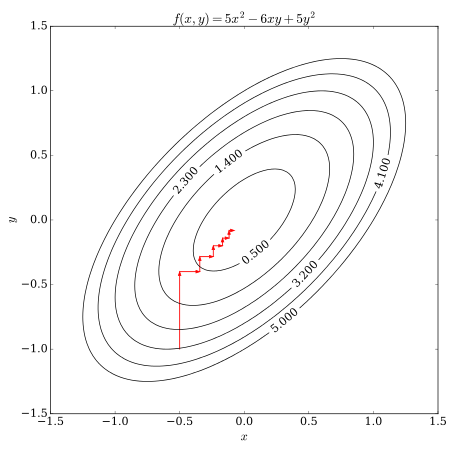
\includegraphics[scale=0.3]{pics/coordasc.png}
\end{center}

%Can be generalized in many ways:
%\begin{itemize}
%    \item Approximate $\argmax$
%    \[ a^{(i+1)} = a^{(i)} + \eta \nabla_a f(a^{(i)}, b^{(i)})\]
%    \item Block coordinate ascent
%\end{itemize}
\end{frame}

\begin{frame}
\thetitle{Preview}
\vspace{-4mm}
\begin{table}[]
    \centering
    \small
    \begin{tabular}{l c c c }
    \toprule
        Optimization Strategy  & $q$ &  $\max_\lambda$ & $\max_\theta$ \\
    \midrule
         Log Marginal Likelihood & - & - & Grad \\
         Expectation Maximization & Posterior & Bayes & Closed \\
         Variational EM &  Factored & Coord. & Closed \\
         Stochastic Variational EM  & Factored  & Grad & Grad\\
         Variational Autoencoder & Amortized & Grad & Grad \\
         \bottomrule
    \end{tabular}
\end{table}
\vspace{-2mm}
\textbf{$q$ Family examples} \\
Posterior: $q(z\param \lambda)$ matches $p(z \given x)$\\
Factored: e.g. $q(z^{(n)}) = \prod_{t} q(z^{(n)}_t\param \lambda^{(n)})$ \\
Amortized: e.g. $q(z^{(n)}) = \text{NN}(x^{(n)}\param \lambda)$  \\
\textbf{$\lambda$ Optimization Methods} \\
Bayes Rule: $q(z;\lambda) = p(z \given x )$ \\
Coordinate: $\lambda^{(n)*}_t = \argmax_{\lambda^{(n)}_t} \ELBO(\theta, \lambda^{(n)} \param x^{(n)}) $ \\
Gradient:\ $\lambda = \lambda + \eta \nabla_\lambda \ELBO(\theta, \lambda)$ \\
\end{frame}

\begin{frame}
\begin{tikzpicture}
% nodes
\node (dots) {$\ldots$};%
 \node[latent] (z) {$y^{(n)}$};%
 \node[const, right=of z] (x) {$x^{(n)}$};%
 %\node[obs, right=1cm of dots] (xT) {$x_T^{(n)}$};%
 \node[const, above=of z] (pi) {$\mathbf{w}$};
% plate
 \plate {plate1} {(z)(x)} {$N$}; %
 \edge{pi}{z};
 \edge{x}{z};
 
\end{tikzpicture}
    
\end{frame}

\begin{frame}{Frame Title}
    \begin{center}
\begin{tikzpicture}
% nodes
\node (dots) {$\ldots$};%
 \node[latent] (z) {$z^{(n)}$};%
 \node[const, right=of z] (x) {$x^{(n)}$};%

 %\node[obs, right=1cm of dots] (xT) {$x_T^{(n)}$};%
 \node[const, above=of z] (pi) {$\lambda$};
% plate
 \plate {plate1} {(z)(x)} {$N$}; %
 \edge{pi}{z};
 \edge{x}{z};
 
\end{tikzpicture}
\begin{tikzpicture}
% nodes
\node (dots) {$\ldots$};%
 \node[latent] (z) {$z^{(n)}$};%
 %\node[obs, right=1cm of dots] (xT) {$x_T^{(n)}$};%
 \node[const, above=of z] (pi) {$\lambda^{(n)}$};
% plate
 \plate {plate1} {(z)(pi)} {$N$}; %
 \edge{pi}{z};
\end{tikzpicture}
\begin{tikzpicture}
% nodes
\node (dots) {$\ldots$};%
 \node[latent] (z) {$z_1^{(n)}$};%
 \node[latent, right= of z] (zT) {$z_T^{(n)}$};%

 %\node[obs, right=1cm of dots] (xT) {$x_T^{(n)}$};%
 \node[const, above=of z] (pi) {$\lambda_1^{(n)}$};
\node[const, above=of zT] (piT) {$\lambda_T^{(n)}$};
%
% plate
 \plate {plate1} {(z)(pi)(piT)(zT)} {$N$}; %
 \edge{pi}{z};
 \edge{piT}{zT};
\end{tikzpicture}
\end{center}

\end{frame}

%\begin{frame}
%\thetitle{Optimization Strategy: Coordinate Ascent}
%\center
%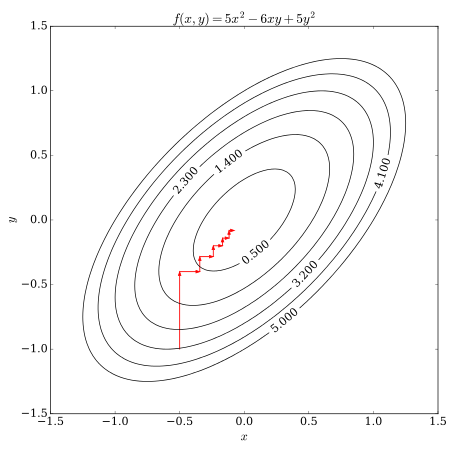
\includegraphics[scale=0.4]{pics/coordasc.png}
%\\
%(from {\footnotesize \url{https://en.wikipedia.org/wiki/Coordinate_descent}})
%\end{frame}

%\begin{frame}
%\thetitle{Coordinate Ascent on the ELBO}
%Aggregate ELBO
%\[ L(\theta, \lambda^{(1)}, \dots, \lambda^{(N)}) =  \sum_{n=1}^{N} \ELBO(\theta, \lambda^{(n)} \param x^{(n)}) \]
%Repeat:
%\begin{enumerate}
%\item \textbf{Inference Step}
%\[ L(\theta, \underbrace{\lambda^{(1)}, \dots, \lambda^{(N)}}_{\text{update}})  \]
%\item \textbf{Learning Step}
%\[ L(\underbrace{\theta}_{\text{update}}, \lambda^{(1)}, \dots, \lambda^{(N)}) \]
%\end{enumerate}
%\end{frame}

\begin{frame}
\thetitle{Coordinate Ascent on the ELBO: Step 1}
\vspace{-6mm}
\[ L(\theta, \lambda) =  \sum_{n=1}^{N} \ELBO(\theta, \lambda \param x^{(n)}) \]
\begin{enumerate}
    \item \textbf{Inference Step}: Since
    \begin{align*}
        \ELBO(\theta, \lambda^{} \param x^{}) = \log p(x^{} \param \theta) -
     \KL[q(z \param \lambda^{}) \Vert p(z \given x^{} \param \theta)]
    \end{align*} 
    This is equivalent to setting for all $n$
    \begin{align*}
        \lambda^{(n)} &= \argmax_{\lambda} \ELBO(\theta, \lambda ; x^{(n)}) \\
        &= \argmin_{\lambda} \KL[q(z \param \lambda) \Vert p(z \given x^{(n)} \param \theta)]
    \end{align*} 
\end{enumerate}
(the $\argmax$ operations may be approximate)
\end{frame}

\begin{frame}
\thetitle{Coordinate Ascent on the ELBO: Learning}
\vspace{-6mm}
\[ L(\underbrace{\theta}_{\text{update}}, \lambda^{(1)}, \dots, \lambda^{(N)}) =  \sum_{n=1}^{N} \ELBO(\theta, \lambda^{(n)}\param x^{(n)}) \]
\begin{enumerate}
 \setcounter{enumi}{1}
    \item \textbf{Learning Step}: Since
    \begin{align*}
        \ELBO(\theta, \lambda \param x) = \E_{q(z \param \lambda)}[\log p(x, z \param \theta) -\log q(z \param \lambda) ]
    \end{align*} 
    This is equivalent to
        \begin{align*}
            \theta^{} &= \argmax_\theta \sum_{n=1}^{N} \ELBO(\theta, \lambda^{(n)}\param x^{(n)}) \\
            &= \argmax_\theta \sum_{n=1}^N \E_{q(z \given \lambda^{(n)})}[\log p(x^{(n)}, z \param \theta)] 
        \end{align*} 
\end{enumerate}
(the $\argmax$ operation may also be approximate)
\end{frame}


\begin{frame}
\thetitle{Coordinate Ascent on the ELBO}
\begin{itemize}
    \item Since ELBO lower bounds log marginal likelihood, repeating inference/learning (i.e. coordinate ascent on the aggregate ELBO) will ideally learn $\theta$ that gives good log likelihood.
    \item The complete data likelihood $\log p(x, z\param \theta)$ is easy to evaluate, whereas $\log p(x \param \theta)$ may be hard.
\end{itemize}
\end{frame}



\subsection{Tractable Inference}
\begin{frame}
\begin{center}
\structure{Tractable Posterior Inference}
\end{center}
\begin{itemize}
    \item First consider cases where we can perform tractable posterior inference, i.e.
    \[ p(z \given x \param \theta) = \frac{p(x, z \param \theta)}{p(x \param \theta)}\]
    \item Equivalent marginal likelihood being tractable
    \[  p(x \param \theta) = \sum_{z} p(x, z \param \theta) \]
    \item Examples: Naive Bayes, Hidden Markov Models, Probabilistic Context Free Grammars
\end{itemize}
\end{frame}

\begin{frame}
\begin{center}
\structure{EM as Coordinate Ascent}
\end{center}
Randomly initialize $\theta^{(0)}$. Then repeat for $i$
\begin{enumerate}
    \item \textbf{Inference Step}: For all $n$
    \begin{align*}
        \lambda^{(n)} &= \argmin_{\lambda} \KL[q(z \param \lambda) \Vert p(z \given x^{(n)} \param \theta^{(i)})]
    \end{align*} 
\end{enumerate}
\begin{itemize}
    \item This is minimized by setting $q(z \param \lambda^{(n)}) = p(z \given x^{(n)} \param \theta^{(i)})$, which we assumed was tractable. 
    \item Corresponds to the E-step in the Expectation Maximization algorithm \citep{dempster77em}.
\end{itemize}

\end{frame}

\begin{frame}
\begin{center}
\structure{EM as Coordinate Ascent}
\end{center}

\begin{enumerate}
 \setcounter{enumi}{1}
    \item \textbf{Learning Step} (exact): 
        \begin{align*}
            \theta^{(i+1)} 
            &= \argmax_\theta \sum_{n=1}^N \E_{q(z \given \lambda^{(n)})}[\log p(x^{(n)}, z \param \theta^{})]  \\
            &= \argmax_\theta \sum_{n=1}^N \E_{p(z \given x^{(n)} \param \theta^{(i)})}[\log p(x^{(n)}, z \param \theta)] 
        \end{align*} 
\end{enumerate}
\begin{itemize}
    \item This corresponds the M-step in EM.
\end{itemize}
\end{frame}

\begin{frame}
\thetitle{Recap}
\vspace{-3mm}
\begin{table}[]
    \centering
    \begin{tabular}{l c c }
    \toprule
        Optimization Method  & Inference & Learning \\
    \midrule
         Expectation Maximization & Exact Post. & Exact \\
         {\color{white} Log Marginal Likelihood} & {\color{white} Exact Post.} & {\color{white} Gradient} \\
         {\color{white} Variational EM} & {\color{white} VI} & {\color{white} Exact/Gradient} \\
         {\color{white} Stochastic Variational EM} & {\color{white} SVI} & {\color{white} Gradient}\\
         {\color{white} Variational Autoencoder} & {\color{white} AVI} & {\color{white} Gradient} \\
         \bottomrule
    \end{tabular}
\end{table}
\end{frame}

\begin{frame}
\begin{center}
\structure{Generalized EM}
\end{center}
What if it is not possible to perform the M-step exactly?
\begin{enumerate}
 \setcounter{enumi}{1}
    \item \textbf{Learning Step} (gradient): 
        \begin{align*}
            \theta^{(i+1)} &= \theta^{(i)} + \eta \nabla_\theta Q(\theta)
        \end{align*} 
        \begin{align*}
            \nabla_\theta Q(\theta) &=\nabla_\theta \Big (\sum_{n=1}^N \E_{p(z \given x^{(n)} \param \theta^{(i)})}[\log p(x^{(n)}, z \param \theta)] \Big) \\
            &=\sum_{n=1}^N \E_{p(z \given x^{(n)} \param \theta^{(i)})}[\nabla_\theta \log p(x^{(n)}, z \param \theta)]
        \end{align*}
\end{enumerate}
\begin{itemize}
    \item Sometimes referred to as \textbf{generalized EM} \citep{neal1998,Murphy:2012:MLP:2380985}
\end{itemize}
\end{frame}

\begin{frame}
\begin{center}
\structure{Interlude: Gradient Ascent on Log Marginal Likelihood}
\end{center}
Define the data log marginal likelihood as 
\[ M(\theta) = \sum_{n=1}^N \log p(x^{(n)} \param \theta) = \sum_{n=1}^N \log \sum_z p(x^{(n)}, z \param \theta)  \]

\begin{itemize}
    \item Why not perform gradient ascent directly on $M(\theta)$?
    \item Claim: generalized EM (i.e. exact E-step, gradient-based M-step) is equivalent to 
    performing gradient ascent directly on the log marginal likelihood.
\end{itemize}
\end{frame}


\begin{frame}
\begin{center}
\structure{Gradient Ascent on Log Marginal Likelihood}
\end{center}
\vspace{-3mm}
Gradient for a single point
\begin{align*}
    \nabla_\theta \log p(x \param \theta) &= \nabla_\theta \log \sum_{z} p(x, z \param \theta)  \\
    &= \frac{1}{\sum_{z}p(x, z \param \theta)}\nabla_\theta \sum_{z} p(x,z \param \theta) \\
    &= \frac{1}{p(x \param \theta)} \sum_{z} p(x,z \param \theta) \nabla_\theta \log p(x, z \param \theta) \\
        &= \sum_{z}   \frac{p(x,z \param \theta)}{p(x \param \theta)} \nabla_\theta \log p(x, z \param \theta) \\
        &=  \sum_{z} p(z \given x \param \theta) \nabla_\theta \log p(x, z \param \theta) \\
        &= \E_{p(z \given x \param \theta)} [\nabla_\theta \log p(x, z \param \theta)]
\end{align*} 
\end{frame}

\begin{frame}
\begin{center}
\structure{Gradient Ascent on Log Marginal Likelihood}
\end{center}
\vspace{-3mm}
Therefore
\begin{align*}
    \nabla_\theta M(\theta) &= \sum_{n=1}^N  \nabla_\theta \log p(x^{(n)} \param \theta) \\
    &= \sum_{n=1}^N \E_{p(z \given x^{(n)} \param \theta)} [\nabla_\theta \log p(x^{(n)}, z \param \theta)] \\
    &= \nabla_\theta Q(\theta)
\end{align*} 
\end{frame}

\begin{frame}
\begin{center}
\structure{Gradient Ascent on Log Marginal Likelihood}
\end{center}
    \vspace{-2mm}
\begin{itemize}
    \item EM with gradient-based M-step is equivalent to directly performing gradient ascent on the log marginal likelihood \citep{salak2003,kirk2010}.
    \item Practically, this means we don't have to manually perform posterior inference in the E-step. Can just calculate $\log p(x \param \theta)$ and call backpropagation.
    \item Example: in PCFGs with neural parameterization of rule probabilities, just implement inside algorithm to calculate $\log p(x \param \theta)$ and backpropagate using autodiff. No need to implement outside algorithm. 
\end{itemize}
    \vspace{2mm}
    (See \cite{eisner2016}:  ``Inside-Outside and Forward-Backward Algorithms Are Just Backprop")
\end{frame}


\begin{frame}
\thetitle{Recap}
\vspace{-3mm}
\begin{table}[]
    \centering
    \begin{tabular}{l c c }
    \toprule
        Optimization Method  & Inference & Learning \\
    \midrule
         Expectation Maximization & Exact Post. & Exact \\
          Log Marginal Likelihood & Exact Post. &  Gradient \\
         {\color{white} Variational EM} & {\color{white} VI} & {\color{white} Exact/Gradient} \\
         {\color{white} Stochastic Variational EM} & {\color{white} SVI} & {\color{white} Gradient}\\
         {\color{white} Variational Autoencoder} & {\color{white} AVI} & {\color{white} Gradient} \\
         \bottomrule
    \end{tabular}
\end{table}
\end{frame}

\subsection{Intractable Inference}

\begin{frame}
\begin{center}
\structure{Intractable Case}
\end{center}
\begin{itemize}
    \item Previously we have assumed that calculating $p(z \given x \param \theta)$ is tractable, leading to an exact inference step
    \[ \argmin \KL[q(z \param \lambda^{}) \Vert p( z \given x \param \theta)]\]
    \item Not the case in general, e.g.:
     \begin{align*}
         z \sim \mathcal{N}(0, I) && x \sim p(x \given z \param \theta)
     \end{align*}
     \item If likelihood $p(x \given z \param \theta)$ parameterized with a deep model, prior      is (generally) not conjugate to the likelihood $\implies$ 
    \[ p(z \given x \param \theta) = \int p(x \given z \param \theta) p(z) dz \] 
    is intractable.
\end{itemize}
\end{frame}
\begin{frame}
\thetitle{Variational Inference \citep{Jordan1999}}
\begin{itemize}
\item \textbf{Idea:} Restrict the family of distributions $q$.
Depending on choice of family, \textbf{approximate} inference may be tractable.
\item $q(z \param \lambda)$ is called a \textbf{variational distribution}, and 
\[ \mathcal{Q} = \{ q(z \param \lambda)\} \] 
(i.e. collection of variational distributions) is called the \textbf{variational family}.
\item Example: \\
$q(z \param \lambda) = \mathcal{N}(\mu, \sigma^2)$, $\lambda = [\mu, \sigma]$ \\
$\mathcal{Q}$: all Gaussian distributions.
\end{itemize}
\end{frame}

\begin{frame}
\thetitle{Variational Inference \citep{Jordan1999}}
\begin{itemize}
    \item Previously:
    \[ \argmin_\lambda \KL [q(z \param \lambda) \Vert p(z \given x \param \theta)]\]
    \item Now:
    \[ \argmin_{\lambda : q(z\param \lambda) \in \mathcal{Q}} \KL [q(z \param \lambda) \Vert p(z \given x \param \theta)]\]
\end{itemize}
Variational inference turns an inference problem into an optimization problem.
\end{frame}

\begin{frame}
\thetitle{Variational Inference \citep{Jordan1999}}
$\mathcal{D}$: All distributions over $z$ \\
\color{white}{$\mathcal{Q}$: Variational family }
\center
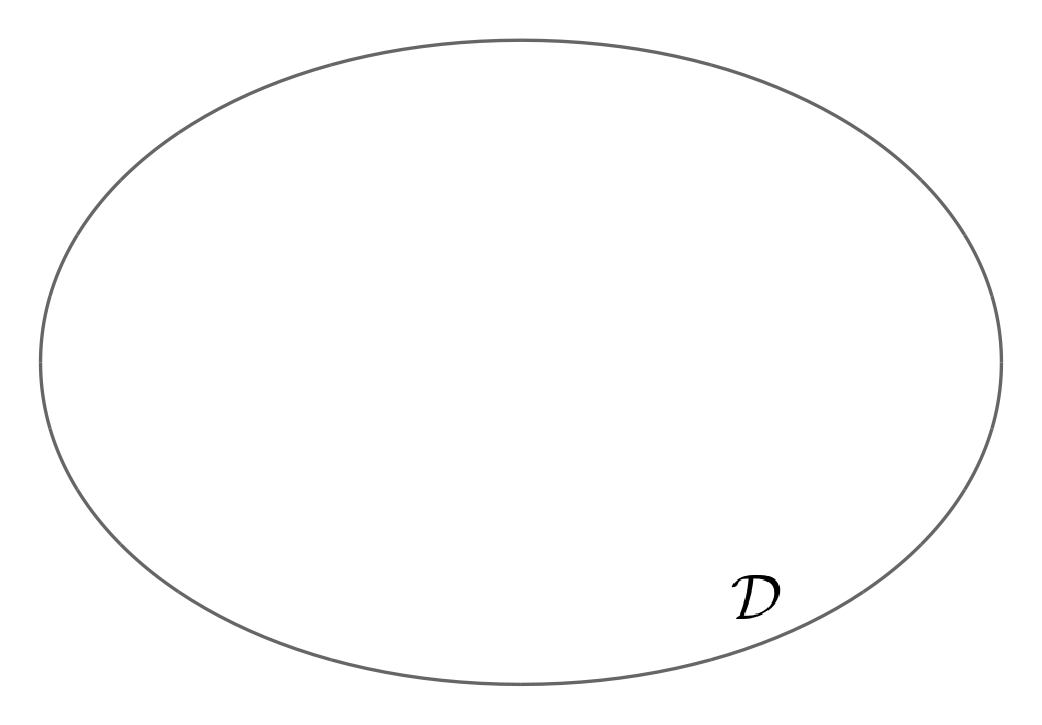
\includegraphics[scale=0.26]{pics/vi1.png}
\end{frame}

\begin{frame}
\thetitle{Variational Inference \citep{Jordan1999}}
$\mathcal{D}$: All distributions over $z$ \\
\color{white}{$\mathcal{Q}$: Variational family }
\center
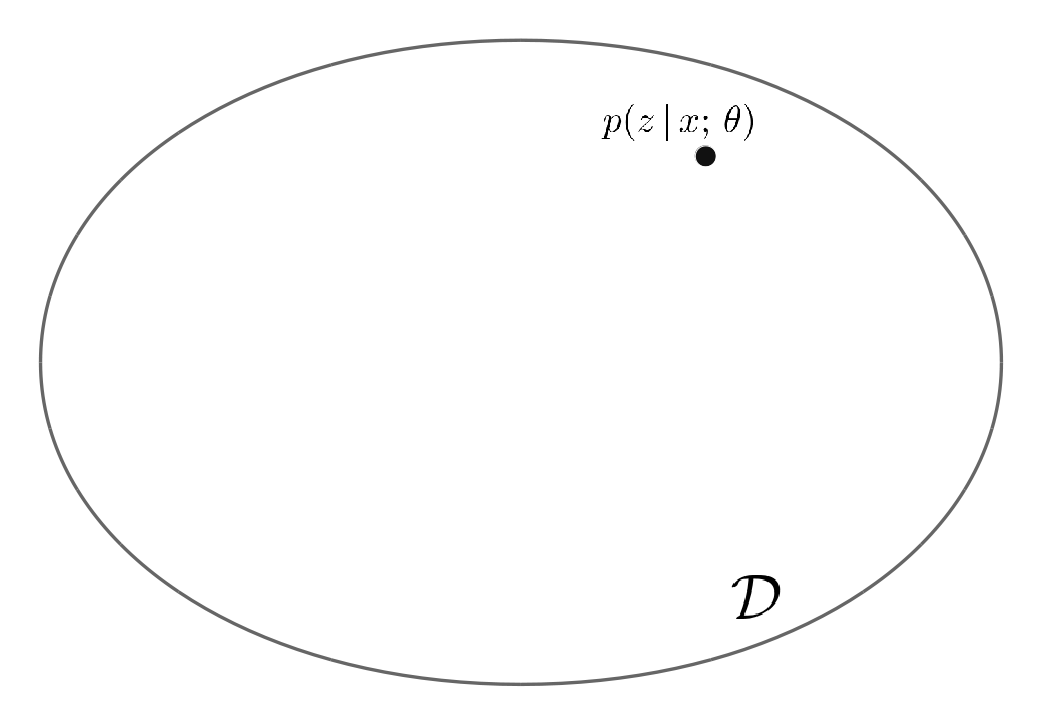
\includegraphics[scale=0.26]{pics/vi2.png}
\end{frame}

\begin{frame}
\thetitle{Variational Inference \citep{Jordan1999}}
$\mathcal{D}$: All distributions over $z$ \\
$\mathcal{Q}$: Variational family 
\center
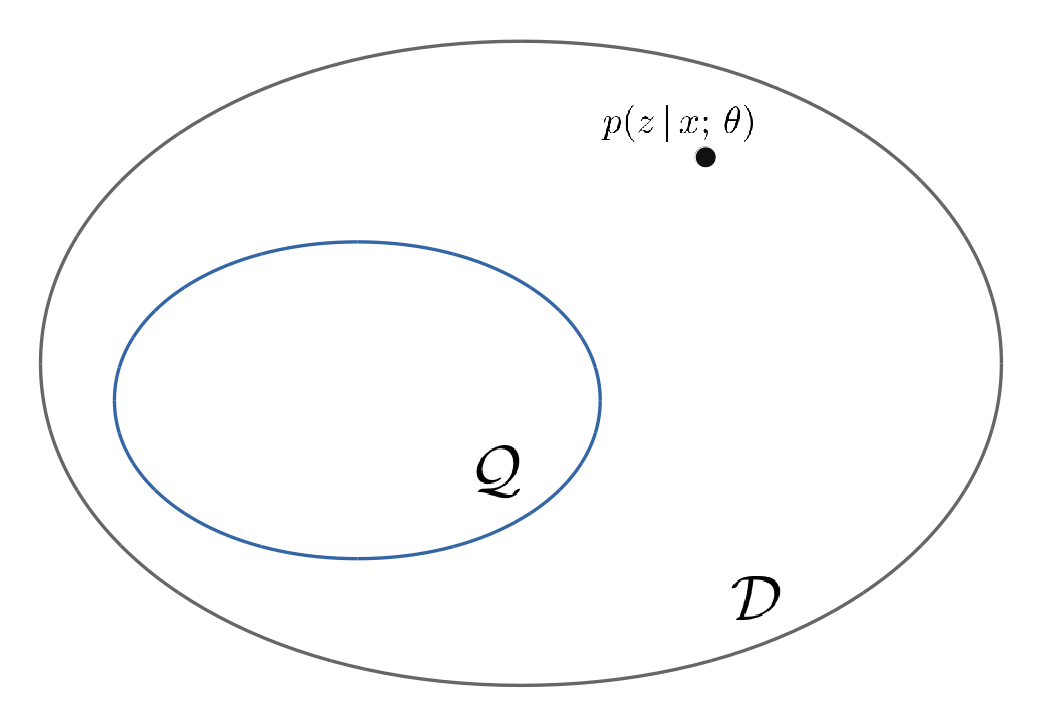
\includegraphics[scale=0.26]{pics/vi3.png}
\end{frame}

\begin{frame}
\thetitle{Variational Inference \citep{Jordan1999}}
$\mathcal{D}$: All distributions over $z$ \\
$\mathcal{Q}$: Variational family 
\center
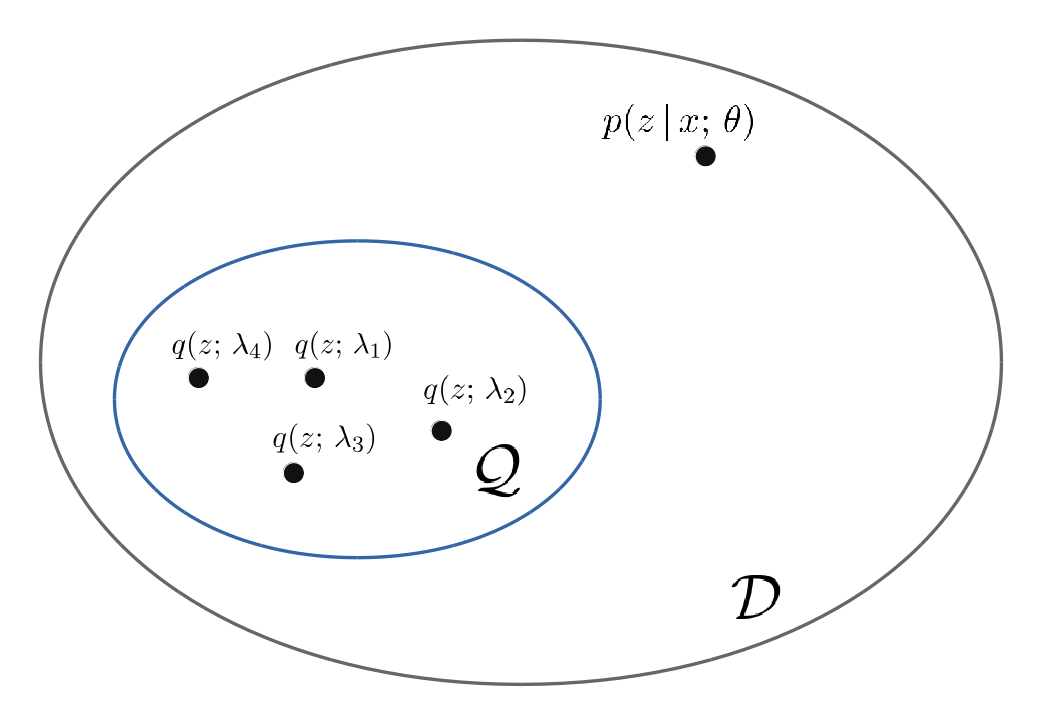
\includegraphics[scale=0.26]{pics/vi4.png}
\end{frame}

\begin{frame}
\thetitle{Variational Inference \citep{Jordan1999}}
$\mathcal{D}$: All distributions over $z$ \\
$\mathcal{Q}$: Variational family 
\center
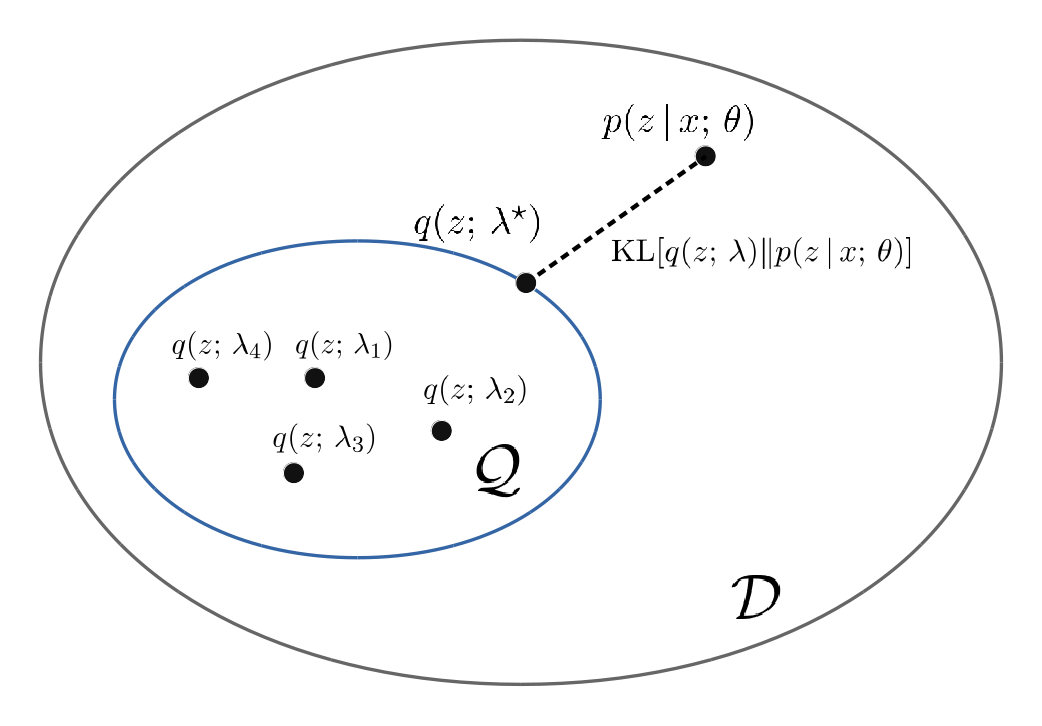
\includegraphics[scale=0.26]{pics/vi5.png}
\end{frame}


\begin{frame}
\thetitle{Variational EM \citep{neal1998}}
Assume for now we can efficiently minimize $\KL [q(z \param \lambda) \Vert p(z \given x^{(n)} \param \theta)]$ for each $x^{(n)}$

\begin{enumerate}
    \item Inference Step: For $n = 1, \dots, N$, calculate the approximate posterior $q(z  \param \lambda^{(n)})$ keeping $\theta^{(i)}$ fixed
    \[ \lambda^{(n)} = \argmin_{\lambda: q(z \param \lambda) \in \mathcal{Q}} \KL [q(z \param \lambda) \Vert p(z \given x^{(n)} \param \theta^{(i)})]\]
    \item Learning Step: Keeping $\lambda^{(n)}$'s fixed, maximize the expected complete data likelihood 
    \[ \theta^{(i+1)} = \argmax_{\theta} \sum_{n=1}^N \E_{q(z \param \lambda^{(n)})}[\log p(x, z \param \theta)] \]
    (can also approximately maximize)
\end{enumerate}
\end{frame}

\begin{frame}
\thetitle{Recap}
\vspace{-3mm}
\begin{table}[]
    \centering
    \begin{tabular}{l c c }
    \toprule
        Optimization Method  & Inference & Learning \\
    \midrule
         Expectation Maximization & Exact Post. & Exact \\
         Log Marginal Likelihood & Exact Post. & Gradient \\
         Variational EM & VI & Exact/Gradient \\
         {\color{white} Stochastic Variational EM} & {\color{white} SVI} & {\color{white} Gradient}\\
         {\color{white} Variational Autoencoder} & {\color{white} AVI} & {\color{white} Gradient} \\
         \bottomrule
    \end{tabular}
\end{table}
\end{frame}


\begin{frame}
\thetitle{Stochastic Variational Inference \citep{Hoffman2013}}
\begin{itemize}
    \item Exact variational inference 
\[ \lambda^{(n)} = \argmin_{\lambda : q(z \param \lambda) \in \mathcal{Q}} \KL[q(z \param \lambda)  \, \Vert \, p(z \given x^{(n)} \param \theta)]\]
could be expensive/slow.
\item Stochastic variational inference (SVI): approximately minimize KL with (for example) gradient descent.
\item Approximate approximate inference.
\end{itemize}
\end{frame}

\begin{frame}
\thetitle{Stochastic Variational Inference \citep{Hoffman2013}}

\textbf{Stochastic Variational EM}
\begin{enumerate}
    \item Randomly initialize $\lambda^{(n)}_0$ for all $n$ (usually over mini-batch)
    \item $K$-steps of gradient descent for each $x^{(n)}$
    \[ \lambda_{k}^{(n)} = \lambda_{k-1}^{(n)} + \eta \nabla_\lambda \ELBO(\theta^{(i)}, \lambda^{(n)}_{k-1} \param x^{(n)}) \]
    \item Update $\theta$
    \[ \theta^{(i+1)} = \theta^{(i)} + \eta \sum_{n=1}^N \nabla_\theta \ELBO(\theta^{(i)}, \lambda^{(n)}_K \param x^{(n)}) \]
\end{enumerate}
\end{frame}

\begin{frame}
\thetitle{Recap}
\vspace{-3mm}
\begin{table}[]
    \centering
    \begin{tabular}{l c c }
    \toprule
        Optimization Method  & Inference & Learning \\
    \midrule
         Expectation Maximization & Exact Post. & Exact \\
         Log Marginal Likelihood & Exact Post. & Gradient \\
         Variational EM & VI & Exact/Gradient \\
         Stochastic Variational EM & SVI &  Gradient\\
         {\color{white} Variational Autoencoder} & {\color{white} AVI} & {\color{white} Gradient} \\
         \bottomrule
    \end{tabular}
\end{table}
\end{frame}

\begin{frame}
\thetitle{Amortized Variational Inference \citep{Kingma2014}}
\begin{itemize}
    \item SVI allows for faster inference since we can approximately perform VI with 
    gradient ascent.
    \item But this could still be too slow, since each SVI step requires calculating the gradient $ \nabla_\lambda \ELBO(\theta^{(i)}, \lambda^{(n)}_{k-1} \param x^{(n)})$ for each data point.
    \item Amortized Variational Inference: \\
    \textbf{Predict} the variational parameters from a parametric function over $x$
\end{itemize}
\end{frame}

\begin{frame}
\thetitle{Amortized Variational Inference \citep{Kingma2014}}
Define an \textbf{inference network} parameterized by $\phi$. Variational parameters for each data point
are given by
\[ \lambda^{(n)} = \enc(x^{(n)} \param \phi)\]
\begin{itemize}
    \item $\phi$ trained via SGD to perform inference
    \[ \phi = \phi + \eta \nabla_\phi \sum_{n=1}^B \ELBO(\theta, \enc(x^{(n)} \param \phi) \param x^{(n)})\]
    \item Since a \textbf{global} inference network $\phi$ is used for all $x^{(n)}$, we say that the approximate posterior inference procedure is \textbf{amortized} across the dataset.
\end{itemize}
\end{frame}

\begin{frame}
\thetitle{Amortized Variational Inference \citep{Kingma2014}}
$\mathcal{D}$: All distributions over $z$ \\
$\mathcal{Q}$: Variational family \\
{\color{white} $\mathcal{Q}_\phi$: Amortized Variational family }
\center
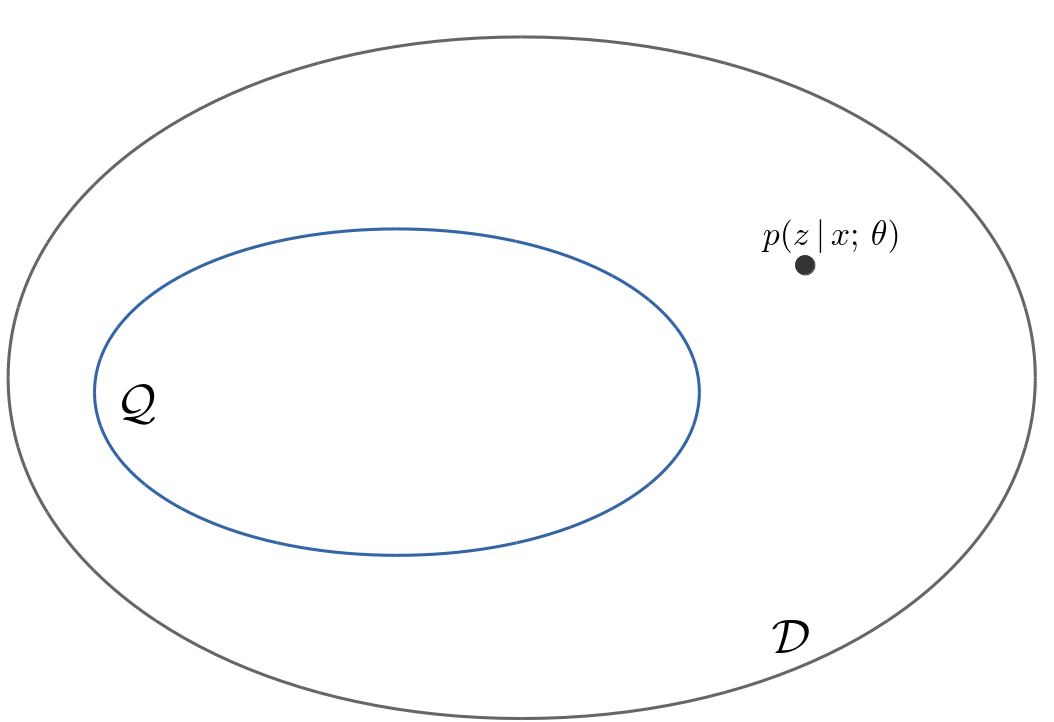
\includegraphics[scale=0.24]{pics/avi1.png}
\end{frame}
 
 
\begin{frame}
\thetitle{Amortized Variational Inference \citep{Kingma2014}}
$\mathcal{D}$: All distributions over $z$ \\
$\mathcal{Q}$: Variational family \\
{\color{white} $\mathcal{Q}_\phi$: Amortized Variational family }
\center
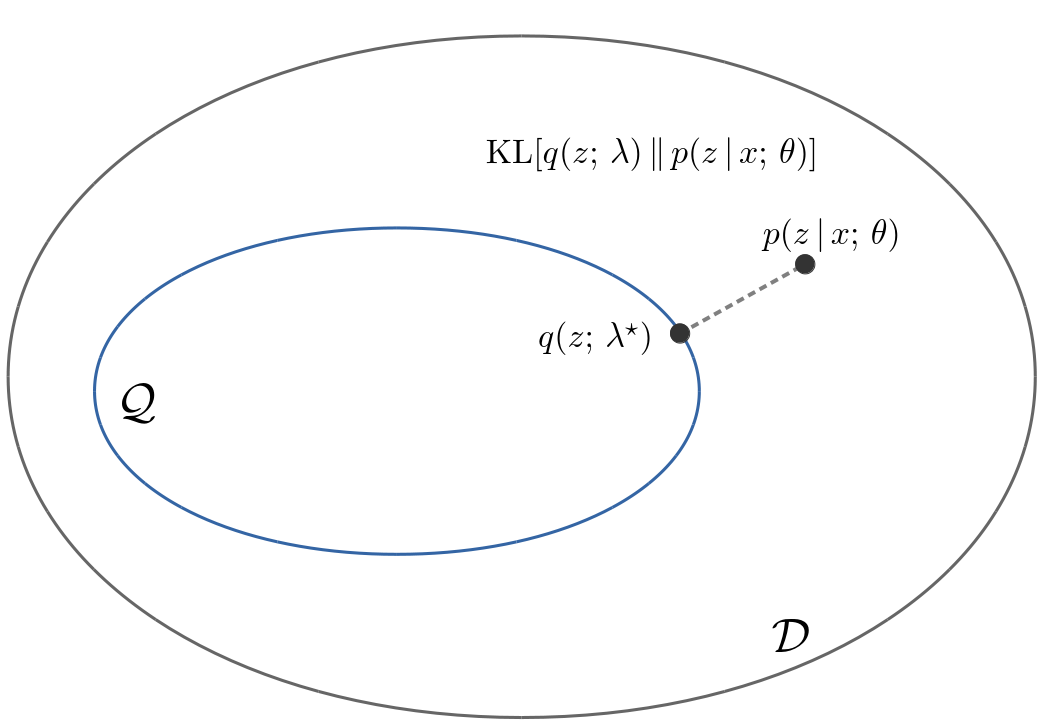
\includegraphics[scale=0.24]{pics/avi2.png}
\end{frame}
 
\begin{frame}
\thetitle{Amortized Variational Inference \citep{Kingma2014}}
$\mathcal{D}$: All distributions over $z$ \\
$\mathcal{Q}$: Variational family \\
$\mathcal{Q}_\phi$: Amortized Variational family 
\center
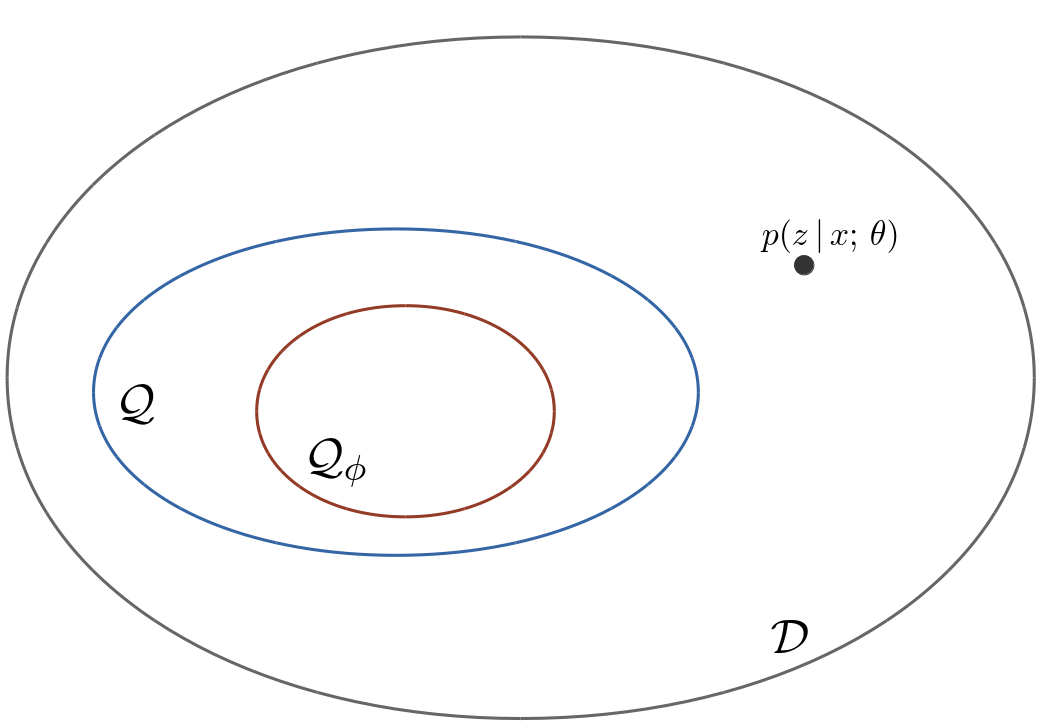
\includegraphics[scale=0.24]{pics/avi3.png}
\end{frame}
  
\begin{frame}
\thetitle{Amortized Variational Inference \citep{Kingma2014}}
$\mathcal{D}$: All distributions over $z$ \\
$\mathcal{Q}$: Variational family \\
$\mathcal{Q}_\phi$: Amortized Variational family 
\center
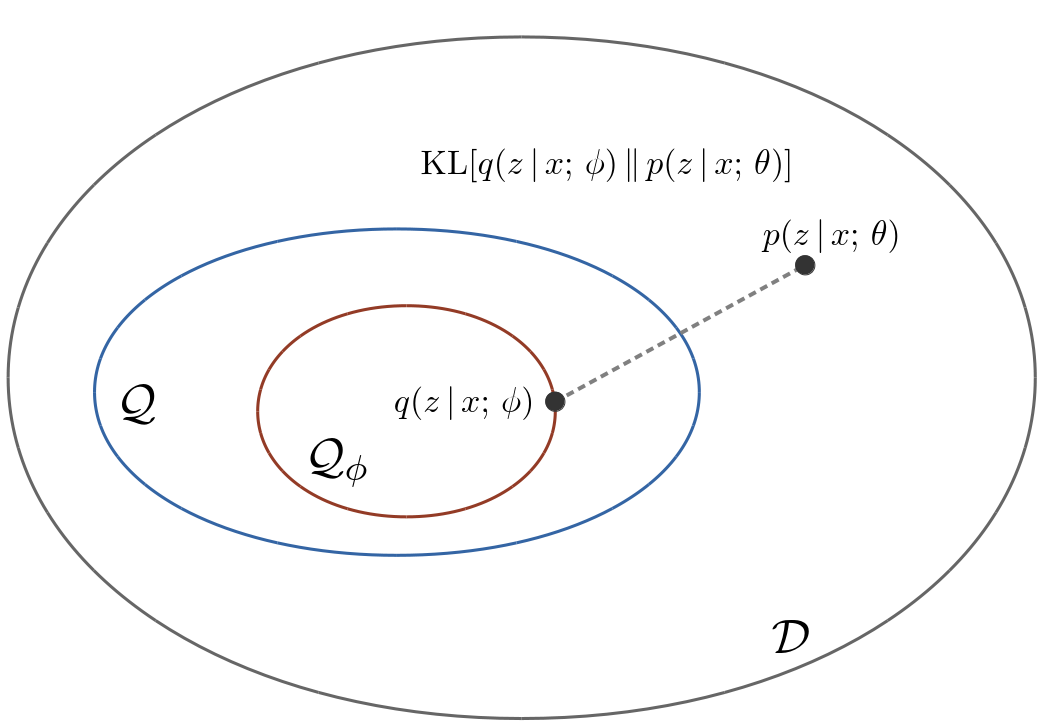
\includegraphics[scale=0.24]{pics/avi4.png}
\end{frame}

 
\begin{frame}
\thetitle{Variational Autoencoders \citep{Kingma2014}}
\begin{itemize}
    \item Deep generative models trained with amortized inference
    \item Generative model $\theta$ and inference network $\phi$ trained \textbf{jointly} to maximize the aggregate ELBO
    \[L(\theta, \phi) =  \sum_{n=1}^N \ELBO(\theta, \phi \param x^{(n)})\]
    \item Typically trained with gradient-based optimization over mini-batches
    \begin{align*}
        \theta &= \theta + \eta \nabla_\theta L(\theta, \phi) \\
        \phi &= \phi + \eta \nabla_\phi L(\theta, \phi)
    \end{align*}
\end{itemize}
\end{frame}

\begin{frame}
\thetitle{Why ``autoencoder"?}
\begin{align*}
    &\ELBO(\theta, \phi \param x ) = \E_{q(z \given x \param \phi)}\Big[\log \frac{p(x, z \param \theta)}{q(z \given x \param \phi)}\Big] \\
    &= \E_{q(z \given x \param \phi)}[\log p( x \given z \param \theta) + \log p(z) - \log q(z \given x \param \phi)] \\
        &= \E_{q(z \given x \param \phi)}[\log p( x \given z \param \theta)] - \E_{q(z \given x \param \phi)}\Big[\log \frac{q(z \given x \param \phi)}{p(z)} \Big] \\
        &= \E_{q(z \given x \param \phi)}[\log p( x \given z \param \theta)] - \KL[q(z \given x \param \phi) \Vert p(z)]
\end{align*}
\end{frame}


\begin{frame}
\thetitle{Why ``autoencoder"?}
\begin{align*}
    &\ELBO(\theta, \phi \param x )  = \E_{q(z \given x \param \phi)}\Big[\log \frac{p(x, z \param \theta)}{q(z \given x \param \phi)}\Big] \\
    &= \E_{q(z \given x \param \phi)}[\log p( x \given z \param \theta) + \log p(z) - \log q(z \given x \param \phi)] \\
        &= \E_{q(z \given x \param \phi)}[\log p( x \given z \param \theta)] - \E_{q(z \given x \param \phi)}\Big[\log \frac{q(z \given x \param \phi)}{p(z)} \Big] \\
        &= \underbrace{\E_{q(z \given x \param \phi)}[\log p( x \given z \param \theta)]}_{\text{AE reconstruction likelihood}} - \underbrace{\KL[q(z \given x \param \phi) \Vert p(z)]}_{\text{Regularize posterior to prior}}
\end{align*}
\end{frame}


\begin{frame}
\thetitle{Recap}

\begin{table}[]
    \centering
    \begin{tabular}{l c c }
    \toprule
        Optimization Method  & Inference & Learning \\
    \midrule
         Expectation Maximization & Exact Post. & Exact \\
         Log Marginal Likelihood & Exact Post. & Gradient \\
         Variational EM & VI & Exact/Gradient \\
         Stochastic Variational EM & SVI & Gradient\\
         Variational Autoencoder & AVI & Gradient \\
         \bottomrule
    \end{tabular}
\end{table}
\vspace{-3mm}
\textbf{Inference Methods} \\
Exact Posterior: $q(z \param \lambda ) = p(z \given x \param \theta)$ \\
Variational Inference (VI): $\lambda = \argmax_\lambda \ELBO(\theta, \lambda \param x) $ \\
%=\min_\lambda \KL[q(z \param \lambda) \Vert p(z \given x \param \theta)]$ \\
Stochastic VI: $\lambda = \lambda + \eta \nabla_\lambda \ELBO(\theta, \lambda \param x)$ \\
Amortized VI: $\lambda = \enc(x \param \phi) $
\end{frame}

% 

\begin{frame}
\thetitle{Advanced Topics}
\begin{enumerate}
\item Gumbel-Softmax: Extend reparameterization to discrete variables.
\item Flows: Optimize a tighter bound by making $q$ more flexible.
\item Importance Weighted AE:  Optimize a tighter bound through importance sampling.
\end{enumerate}
\end{frame}

\subsection{Gumbel-Softmax}
\begin{frame}
\thetitle{Gumbel-Softmax \citep{Jang2017,Maddison2017}}
\begin{itemize}
    \item Recall the reparameterization trick for estimating $\nabla_\lambda \ELBO(\theta, \lambda \param x)$ in the continuous case.
    \item What if $z$ is discrete?
\end{itemize}
\end{frame}

\begin{frame}
\thetitle{Gumbel-Softmax \citep{Jang2017,Maddison2017}}
Review: we can always use score function estimator 
\begin{align*}
 \nabla_\lambda &\ELBO(x, \theta, \lambda) = \E_{q}\Big[\log \frac{p(x, z \param \theta)}{q(z \given x \param \lambda)}\nabla_{\lambda}\log q(z \given x \param \lambda)\Big]     \\
 &= \E_{q}\Big[\Big(\log \frac{p(x, z \param \theta)}{q(z \given x \param \lambda)}- B\Big)\nabla_{\lambda}\log q(z \given x \param \lambda)\Big] 
\end{align*}

\begin{itemize}
    \item Control variate $B$ (not dependendent on $z$, but can depend on $x$). 
    \item Estimate this quantity with another neural net \citep{Mnih2014}
    \[ \Big( B(x \param \psi) -\log \frac{p(x, z \param \theta)}{q(z \given x \param \lambda)} \Big)^2 \]
    \item Can we leverage the reparameterization trick instead?
\end{itemize}
\end{frame}

\begin{frame}
\thetitle{Gumbel-Softmax \citep{Jang2017,Maddison2017}}
The ``Gumbel-Max" trick \citep{Papandreou2011}
\[ p(z_k = 1 \param \alpha) = \frac{\alpha_k}{\sum_{j=1}^K \alpha_j} \]
where $z = [0, 0, \dots, 1 , \dots, 0]$ is a one-hot vector.
Can sample from $p(z \param \alpha)$ by
\begin{enumerate}
    \item Drawing independent Gumbel noise $\epsilon =  \epsilon_1, \dots, \epsilon_K$
    \[ \epsilon_k = -\log (- \log u_k) \,\,\,\,\,\,\,\,\,\,\,\,\, u_k \sim \mathcal{U}(0, 1)\]
    \item Adding $\epsilon_k$ to $\log \alpha_k$, finding argmax, i.e.
    \[ i = \argmax_k [\log \alpha_k + \epsilon_k] \,\,\,\,\,\,\,\,\,\,\,\,\,\,\,
    z_i = 1 \]

\end{enumerate}
    More succinctly,
    \[ z = \argmax_{s \in \Delta^{K-1}}  \,\,(\log \alpha + \epsilon)^\top s = g(\epsilon, \alpha) \]
    
\end{frame}

\begin{frame}
\thetitle{Gumbel-Softmax \citep{Jang2017,Maddison2017}}
So we can reparameterize, since $z = g(\epsilon, \alpha)$ is a deterministic function applied to stochastic noise. \\ Let's try applying this:
\[ q(z_k = 1 \given x \param \lambda) = \frac{\alpha_k}{\sum_{j=1}^K \alpha_j} \,\,\,\,\,\,\,\, \alpha = \enc(x \param \lambda) \]
\begin{align*}
    \nabla_\lambda \E_{q(z \given x \param \lambda)}\Big[& \log \frac{p(x, z \param \theta)}{q(z \given x \param \lambda)}\Big] \\ &= 
    \nabla_\lambda \E_{\epsilon \sim \text{Gumbel}}\Big[ \log \frac{ p(x, g(\epsilon, \alpha) \param \theta)}{q(g(\epsilon, \alpha) \given x \param \lambda)}\Big] \\
    &=      \E_{\epsilon \sim \text{Gumbel}}\Big[\nabla_\lambda \log \frac{ p(x, g(\epsilon, \alpha) \param \theta)}{q(g(\epsilon, \alpha) \given x \param \lambda)}\Big]
\end{align*}
\end{frame}

\begin{frame}
\thetitle{Gumbel-Softmax \citep{Jang2017,Maddison2017}}
But this won't work, since
\[ z = g(\epsilon, \alpha) = \argmax_{s \in \Delta^{K-1}} (\log \alpha + \epsilon)^\top s \]
has zero gradients almost everywhere.
\\ \vspace{3mm}
Gumbel-Softmax trick: replace $\argmax$ with $\softmax$
\[ z = \softmax((\log \alpha + \epsilon)/\tau) \]
i.e.
\[ z_k = \frac{\exp((\log \alpha_k + \epsilon_k)/\tau)}{\sum_{j=1}^K \exp ((\log \alpha_j + \epsilon_j)/\tau)}\]
where $\tau$ is a temperature term. 
\end{frame}

\begin{frame}
\thetitle{Gumbel-Softmax \citep{Jang2017,Maddison2017}}
\begin{itemize}
    \item Approaches a discrete distributution as $\tau \to 0$
    \item Reparameterizable by construction
    \item Differentiable and has non-zero gradients
\end{itemize}
\center
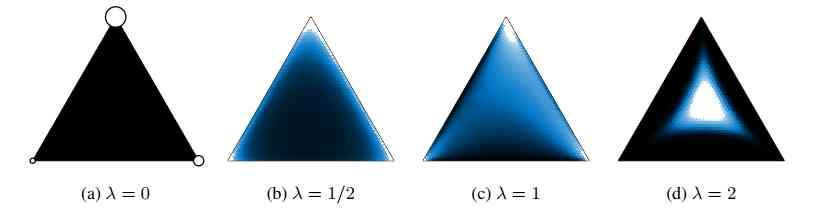
\includegraphics[scale=0.3]{pics/concrete.jpg} \\
(from \cite{Maddison2017})
\end{frame}

\begin{frame}
\thetitle{Gumbel-Softmax \citep{Jang2017,Maddison2017}}
\vspace{-5mm}
\begin{align*} 
  \nabla_\lambda& \E_{q(z \given x \param \lambda)}\Big[ \log \frac{p(x, z \param \theta)}{q(z \given x \param \lambda)}\Big] \\ &\approx 
\E_{ \epsilon \sim \text{Gumbel}}\Big[\nabla_\lambda \log \frac{ p(x, \softmax((\log \alpha + \epsilon)/\tau) \param \theta)}{q(\softmax((\log \alpha + \epsilon)/\tau) \given x \param \lambda)}\Big] 
\end{align*}
(anneal $\tau$ during training)
\begin{itemize}
\item See \cite{Maddison2017} on whether we can use the original categorical densities $p(z), q(z)$, or need to use relaxed densities $p_{\text{GS}}(z), q_{\text{GS}}(z)$.
\item Requires that $p(x \given z \param \theta)$ ``makes sense" for non-discrete $z$ (e.g. attention).
    \item Lower-variance, but biased gradient estimator. Variance $\to \infty$ as $\tau \to 0$.
\end{itemize}
\end{frame}

\subsection{Flows}

\begin{frame}
\thetitle{Flows \citep{Rezende2015,Kingma2016}}
Recall
\[ \log p(x \param \theta)  = \ELBO(\theta, \lambda; x) - \KL[q(z \given x \param \lambda)  \, \Vert \, p(z \given x \param \theta)]  \]
Bound is tight when variational posterior equals true posterior
\[ q(z \given x \param \lambda) = p(z \given x \param \theta) \implies \log p(x \param \theta) = \ELBO( \theta,  \lambda \param x) \]
We want to make $q(z \given x \param \lambda)$ as flexible as possible:
can we do better than just Gaussian?
\end{frame} 

\begin{frame}
\thetitle{Flows \citep{Rezende2015,Kingma2016}}
\textbf{Idea:} transform a sample from a simple initial variational distribution, 
\[ z_0 \sim q(z \given x \param \lambda) = \mathcal{N}(\mu, \sigma^2) \,\,\,\,\,\,\,\,\,\,\,\,\,\, \mu, \sigma^2 = \enc(x \param \lambda)\]
into a more complex one
\[ z_K = f_K \circ \dots \circ f_2 \circ f_1(z_0 \param \lambda)\]
where $f_i(z_{i-1}\param \lambda)$'s are \textbf{invertible} transformations (whose parameters are
absorbed by $\lambda$).
\end{frame} 


\begin{frame}
\thetitle{Flows \citep{Rezende2015,Kingma2016}}
Sample from final variational posterior is given by $z_K$. By the change of variables formula
\begin{align*}
\log q_K(z_K \given &x \param \lambda) = \log q(z_0 \given x \param \lambda) + 
\sum_{k=1}^K \log \Big | \frac{\partial f_k^{-1}}{\partial z_{k}}\Big |  \\
&=\underbrace{\log q(z_0 \given x \param \lambda)}_{\text{log density of Gaussian}} - 
\sum_{k=1}^K \underbrace{\log \Big | \frac{\partial f_k}{\partial z_{k-1}}\Big |}_{\text{log determinant of Jacobian}} 
\end{align*}
\\
\vspace{5mm}
Determinant calculation is $O(N^3)$ in general, but can be made faster depending on parameterization of $f_k$ 
\end{frame} 

\begin{frame}
\thetitle{Flows \citep{Rezende2015,Kingma2016}}
Can still use reparameterization  to obtain gradients.  Letting $F(z) = f_{K} \circ \dots \circ f_1 (z) $,
\begin{align*}
\ELBO&(\theta, \lambda \param x) = \nabla_\lambda \E_{q_K(z_K \given x \param \lambda)}\Big[\log \frac{p (x,  \param \theta)}{q_K(z_K \given x \param \lambda)}\Big] \\
&= \nabla_\lambda \E_{q(z_0 \given x \param \lambda)}\Big[\log \frac{p (x, F(z_0) \param \theta)}{q(z_0 \given x \param \lambda)} - \log \Big| \frac{\partial F}{\partial z_0}\Big|\Big] \\
&=  \E_{\epsilon \sim \mathcal{N}(\mathbf{0}, \mathbf{I})}\Big[\nabla_\lambda \Big( \log \frac{p (x, F(z_0) \param \theta)}{q(z_0 \given x \param \lambda)} - \log \Big| \frac{\partial F}{\partial z_0}\Big|\Big) \Big] 
\end{align*}
\end{frame} 

\begin{frame}
\thetitle{Flows \citep{Rezende2015,Kingma2016}}
Examples of $f_k(z_{k-1} \param \lambda )$
\begin{itemize}
    \item Normalizing Flows \citep{Rezende2015} 
    \[f_k(z_{k-1}) =  z_{k-1} + u_k h(w_k^\top z_{k-1} + b_k)\]
    \item Inverse Autoregressive Flows \citep{Kingma2016}
    \[ f_k(z_{k-1}) = z_{k-1} \odot \sigma_{k} + \mu_{k} \]
    \[ \sigma_{k, d} = \text{sigmoid}(\text{NN}(z_{k-1, <d})) \,\,\,\,\,\,\,\, \mu_{k, d} = \text{NN}(z_{k-1, <d})\]
    (In this case the Jacobian is upper triangular, so determinant is just the product of diagonals)
\end{itemize}
\end{frame} 

\begin{frame}
\thetitle{Flows \citep{Rezende2015,Kingma2016}}
\center 
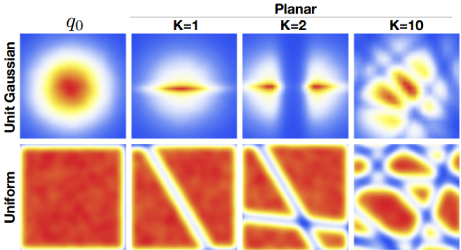
\includegraphics[scale=0.4]{pics/normflows.png} \\
\vspace{5mm}
(from \cite{Rezende2015})
\end{frame} 
%\subsubsection{IWAE}
\begin{frame}
\thetitle{Importance Weighted Autoencoder (IWAE)~\citep{Burda2015}}
\begin{itemize}
    \item Flows are a way of tightening the ELBO by making the variational family more flexible. 
    \item Not the only way: can obtain a tighter lower bound on $\log p(x \param \theta)$ by using multiple importance samples.
\end{itemize}

    \air
    \air

    Consider:
    \begin{align*}
        I_K = \frac{1}{K} \sum_{k=1}^K \frac{p(x, z^{(k)} \param \theta)}{q(z^{(k)} \given x \param \lambda)},
    \end{align*}
    where each $z^{(k)} \sim q(z \given x \param \lambda)$.
    
    \air
    \air
    Note that $I_K$ is an unbiased estimator of $p(x \param \theta)$:
    \begin{align*}
        \E_{q(z^{(1:K)} \given x \param \lambda)} \left[I_K \right] = p(x \param \theta).
    \end{align*}

\air
% 
\end{frame}

\subsection{IWAE}

\begin{frame}
\thetitle{Importance Weighted Autoencoder (IWAE)~\citep{Burda2015}}
    \textit{Any} unbiased estimator of $p(x \param \theta)$ can be used to obtain a lower bound, using Jensen's inequality:
    \begin{align*}
        p(x \param \theta) &= \E_{q(z^{(1:K)} \given x \param \lambda)} \left[ I_K \right] \\
        \implies \log p(x \param \theta) &\geq \E_{q(z^{(1:K)} \given x \param \lambda)} \left[ \log I_K \right] \\
        &= \E_{q(z^{(1:K)} \given x \param \lambda)} \left[ \log \frac{1}{K} \sum_{k=1}^K \frac{p(x, z^{(k)} \param \theta)}{q(z^{(k)} \given x \param \lambda)} \right]
    \end{align*}

However, can also show~\citep{Burda2015}:
\begin{itemize}
    \item $\log p(x \param \theta) \geq \E \left[ \log I_K \right] \geq \E \left[ \log I_{K-1} \right]$
    \item $\lim_{K \rightarrow \infty} \E \left[ \log I_K \right] = \log p(x \param \theta)$ under mild conditions
\end{itemize}
\end{frame}

\begin{frame}
\thetitle{Importance Weighted Autoencoder (IWAE)~\citep{Burda2015}}
\[ \E_{q(z^{(1:K)} \given x \param \lambda)} \left[ \log \frac{1}{K} \sum_{k=1}^K \frac{p(x, z^{(k)} \param \theta)}{q(z^{(k)} \given x \param \lambda)} \right] 
\]
    \begin{itemize}
      \item Note that with $K=1$, we recover the ELBO.
      \item Can interpret $\frac{p(x, z^{(k)} \param \theta)}{q(z^{(k)} \given x \param \lambda)}$ as importance weights.
        \item If $q(z \given x \param \lambda)$ is reparameterizable, we can use the reparameterization trick to optimize $\E \left[ \log I_K \right]$ directly.
        \item Otherwise, need score function gradient estimators \citep{Mnih2016}.
    \end{itemize}
\end{frame}




\section{Applications}

\subsection{Sentence VAE}
\begin{frame}
\thetitle{Sentence VAE Example \citep{Bowman2016}}
Generative Model (Model 2):
\begin{itemize}
    \item Draw $\boldz \sim \mathcal{N}(\mathbf{0}, \mathbf{I})$
    \item Draw $x_{t} \given  \boldz \sim \CRNNLM( \theta, \boldz)$
    %p(x_t \given x_{<t},\boldz \param \theta)$
    %\item Draw $x_{t+1} \given x_{<t}, \boldz \sim \softmax(\mathbf{W}\boldh_{\boldz,t})$ %p(x_t \given x_{<t},\boldz \param \theta)$
    % \[  \]
    % \[ p(x_t \given x_{<t}, \boldz ) = \softmax(\mathbf{W}\boldh_{\boldz,t-1})_{x_t}\]

\end{itemize}

Variational Model (Amortized): Deep Diagonal Gaussians, 
\[ q(\boldz \given x \param \lambda ) = \mathcal{N}(\boldsymbol{\mu}, \boldsymbol{\sigma^2}) \]
\[ \tilde{\boldh}_T = \RNN(x; \psi) \]
\[ \boldsymbol{\mu} = \mathbf{W}_1\tilde{\boldh}_T \,\,\,\,\,\,\,\,\,\, \boldsymbol{\sigma^2} = \exp(\mathbf{W}_2 \tilde{\boldh}_T)\ \ \ \lambda = \{\mathbf{W}_1, \mathbf{W}_2, \psi\}\]
\end{frame}


\begin{frame}
\thetitle{Sentence VAE Example \citep{Bowman2016}}
\center
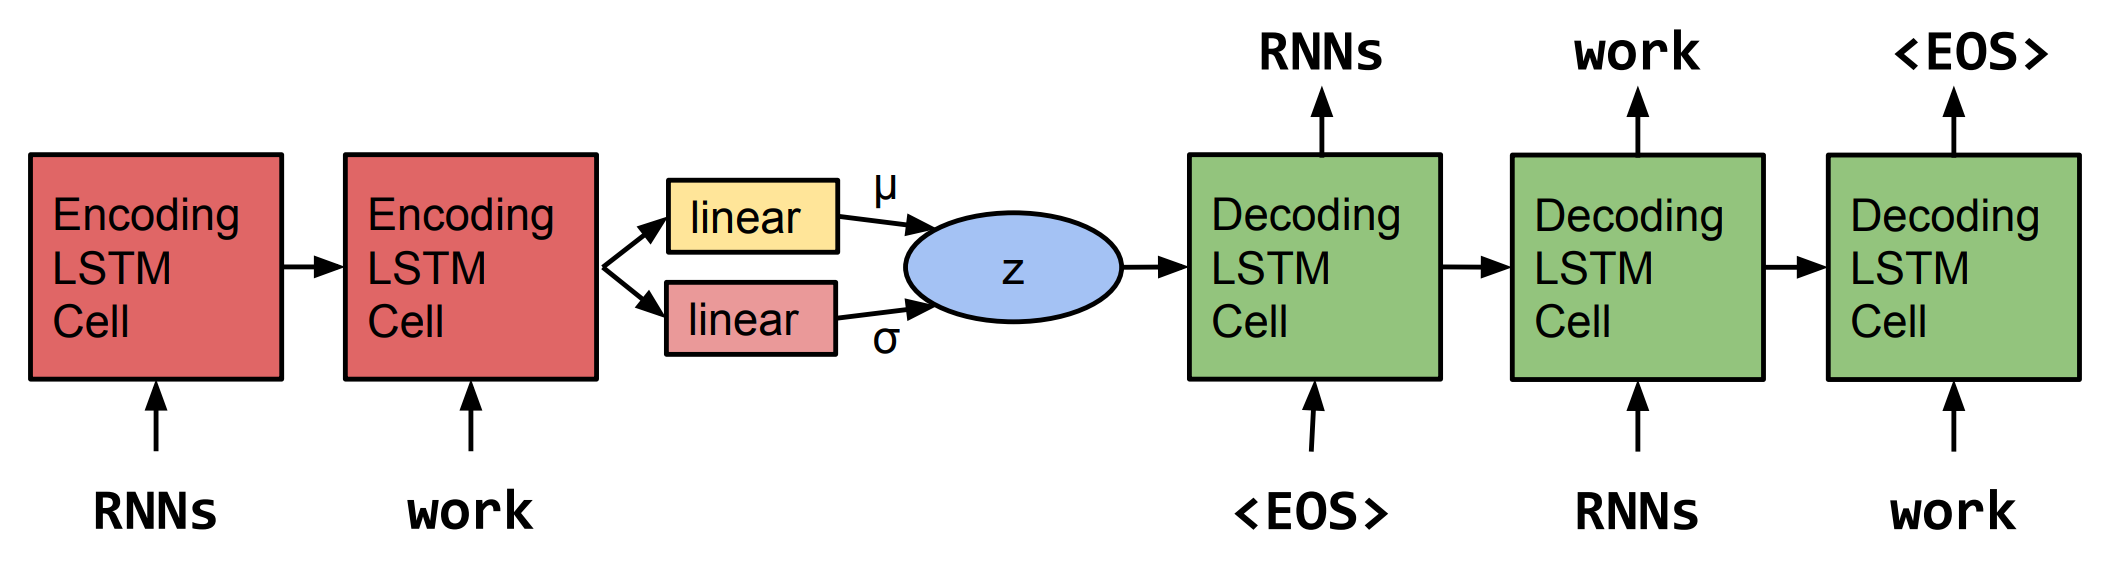
\includegraphics[scale=0.33]{pics/seq2seq_vae_text.png} \\

(from \cite{Bowman2016})

\begin{center}
\begin{tikzpicture}

     \node[latent] (zl) {$z$};%
     \node[const, below=of zl] (xl) {$x^{}$};%
     \node[const, left=of zl] (lambda) {$\lambda$};
     \edge{lambda}{zl};
     \edge{xl}{zl};
    
    \begin{scope}[xshift=5cm, yshift=-1cm]
% nodes
\node (dots) {$\ldots$};%
 \node[obs, left=1cm of dots] (x1) {$x_1^{}$};%
 \node[obs, right=1cm of dots] (xT) {$x_T^{}$};%
 \node[latent, above=5mm of dots] (z) {$z$}; %

 \edge {z} {dots};
 \edge {z} {x1};
 \edge {z} {xT};
 %\edge {mu} {z};
 %\edge {sigma} {z};
 \edge {x1} {dots};
 %\edge[bend left] {x1.south} {xT.south};
  \edge {dots} {xT};
% \edge {pi.east} {x1,xT.south};

 \draw[->] 
 (x1) edge[bend right] node [right] {} (xT);
 %\draw[->]
 %(dots) edge[bend right] node [right] {} (xT);

\end{scope}

 \node(eps)[latent,  above = 5mm of z]{$\epsilon$};
%  \draw[->, decorate, decoration={zigzag,
%     segment length=4,
%     amplitude=.9,post=lineto,
%     post length=2pt}] (eps) -- (z);
\draw (eps) edge[->] node (mid){} (z);
\draw (zl) edge[dashed]  (mid);

\end{tikzpicture}
\end{center}
\end{frame}

% \begin{frame}
% \thetitle{Text VAE Example \citep{Bowman2016}}

% Objective (for single data point):
% \begin{align*}
%     &\ELBO(\theta, \phi \param x) = \E_{q(\boldz \given x \param \phi)}\Big[\log \frac{p(x, \boldz \param \theta)}{q(\boldz \given x \param \phi)} \Big] \\
%     &= \E_{q(\boldz \given x \param \phi)}[\log p(x \given \boldz \param \theta) ] - \KL[q(\boldz \given x \param \phi) \Vert p(\boldz)]
% \end{align*}
% Gradient with regard to $\theta$: 
% \[ \nabla_\theta \ELBO(\theta, \phi \param x) = \E_{q(\boldz \given x \param \phi)}[\nabla_\theta \log p(x \given \boldz \param \theta) ]  \]
% (expectation approximated with a single sample)
% \end{frame}

% \begin{frame}
% \thetitle{Text VAE Example \citep{Bowman2016}}
% Gradient with regard to $\phi$:
% \\ First note 
% \[\KL[q(\boldz \given x \param \phi) \Vert p(\boldz)]  = -\frac{1}{2}\sum_{j=1}^d (\log \boldsymbol{\sigma}^2_j - \boldsymbol{\sigma}^2_j - \boldsymbol{\mu}_j^2 + 1) \]
% So $\nabla_\phi \KL[q(\boldz \given \boldx \param \phi) \Vert p(\boldz)]$ is easy. \\
% \[ \, \]
% Much harder:
% \[ \nabla_\phi \E_{q(\boldz \param x \param \phi)}[\log p( x \given \boldz \param \theta)]\]
% \end{frame}

% \begin{frame}
% \thetitle{Text VAE Example \citep{Bowman2016}}
% In the general case, use score function gradient estimator (aka REINFORCE \citep{Williams1992})
% \begin{align*}
%     & \nabla_\phi \E_{q(\boldz \given x \param \phi)}[\log p( x \given \boldz \param \theta)] = \nabla_\phi \int \log p(x \given \boldz \param \phi) q(\boldz \given x \param \phi)d\boldz \\
%     &= \int \log p(x \given \boldz \param \theta) \nabla_\phi q(\boldz \given x \param \phi)d\boldz \\
%      &= \int \log p(x \given \boldz \param \theta)  q(\boldz \given x \param \phi) \nabla_\phi \log  q(\boldz \given x \param \phi) d\boldz \\   
%           &=   \E_{q(\boldz \given x \param \phi)}[\log p(x \given \boldz \param \theta)  \nabla_\phi \log  q(\boldz \given x \param \phi)]
% \end{align*} 
% (since $\nabla p = p \nabla \log p$)\\

% And we can against estimate the gradient with samples from $q(\boldz \given x \param \phi)$
% \end{frame}


% \begin{frame}
% \thetitle{Text VAE Example \citep{Bowman2016}}
% The reparameterization trick: under our choice of $\mathcal{Q}$, we can draw a sample from $\boldq(\boldz \given \boldx \param \phi)$ by
% \[ \boldsymbol{\epsilon} \sim \mathcal{N}(\mathbf{0}, \mathbf{I}) \,\,\,\,\,\,\,\,\,\,\,\,\,\,\, \boldz =  \boldsymbol{\mu} + \boldsymbol{\epsilon}\boldsymbol{\sigma}\]
% Then
% \begin{align*}
%     \nabla_\phi \E_{q(\boldz \given x \param \phi)}[\log p( &x \given \boldz \param \theta)] \\  &= \nabla_\phi \E_{\epsilon \sim \mathcal{N}(\mathbf{0}, \mathbf{I})}[\log p( x \given  \boldsymbol{\mu} + \boldsymbol{\epsilon}\boldsymbol{\sigma} \param \theta)] \\
%     &= \E_{\epsilon \sim \mathcal{N}(\mathbf{0}, \mathbf{I})}[\nabla_\phi \log p(x \given  \boldsymbol{\mu} + \boldsymbol{\epsilon}\boldsymbol{\sigma} \param \theta)] 
%     \end{align*}
%     Empirically yields much lower-variance gradient estimators.
% \end{frame} 

% \begin{frame}
% \thetitle{Text VAE Example \citep{Bowman2016}}
% The reparameterization trick
% \center
% 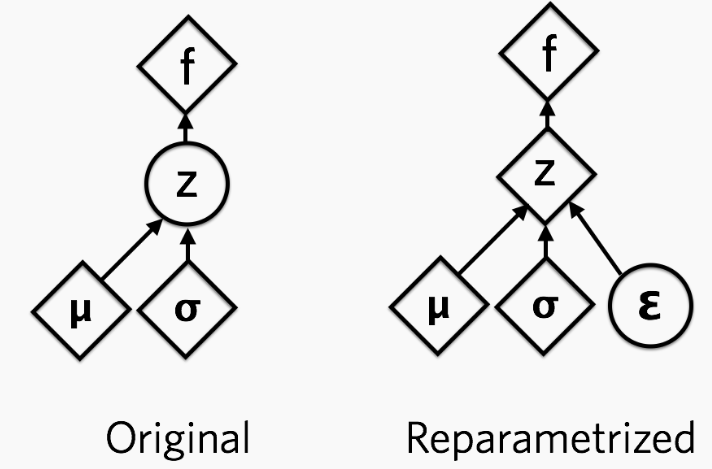
\includegraphics[scale=0.35]{pics/reparam.png}
% \end{frame} 

\begin{frame}
\thetitle{Issue 1: Posterior Collapse}

\vspace{-0.5cm}

\begin{eqnarray*} 
\ELBO(\theta, \lambda) &=  \E_{q(z \given x \param \lambda)}[\log \frac{p( x, z \param \theta)}{ q(z \given x \param \lambda)}] \\\\
&= \underbrace{\E_{q(z \given x \param \lambda)}[\log p( x \given z \param \theta)]
}_{\text{Reconstruction likelihood}} - \underbrace{\KL[q(z \given x \param \lambda) \Vert p(z)]}_{\text{Regularizer}} 
\end{eqnarray*}
\center
\vspace{5mm}

\begin{tabular}{l c c c }
\toprule
     Model & L/ELBO & Reconstruction & KL \\
\midrule     
     RNN LM & -329.10 & - & - \\
     RNN VAE & -330.20 & -330.19 & 0.01 \\
\bottomrule
\end{tabular} \\
\vspace{5mm}
(On Yahoo Corpus from \cite{Yang2017}) \\
\end{frame} 

\begin{frame}
\thetitle{Issue 1: Posterior Collapse}
\begin{itemize}
%   \item Posterior collapse: $x$ and $z$ are independent and the generative model $p(x, z \param \theta)$
%     reduces to a standard language model (without latent variables).

  \item $x$ and $z$ become independent, and $p(x, z \param \theta)$
    reduces to a non-LV language model.    
    
    \air
    % \item \citet{Chen2017}: With a fully autoregressive/powerful likelihood model $p(x \given z \param \theta)$,    if it is possible to model $p_\star(x)$ without making use of $z$, then optimum is at
    \item \citet{Chen2017}: If it's possible to model $p_\star(x)$ without making use of $z$, then ELBO optimum is at:    
    \[ p_\star(x) = p(x \given z \param \theta) = p(x \param \theta) \ \ \ \ q(z \given x \param \lambda) = p(z) \]
    \[ \KL[q(z \given x \param \lambda) \Vert p(z)] = 0\] 
\end{itemize}
\end{frame} 

\begin{frame}
\thetitle{Mitigating Posterior Collapse}
Use less powerful likelihood models~\citep{Miao2016,Yang2017},
or ``word dropout" \citep{Bowman2016}. \\
\vspace{2mm}
\center
\begin{tabular}{l c c c }
\toprule
     Model & LL/ELBO & Reconstruction & KL \\
\midrule     
     RNN LM & -329.1 & - & - \\
     RNN VAE & -330.2 & -330.2 & 0.01 \\
     $\,\,\,\,$ + Word Drop & -334.2 & -332.8 & 1.44\\
     CNN VAE & -332.1 & -322.1 & 10.0 \\ 
\bottomrule
\end{tabular} \\
\vspace{5mm}
(On Yahoo Corpus from \cite{Yang2017}) \\
\end{frame} 

\begin{frame}
\thetitle{Mitigating Posterior Collapse}
Gradually anneal multiplier on KL term, i.e.
\[\E_{q(z \given x \param \lambda)}[\log p( x \given z \param \theta)] - \beta\KL[q(z \given x \param \lambda) \Vert p(z)] \]
$\beta$ goes from 0 to 1 as training progresses
\\
\center
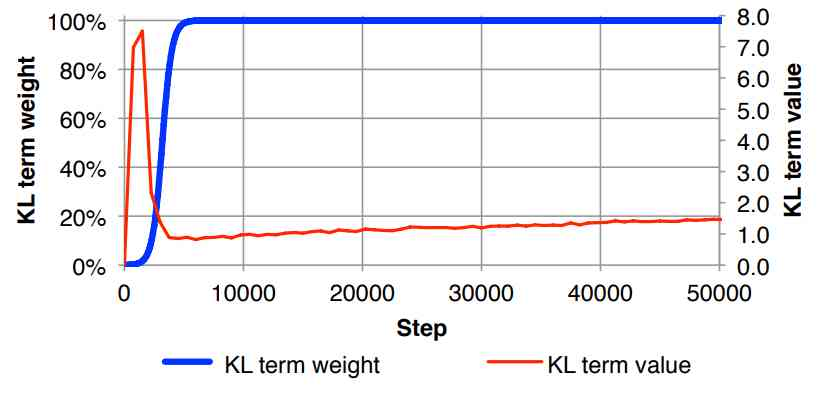
\includegraphics[scale=0.25]{kllambda.jpg}
\\
(from \cite{Bowman2016})
\end{frame} 

\begin{frame}
\thetitle{Mitigating Posterior Collapse}
Other approaches:
\begin{itemize}
    \item Use auxiliary losses (e.g. train $z$ as part of a topic model) \citep{Dieng2017,wang2017topic}
    \item Use von Mises--Fisher distribution with a fixed concentration parameter  \citep{Guu2017,xu2018}
    \item Combine stochastic/amortized variational inference \citep{Kim2018}
    \item Add skip connections \citep{dieng2018}
\end{itemize}
\air
\air
In practice, often necessary to combine various methods.
\end{frame} 

\begin{frame}
\thetitle{Issue 2: Evaluation}
\begin{itemize}
    \item ELBO always lower bounds $\log p(x \param \theta)$, so can calculate an upper bound on PPL efficiently.
    \item When reporting ELBO, should also separately report,
    \[ \KL[q(z \given x \param \lambda) \Vert p(z)] \] 
    to give an indication of how much the latent variable is being ``used".
\end{itemize}
\end{frame} 

\begin{frame}
\thetitle{Issue 2: Evaluation}
    
    Also can evaluate $\log p(x \param \theta)$ with importance sampling
    \begin{align*}
        p(x \param \theta) &= \E_{q(z \given x \param \lambda)}\Big[\frac{p(x \given z \param \theta)p(z)}{q(z \given x \param \lambda)}\Big] \\
        &\approx \frac{1}{K}\sum_{k=1}^K \frac{p(x | z^{(k)} \param \theta)p(z^{(k)})}{q(z^{(k)} \given x \param \lambda)}
    \end{align*}
    So 
    \[ 
    \implies \log p(x \param \theta) \approx \log \frac{1}{K}\sum_{k=1}^K \frac{p(x | z^{(k)} \param \theta)p(z^{(k)})}{q(z^{(k)} \given x \param \lambda)}
\]
%(biased but consistent estimator)
\end{frame} 

\begin{frame}
\thetitle{Evaluation}
Qualitative evaluation 
\begin{itemize}
    \item Evaluate samples from prior/variational posterior. 
    \item Interpolation in latent space. 
\center
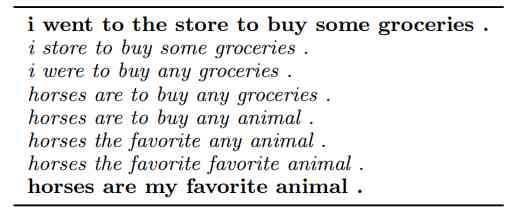
\includegraphics[scale=0.5]{pics/zinterp.jpg} \\
(from \cite{Bowman2016})
\end{itemize}
\end{frame} 

\subsection{Encoder/Decoder with Latent Variables}

\newcommand{\benc}{\boldsymbol{\mathrm{enc}}}

\begin{frame}
\thetitle{Encoder/Decoder ~\citep{Sutskever2014,Cho2014b}}
\begin{center}
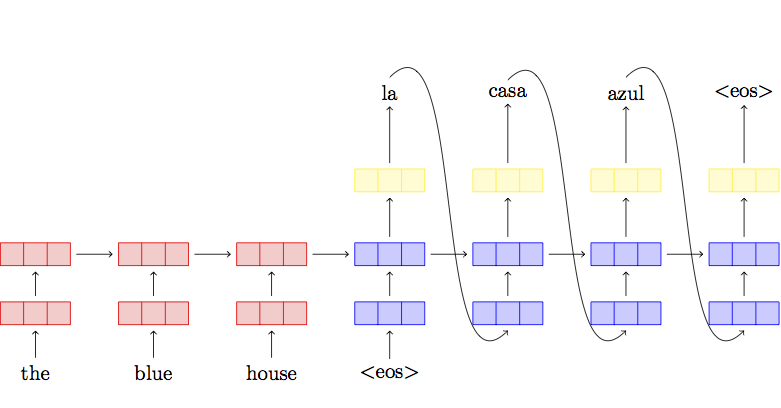
\includegraphics[scale=0.55]{pics/seq2seq.png}
\end{center}

\textbf{Given:} Source information $s = s_1, \ldots, s_M$.
\air

\textbf{Generative process:}
  \begin{itemize}
     %\item Set $\boldh_t = \RNN(\boldh_{t-1}, [\boldx_t, \benc(s)])$.
      \item Draw $x_{1:T} \given s \sim \CRNNLM(\theta, \benc(s))$.
  \end{itemize}




\air
%Log likelihood: 
%$ \implies  p(x_{1:T} \given s \param \theta) =  \prod_{t=1}^T \RNN([ \boldh_{t-1}, \benc(s)])_{x_t}$.
    % \begin{align*}
    %     \log p(x_{1:T} \given s \param \theta) = \log \prod_{t=1}^T \softmax(\boldW \boldh_{t-1})_{x_t}.
    % \end{align*}
    % \begin{align*}
    %     p(x_1, \ldots, x_T \given s \param \theta) &= \prod_{t=1}^T p(x_t \given x_{<t}, s \param \theta) \\
    %     &= \prod_{t=1}^T \softmax(\boldW \boldh_{t-1})_{x_t},
    % \end{align*}
\end{frame}

\begin{frame}
\thetitle{Latent, Per-token Experts~\citep{yang2018breaking}}

\textbf{Generative process:} For $t=1, \ldots, T$,
\begin{itemize}
    %\item Set $\boldh_t = \RNN([\boldx_t, \benc(s)], \boldh_{t-1})$.
    \item Draw $z_{t} \given x_{< t}, s \sim \softmax(\boldU \boldh_{t-1})$.
    \item Draw $x_{t} \given z_{t}, x_{< t}, s \sim \softmax(\boldW \tanh(\boldQ_{z_t} \boldh_{t-1}) \param \theta)$ %\text{Cat}(\softmax(\boldW \tanh(\boldQ_{z_t} \boldh_t)))$.
\end{itemize}
\begin{center}

\begin{tikzpicture}
  %\tikz{
% nodes
\node (dots) {$\ldots$};%
 \node[obs, left=1cm of dots] (x2) {$x_2^{(n)}$};%
 \node[obs, left=1cm of x2] (x1) {$x_1^{(n)}$};%
 \node[obs, right=1cm of dots] (xT) {$x_T^{(n)}$};%
 \node[latent, above=of x1] (z1) {$z_1^{(n)}$}; %
 \node[latent, above=of x2] (z2) {$z_2^{(n)}$}; %
 \node[latent, above=of xT] (zT) {$z_T^{(n)}$}; %
 %\node[const, above=(0.5cm) of z] (mu) {$\mu$};
 %\node[const, below left=0.3cm and 0.8cm of x1] (pi) {$\pi$};
 
% plate
 \plate {plate1} {(dots)(x1)(x2)(xT)(z1)(z2)} {$N$}; %
% edges

 \edge {x1} {zT};
 \edge {x2} {zT};
 \edge {dots} {zT};
 
 \edge {x1} {z2};

 \edge {z1} {x1};
 \edge {z2} {x2};
 \edge {zT} {xT};
 %\edge {mu} {z};
 %\edge {pi.east} {x1,xT.south};
 \edge {x1} {x2};
 \edge {x2} {dots};
 %\edge[bend left] {x1.south} {xT.south};
  \edge {dots} {xT};

 \draw[->] 
 (x1) edge[bend right=20] node [right] {} (xT);
 %}
 \end{tikzpicture}
 %}
\end{center}
\air 
\air
If $\boldU \in \reals^{K \times d}$, used $K$ experts; increases the flexibility of per-token distribution.

\end{frame}

\begin{frame}
\thetitle{Case-Study: Latent Per-token Experts~\citep{yang2018breaking}}
\textbf{Learning:} $z_t$ are independent given $x_{<t}$, so we can marginalize at each time-step (Method 3: Conjugacy).
    \begin{align*}
        &\argmax_{\theta} \log p(x \given s \param \theta) =  \\
        &\argmax_{\theta} \log \prod_{t=1}^T \sum_{k=1}^K p(z_t {=} k \given s, x_{<t} \param \theta) \, p(x_t \given z_t{=}k, x_{<t}, s \param \theta).
    \end{align*}

\textbf{Test-time:}
\begin{align*}
\argmax_{x_{1:T}} \prod_{t=1}^T \sum_{k=1}^K p(z_t {=} k \given s, x_{<t} \param \theta) \, p(x_t \given z_t{=}k, x_{<t}, s \param \theta).
\end{align*}
\end{frame}

\begin{frame}
    \thetitle{Case-Study: Latent, Per-token Experts~\citep{yang2018breaking}}
PTB language modeling results ($s$ is constant):
\air
\begin{table}
\begin{tabular}{lc}
\toprule
     Model & PPL \\
\midrule     
     \citet{merity2018regularizing} & 57.30 \\
     Softmax-mixture~\citep{yang2018breaking} & 54.44 \\
\bottomrule
\end{tabular}  
\end{table}

\air
\air
        
Dialogue generation results ($s$ is context):
\air
\begin{table}
\begin{tabular}{lcc}
\toprule
     Model &  \multicolumn{2}{c}{BLEU} \\
     & Prec & Rec \\
\midrule     
     No mixture & 14.1 & 11.1 \\
     Softmax-mixture~\citep{yang2018breaking} & 15.7 & 12.3 \\
\bottomrule
\end{tabular}
\end{table}
    
\end{frame}

\begin{frame}
\thetitle{Attention~\citep{Bahdanau2015}}
\begin{center}
    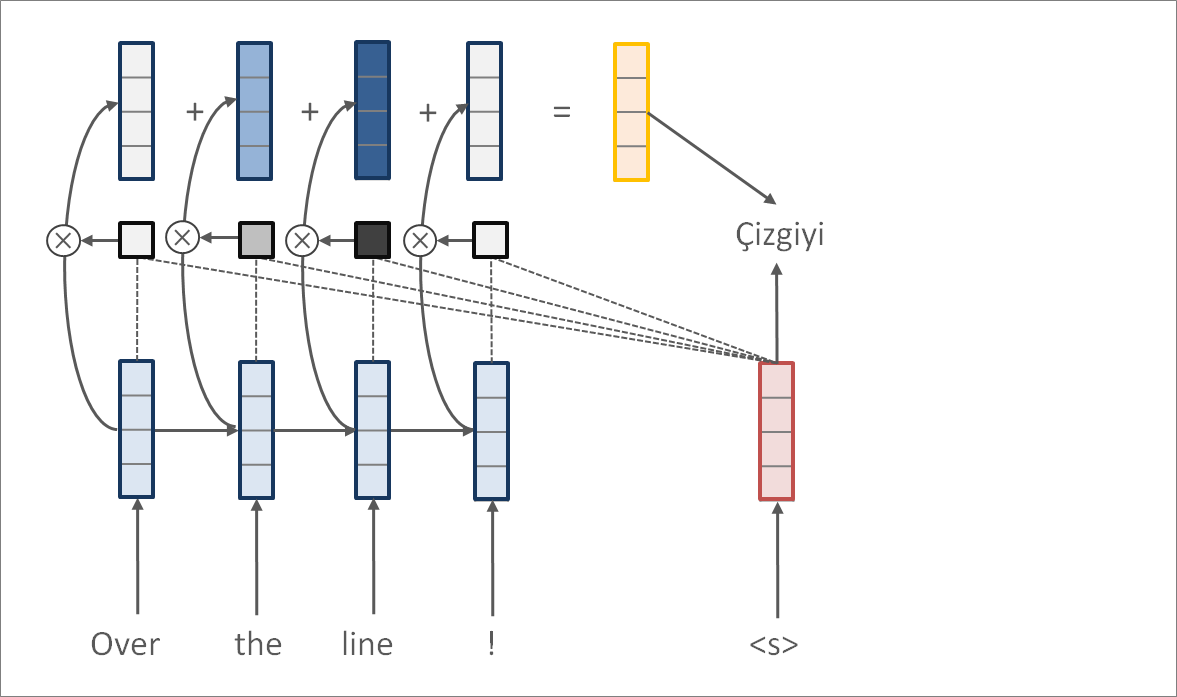
\includegraphics[scale=0.24]{pics/attn1step.png}
\end{center}

Decoding with an attention mechanism:

\[x_{t} \given x_{< t}, s  \sim \softmax(\boldW [\boldh_{t}, {\sum_{m=1}^M} \alpha_{t,m} \,  \benc(s)_m]).\]


% \air
% \begin{itemize}
%     \item Learning the same as in standard encoder/decoder.
% \end{itemize}

\end{frame}

\begin{frame}
\thetitle{Copy Attention \citep{gu2016incorporating,gulcehre2016pointing}}
Copy attention models copying words directly from $s$.
\air


\textbf{Generative process:} For $t=1, \ldots, T$,
\begin{itemize}
    %\item Set $\boldh_t = \RNN([\boldx_t, \benc(s)], \boldh_{t-1})$.
    \item Set $\balpha_t$ to be attention weights.
    \item Draw $z_{t} \given x_{< t}, s \sim \mathrm{Bern}(\MLP([\boldh_{t}, \benc(s)]))$.
    \item If $z_{t} = 0$
    \begin{itemize}
        \item Draw $x_{t} \given z_{t}, x_{< t}, s \sim \softmax(\boldW \boldh_{t})$.
    \end{itemize}
    \item Else 
    \begin{itemize}
        \item Draw $x_{t} \in \{s_1, \ldots, s_M\} \given z_{t}, x_{< t}, s \sim \mathrm{Cat}(\balpha_t)$.

    \end{itemize}
    \end{itemize}

\end{frame}

\begin{frame}
\thetitle{Copy Attention}
\textbf{Learning:} Can maximize the log per-token marginal~\citep{gu2016incorporating}, as with per-token experts:
        \begin{align*}
        &\max_{\theta} \log p(x_1, \ldots, x_T \given s \param \theta) \\
        = &\max_{\theta} \log \prod_{t=1}^T \sum_{z' \in\{0, 1\}} p(z_t = z' \given s, x_{<t} \param \theta) \, p(x_t \given z', x_{<t}, x \param \theta).
    \end{align*}
    
    \air
    \air
\textbf{Test-time:}
\begin{align*}
\argmax_{x_{1:T}} \prod_{t=1}^T \sum_{z' \in\{0, 1\}} p(z_t {=} z' \given s, x_{<t} \param \theta) \, p(x_t \given z', x_{<t}, s \param \theta).
\end{align*}
\end{frame}

\begin{frame}
\thetitle{Attention as a Latent Variable~\citep{deng2018}}


\textbf{Generative process:} For $t=1, \ldots, T$,
\begin{itemize}
    %\item Set $\boldh_t = \RNN([\boldx_t, \benc(s)], \boldh_{t-1})$.
    \item Set $\balpha_t$ to be attention weights.
    \item Draw $z_{t} \given x_{ < t}, s \sim \mathrm{Cat}(\balpha_t)$.
    \item Draw $x_{t} \given z_{t}, x_{< t}, s \sim \softmax(\boldW [\boldh_{t-1}, \benc(s_{z_{t}})] \param \theta)$.
\end{itemize}

% \air
% \air
% Note $\bolda_t \in \Delta^{M-1}$.
\end{frame}

\begin{frame}
\thetitle{Attention as a Latent Variable~\citep{deng2018}}
Marginal likelihood under latent attention model:
    \begin{align*}
       p(x_{1:T} \given s \param \theta) = \prod_{t=1}^T \sum_{m=1}^M \alpha_{t,m} \softmax(\boldW [\boldh_{t-1}, \benc(s_{m})] \param \theta)_{x_t}.
    \end{align*}
    
\air
\air
\air
\air

Standard attention likelihood:
    \begin{align*}
        p(x_{1:T} \given s \param \theta) = \prod_{t=1}^T  \softmax(\boldW [\boldh_{t-1}, \sum_{m=1}^M \alpha_{t,m} \, \benc(s_{m})] \param \theta)_{x_t}.
    \end{align*}
    % \begin{align*}
    %     p(x_{1:T} \given s \param \theta) = \prod_{t=1}^T  \RNN([\boldh_{t-1}, \sum_{m=1}^M \alpha_{t,m} \, \benc(s_{m})] \param \theta)_{x_t}.
    % \end{align*}
    
% \air
% \air
% Only the former corresponds to the marginal likelihood of a latent variable model.
\end{frame}

\begin{frame}
\thetitle{Attention as a Latent Variable~\citep{deng2018}}
\textbf{Learning Strategy \#1:} Maximize the log marginal via enumeration as above.

\air

\textbf{Learning Strategy \#2:} Maximize the ELBO with AVI:

\begin{align*}
    \max_{\lambda, \theta} \E_{q(z_t \param \lambda)} \left[ \log p(x_t \given x_{<t}, z_t, s) \right] - \KL[q(z_t \param \lambda) \Vert p(z_t \given x_{<t}, s)].
\end{align*}

\air

\begin{itemize}
    \item $q(z_t \given x \param \lambda)$ approximates $p(z_t \given x_{1:T}, s \param \theta)$; implemented with a BLSTM.
    \item $q$ isn't reparameterizable, so gradients obtained using REINFORCE + baseline.
\end{itemize}

\end{frame}


\begin{frame}
\thetitle{Attention as a Latent Variable~\citep{deng2018}}
\textbf{Test-time:} Calculate $p(x_t \given x_{<t}, s \param \theta)$ by summing out $z_t$.

\air
\air
MT Results on IWSLT-2014:
\begin{table}
\begin{tabular}{lcc}
\toprule
     Model & PPL & BLEU\\
\midrule     
     Standard Attn & 7.03 & 32.31 \\
     Latent Attn (marginal) & 6.33 & 33.08 \\ 
     Latent Attn (ELBO) & 6.13 & 33.09 \\
\bottomrule
\end{tabular}
\end{table}
\end{frame}

\begin{frame}
\thetitle{Encoder/Decoder with Structured Latent Variables}
At least two EMNLP 2018 papers augment encoder/decoder text generation models with \textit{structured} latent variables:

\begin{enumerate}
    \item \citet{lee2018deterministic} generate $x_{1:T}$ by iteratively refining sequences of words $z_{1:T}$.
    \air
    \air 
    \item \citet{wiseman2018learning} generate $x_{1:T}$ conditioned on a latent template or plan $z_{1:S}$.
\end{enumerate}
    
\end{frame}

\subsection{Latent Summaries and Topics}

\begin{frame}
\thetitle{Summary as a Latent Variable~\citep{miao2016language}}
Generative process for a document $x = x_1, \ldots, x_T$:
\begin{itemize}
    \item Draw a latent summary $z_1, \ldots, z_{M} \sim \RNNLM(\theta) $%p(z_1, \ldots, z_{M} \param \theta)$
    \item Draw $x_1, \ldots, x_{T} \given z_{1:M} \sim \CRNNLM(\theta, z) $ %p(x_1, \ldots, x_T \given z_{1:M} \param \theta)$
    %\item ($p(z \param \theta)$ and $p(x \given z \param \theta)$ modeled with encoder/decoder RNNs).
\end{itemize}

% \air
% \air
% \citet{miao2016language} parameterize prior $p(z)$ with an RNN, and generative model $p(x \given z)$ with encoder/decoder RNNs.
    
\air
\air
\air
\pause
%\textbf{Note:} previously we cared most about the model generating $x_{1:T}$; here we care most about \textit{inference}: 
Posterior Inference:
\begin{align*}
p(z_{1:M} \given x_{1:T} \param \theta) = p(\text{summary} \given \text{document} \param \theta).    
\end{align*}
\end{frame}

\begin{frame}
\thetitle{Summary as a Latent Variable~\citep{miao2016language}}
\textbf{Learning:} Maximize the ELBO with amortized  family:
\begin{align*}
    \max_{\lambda, \theta} \E_{q(z_{1:M} \param \lambda)} &\left[\log p(x_{1:T} \given z_{1:M} \param \theta) \right] - \KL[q(z_{1:M} \param \lambda) \Vert p(z_{1:M} \param \theta)]
\end{align*}

\begin{itemize}
    \item $q(z_{1:M} \param \lambda)$ approximates $p(z_{1:M} \given x_{1:T} \param \theta)$; also implemented with encoder/decoder RNNs.
    \item $q(z_{1:M} \param \lambda)$ not reparameterizable, so gradients use REINFORCE + baselines.
\end{itemize}

\end{frame}

\begin{frame}
\thetitle{Summary as a Latent Variable~\citep{miao2016language}}
\textbf{Semi-supervised Training:} Can also use documents \textit{without} corresponding summaries in training.
\begin{itemize}
    \item Train $q(z_{1:M} \param \lambda) \approx p(z_{1:M} \given x_{1:T} \param \theta)$ with labeled examples.
    \air
    \item Infer summary $z$ for an \textit{unlabeled} document with $q$.
    \air
    \item Use inferred $z$ to improve model $p(x_{1:T} \given z_{1:M} \param \theta)$.
    \air
    \item Allows for outperforming strictly supervised models!
\end{itemize}
\end{frame}


\begin{frame}
\thetitle{Topic Models~\citep{blei2003latent}}

\begin{center}
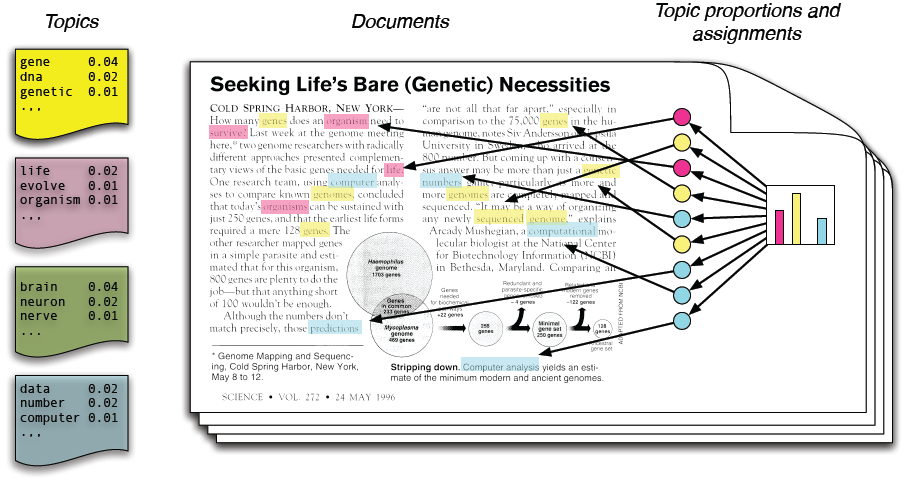
\includegraphics[scale=0.27]{pics/IntroToLDA.png}
\end{center}

Generative process: for each document $x^{(n)} = x^{(n)}_1, \ldots, x^{(n)}_T$,

\vspace{-2mm}
\begin{itemize}
    \item  Draw topic distribution $\boldz^{(n)}_{top} \sim Dir(\balpha)$
    \item  For $t=1, \ldots, T$:
    \begin{itemize}
        \item Draw topic $z^{(n)}_t \sim Cat(\boldz^{(n)}_{top})$
        \item Draw $x_t \sim Cat(\bbeta_{z^{(n)}_t})$
    \end{itemize}
\end{itemize}
    
\end{frame}

\begin{frame}
\thetitle{Simple, Deep Topic Models~\citep{miao2017nvi}}
\textbf{Motivation:} easy to learn deep topic models with VI if $q(\boldz^{(n)}_{top} \param \lambda)$ is reparameterizable.

\air
\air
\air
\textbf{Idea:} draw $\boldz^{(n)}_{top}$ from a transformation of a Gaussian.
\begin{itemize}
    \item Draw $\boldz^{(n)}_0 \sim \mcN(\bmu_0, \bsigma^2_0)$
    \item Set $\boldz^{(n)}_{top} = \softmax(\boldW \boldz^{(n)}_0)$. %, or to an even more complicated function of $\boldz^{(n)}_0$.
    \item Use analogous transformation when drawing from $q(\boldz^{(n)}_{top} \param \lambda)$.
    
\end{itemize}
    
\end{frame}


\begin{frame}
\thetitle{Simple, Deep Topic Models~\citep{miao2017nvi}}
\textbf{Learning Step \#1:} Marginalize out per-word latents $z^{(n)}_t$. 

\begin{align*}
    p(\{x^{(n)}\}_{n=1}^N, \{\boldz^{(n)}_{top}\}_{n=1}^N \param \theta) = \prod_{n=1}^N p(\boldz^{(n)}_{top} \given \theta) \prod_{t=1}^T \sum_{k=1}^K z^{(n)}_{top, k} \, \beta_{k, x^{(n)}_t}
\end{align*}

\air
\air
\textbf{Learning Step \#2:} Use AVI to optimize resulting ELBO.
\begin{align*}
    \max_{\lambda, \theta} \E_{q(\boldz^{(n)}_{top} \param \lambda)} &\left[\log p(x^{(n)} \given \boldz^{(n)}_{top}  \param \theta) \right] \\
    &- \KL[ \mcN(\boldz^{(n)}_0 \param \lambda) \Vert \mcN(\boldz^{(n)}_0 \param \bmu_0, \bsigma_0^2)]
\end{align*}
\end{frame}


\begin{frame}
\thetitle{Simple, Deep Topic Models~\citep{miao2017nvi}}
Perplexities on held-out documents, for three datasets:

\begin{table}
\begin{tabular}{lccc}
\toprule
     Model & MXM & 20News & RCV1 \\
\midrule     
     OnlineLDA~\citep{hoffman2010online} & 342 & 1015 & 1058 \\
     AVI-LDA~\citep{miao2017nvi} & 272 & 830 & 602 \\
\bottomrule
\end{tabular}
\end{table}




\end{frame}



\footnotesize
\bibliography{master}
\bibliographystyle{acl_natbib_nourl}
\end{document}
